\chapter{Additional materials for the bias study}
\label{sec:Appendix_bias}

\section{Linearity}
It was suggested to do the bias study with more signal events introduced when generating the pseudo-event. 
Following plots show how the mean and width of the pull distribution evolve as more signal events are introduced.
\clearpage
\subsection{$H\to \JPsi\ \gamma$}
\begin{figure}[!ht]
  \centering
  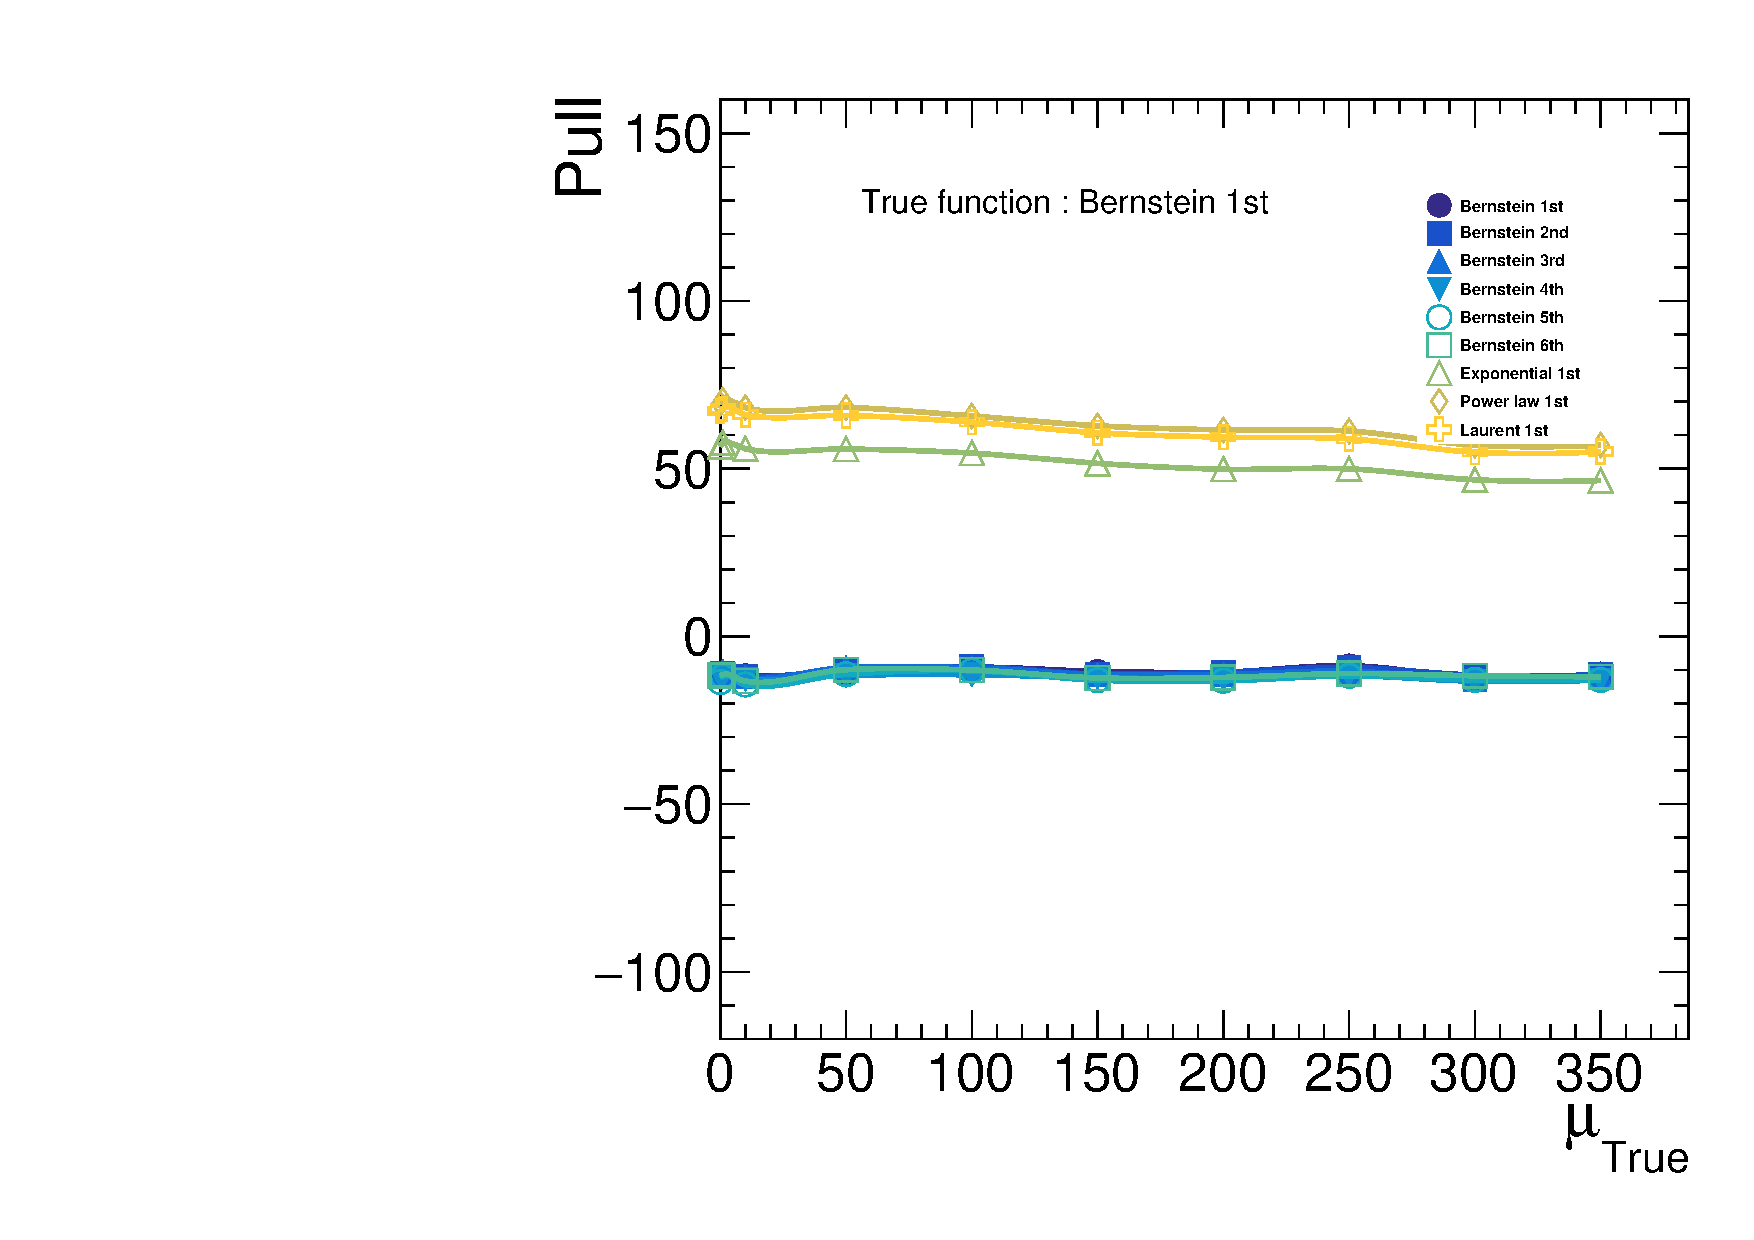
\includegraphics[width=0.33\textwidth]{Fig/BiasStudy/Linearity/HJpsiG/pull_mean_linearity_TrueFunc0}~
  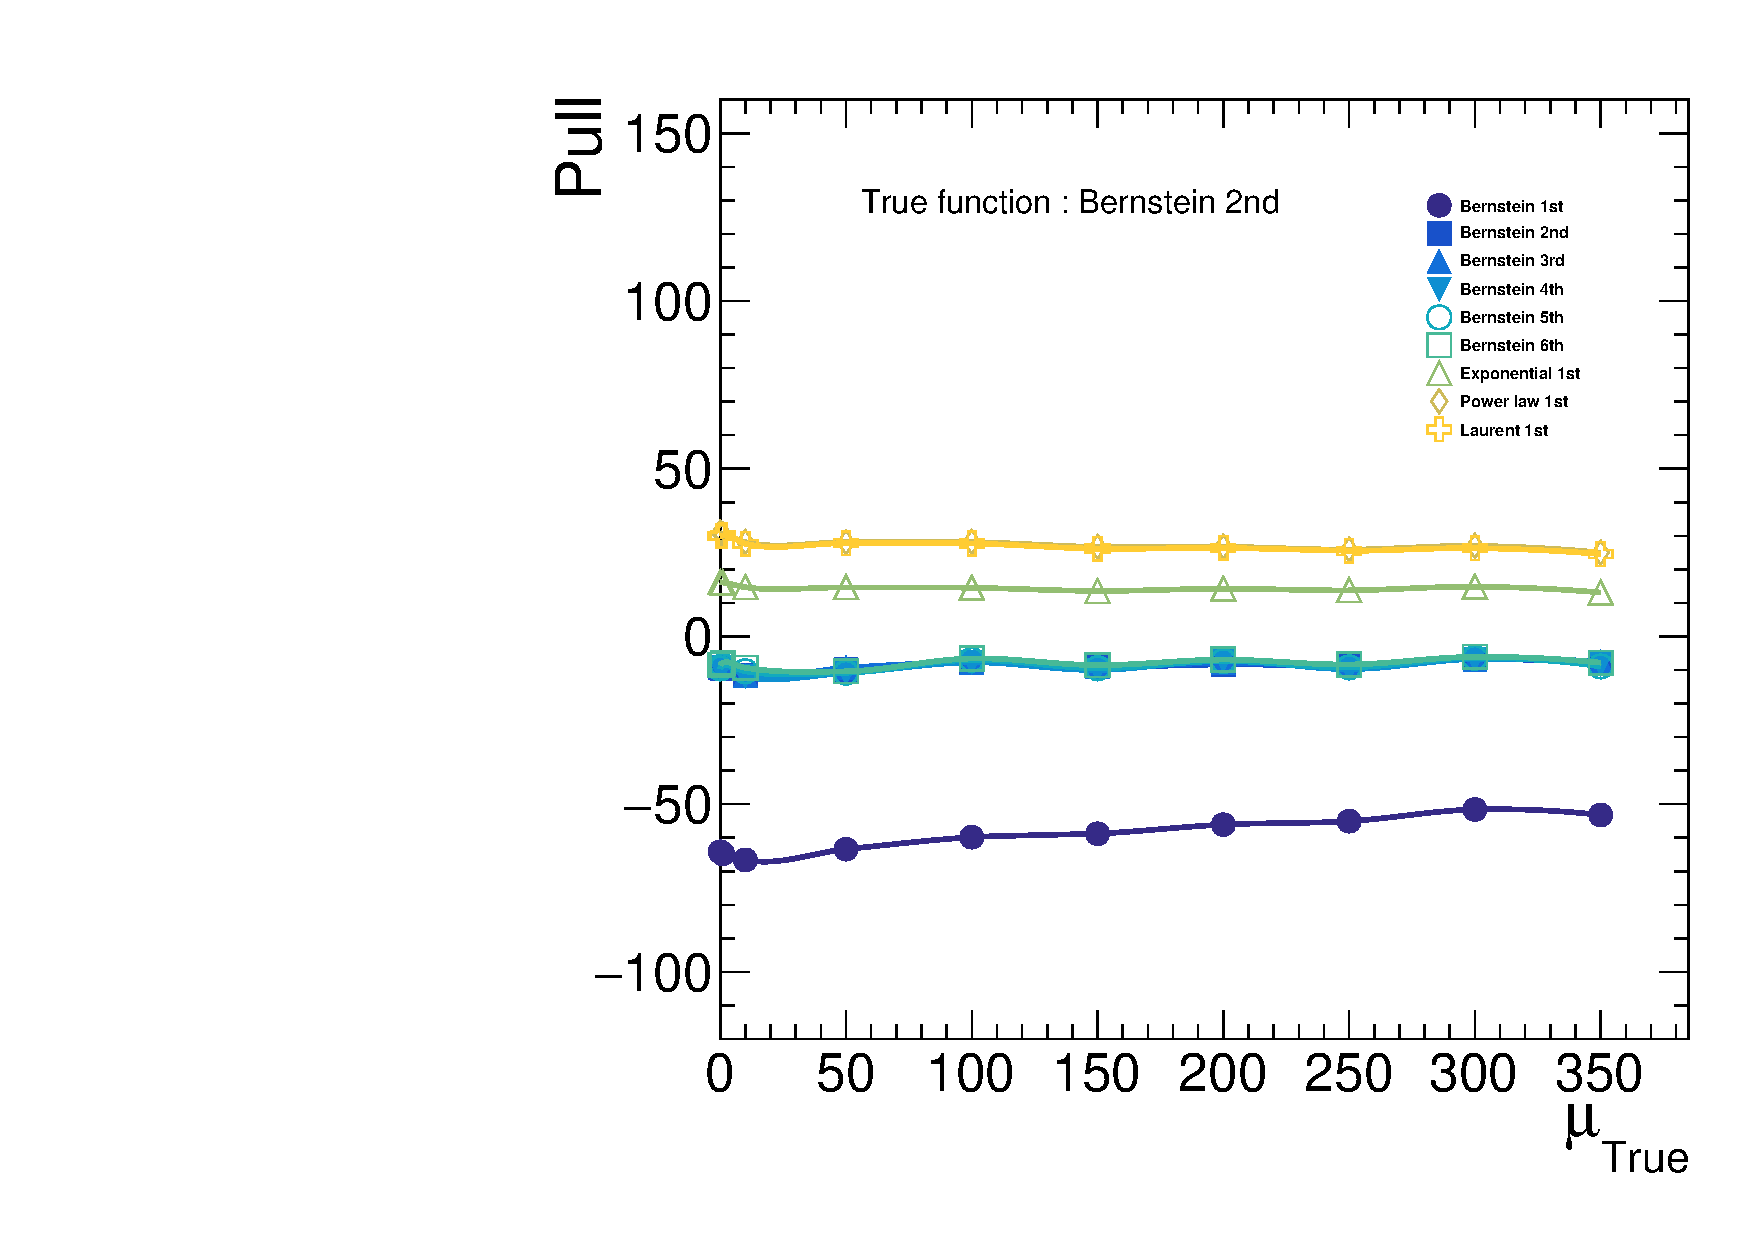
\includegraphics[width=0.33\textwidth]{Fig/BiasStudy/Linearity/HJpsiG/pull_mean_linearity_TrueFunc1}~
  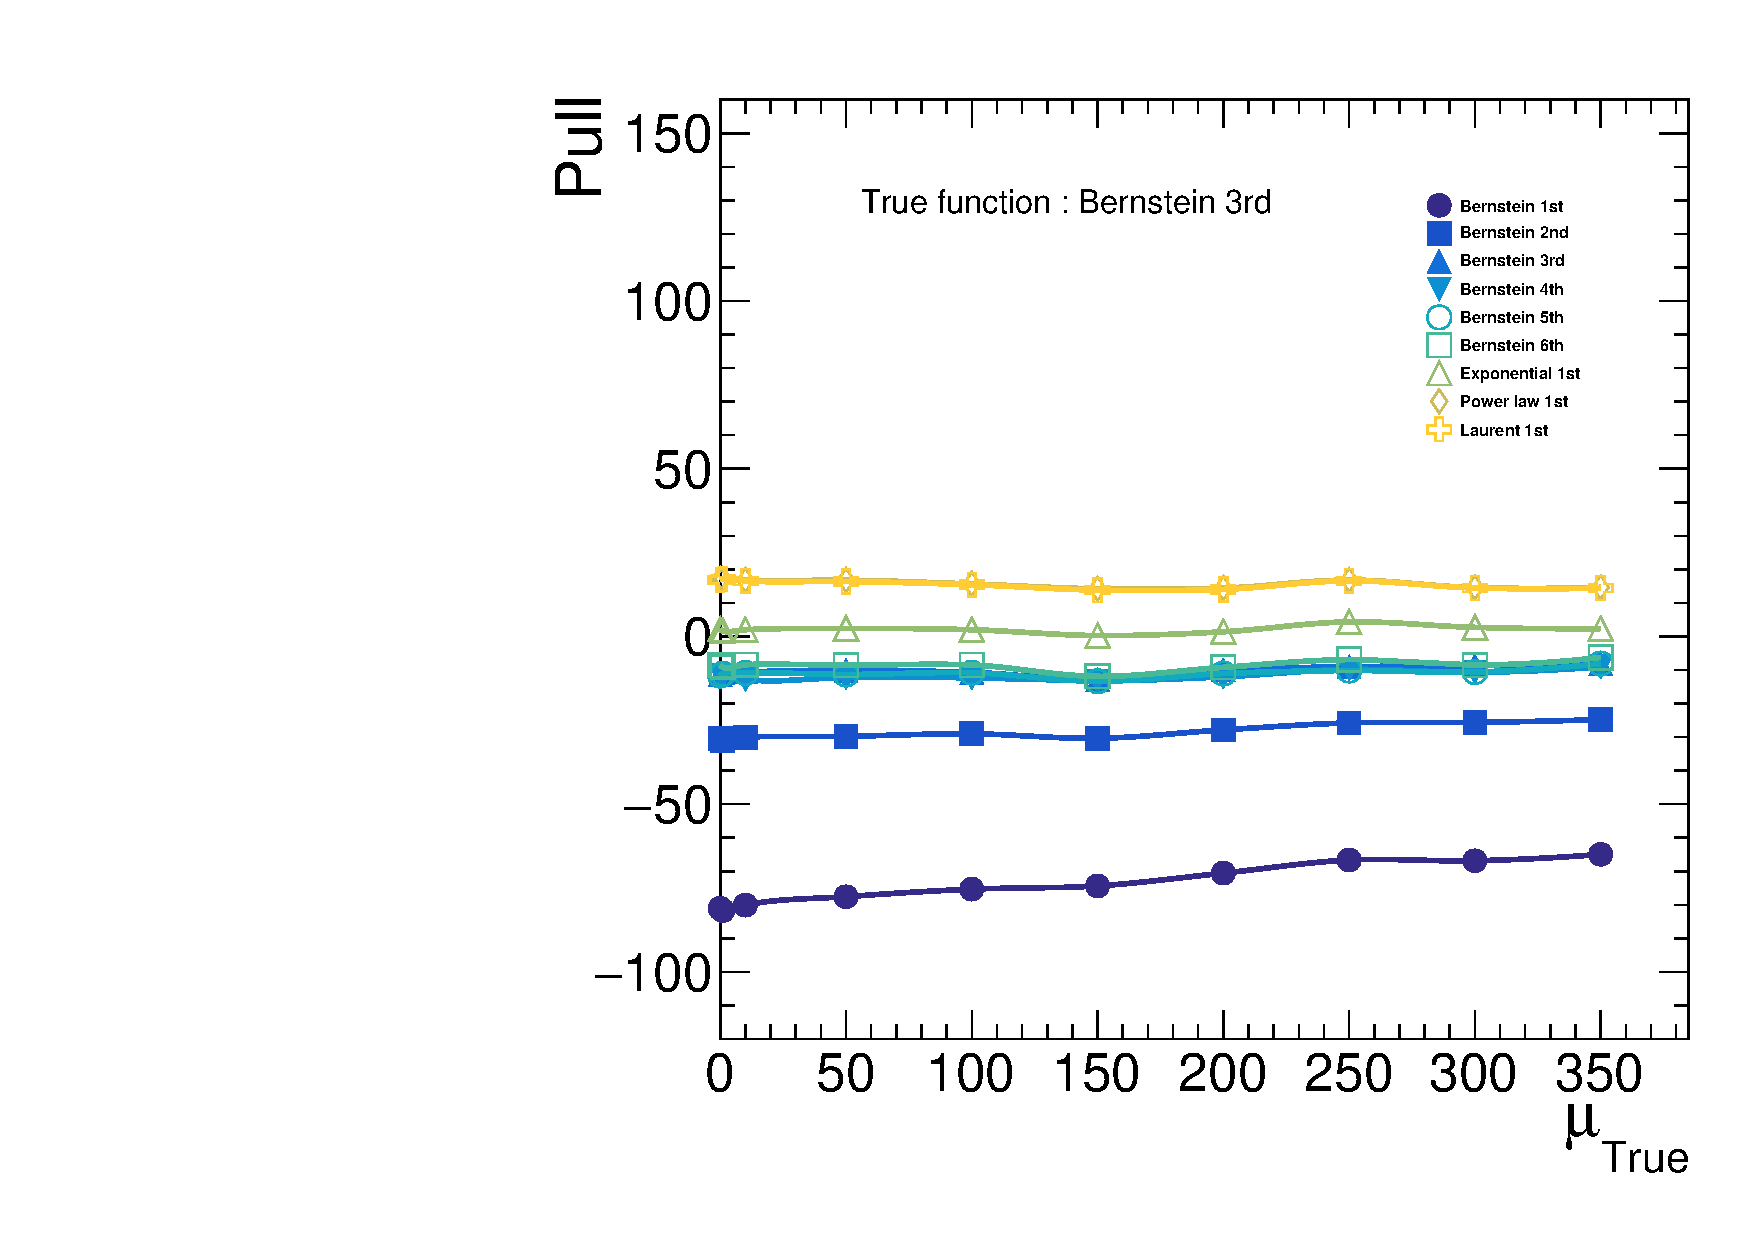
\includegraphics[width=0.33\textwidth]{Fig/BiasStudy/Linearity/HJpsiG/pull_mean_linearity_TrueFunc2}\\
  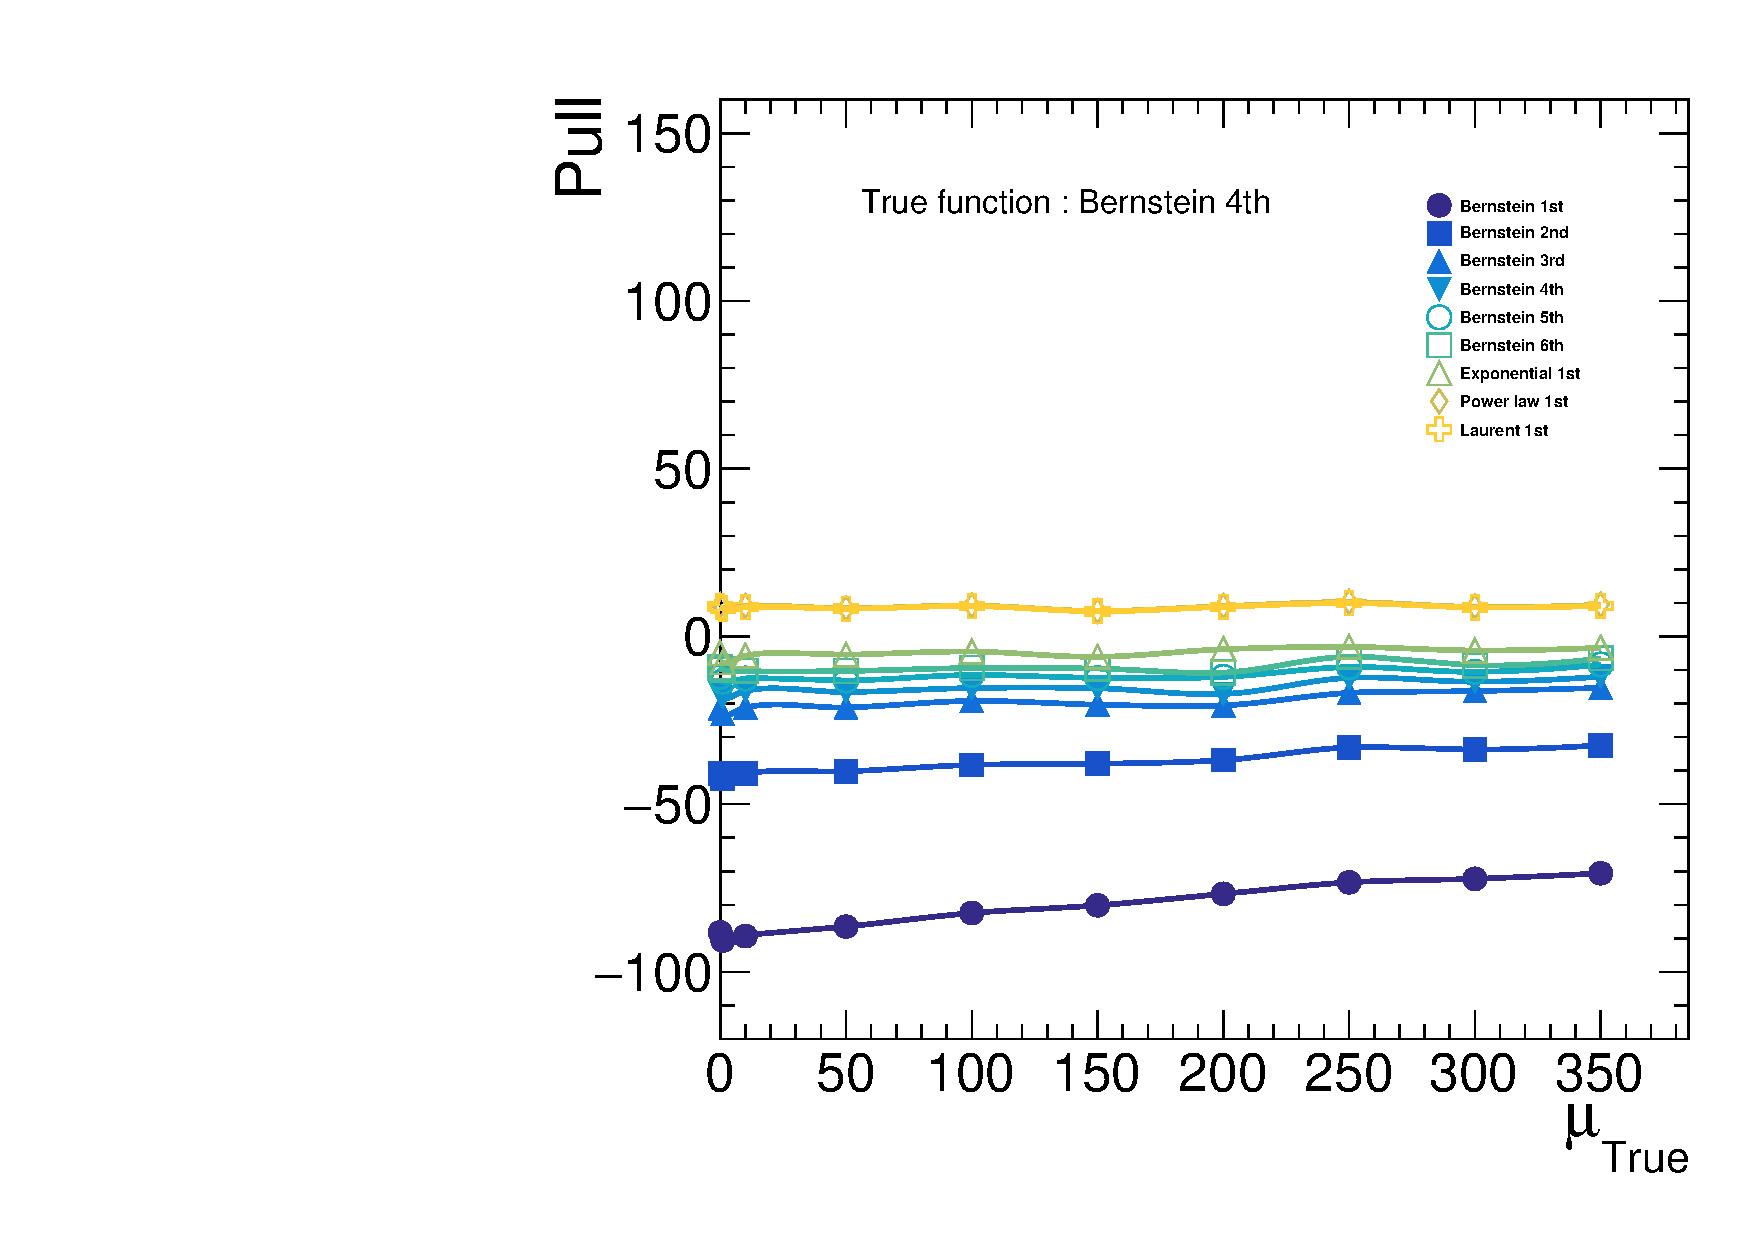
\includegraphics[width=0.33\textwidth]{Fig/BiasStudy/Linearity/HJpsiG/pull_mean_linearity_TrueFunc3}~
  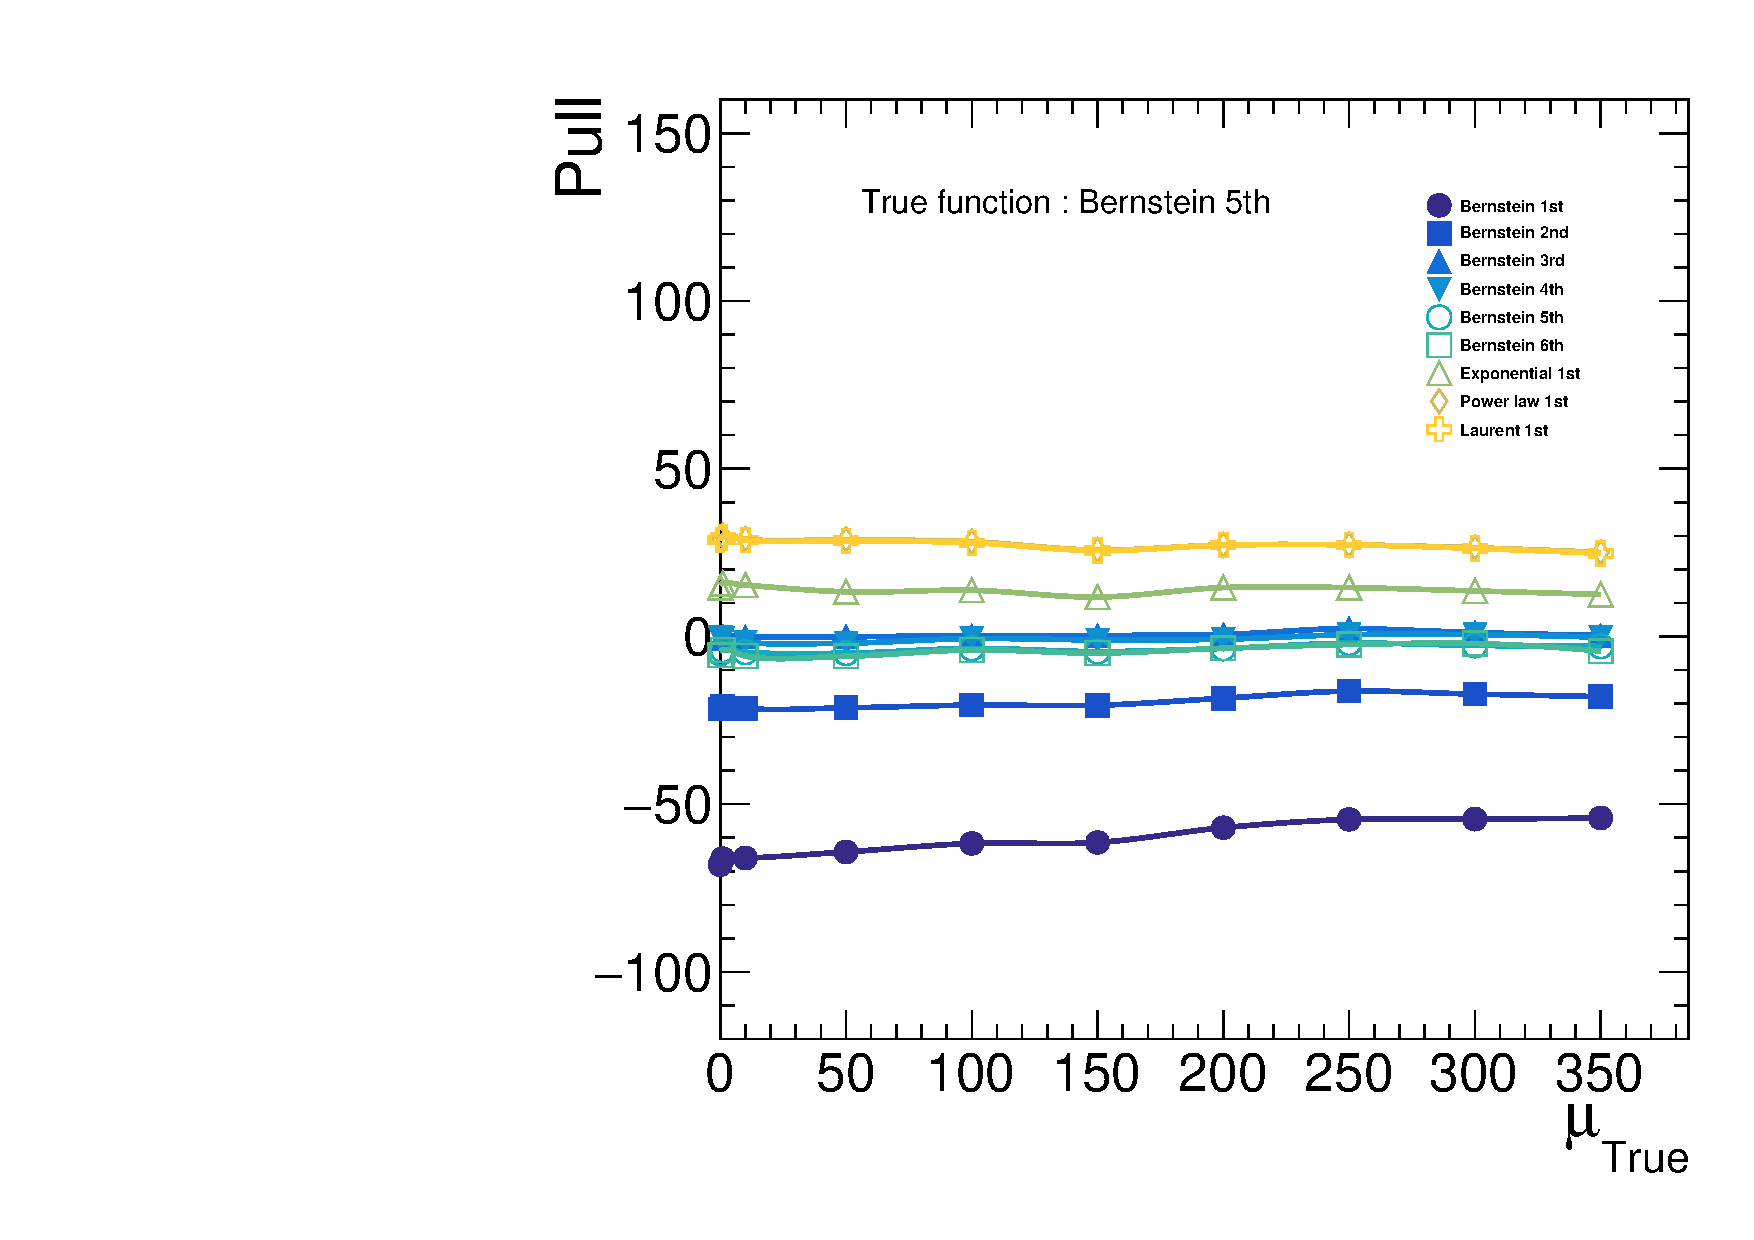
\includegraphics[width=0.33\textwidth]{Fig/BiasStudy/Linearity/HJpsiG/pull_mean_linearity_TrueFunc4}~
  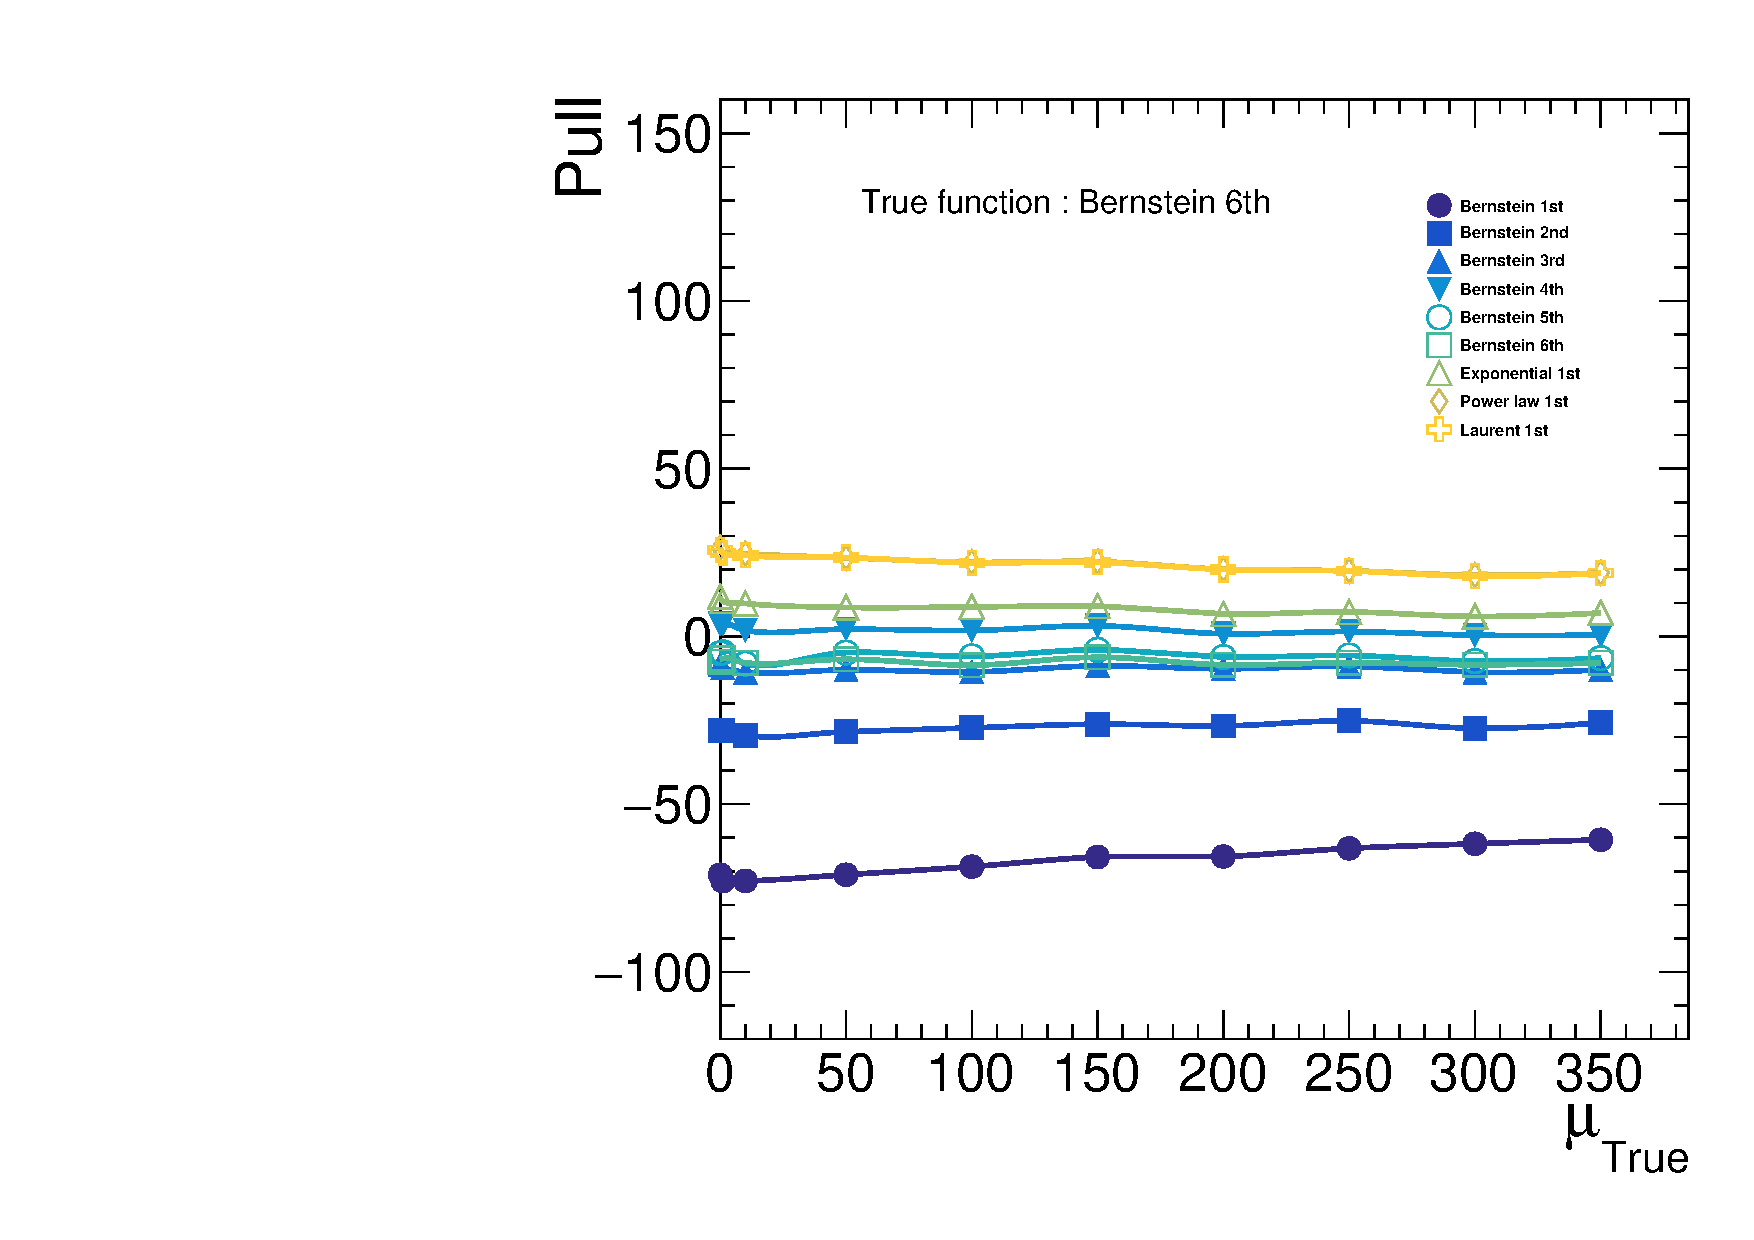
\includegraphics[width=0.33\textwidth]{Fig/BiasStudy/Linearity/HJpsiG/pull_mean_linearity_TrueFunc5}\\
  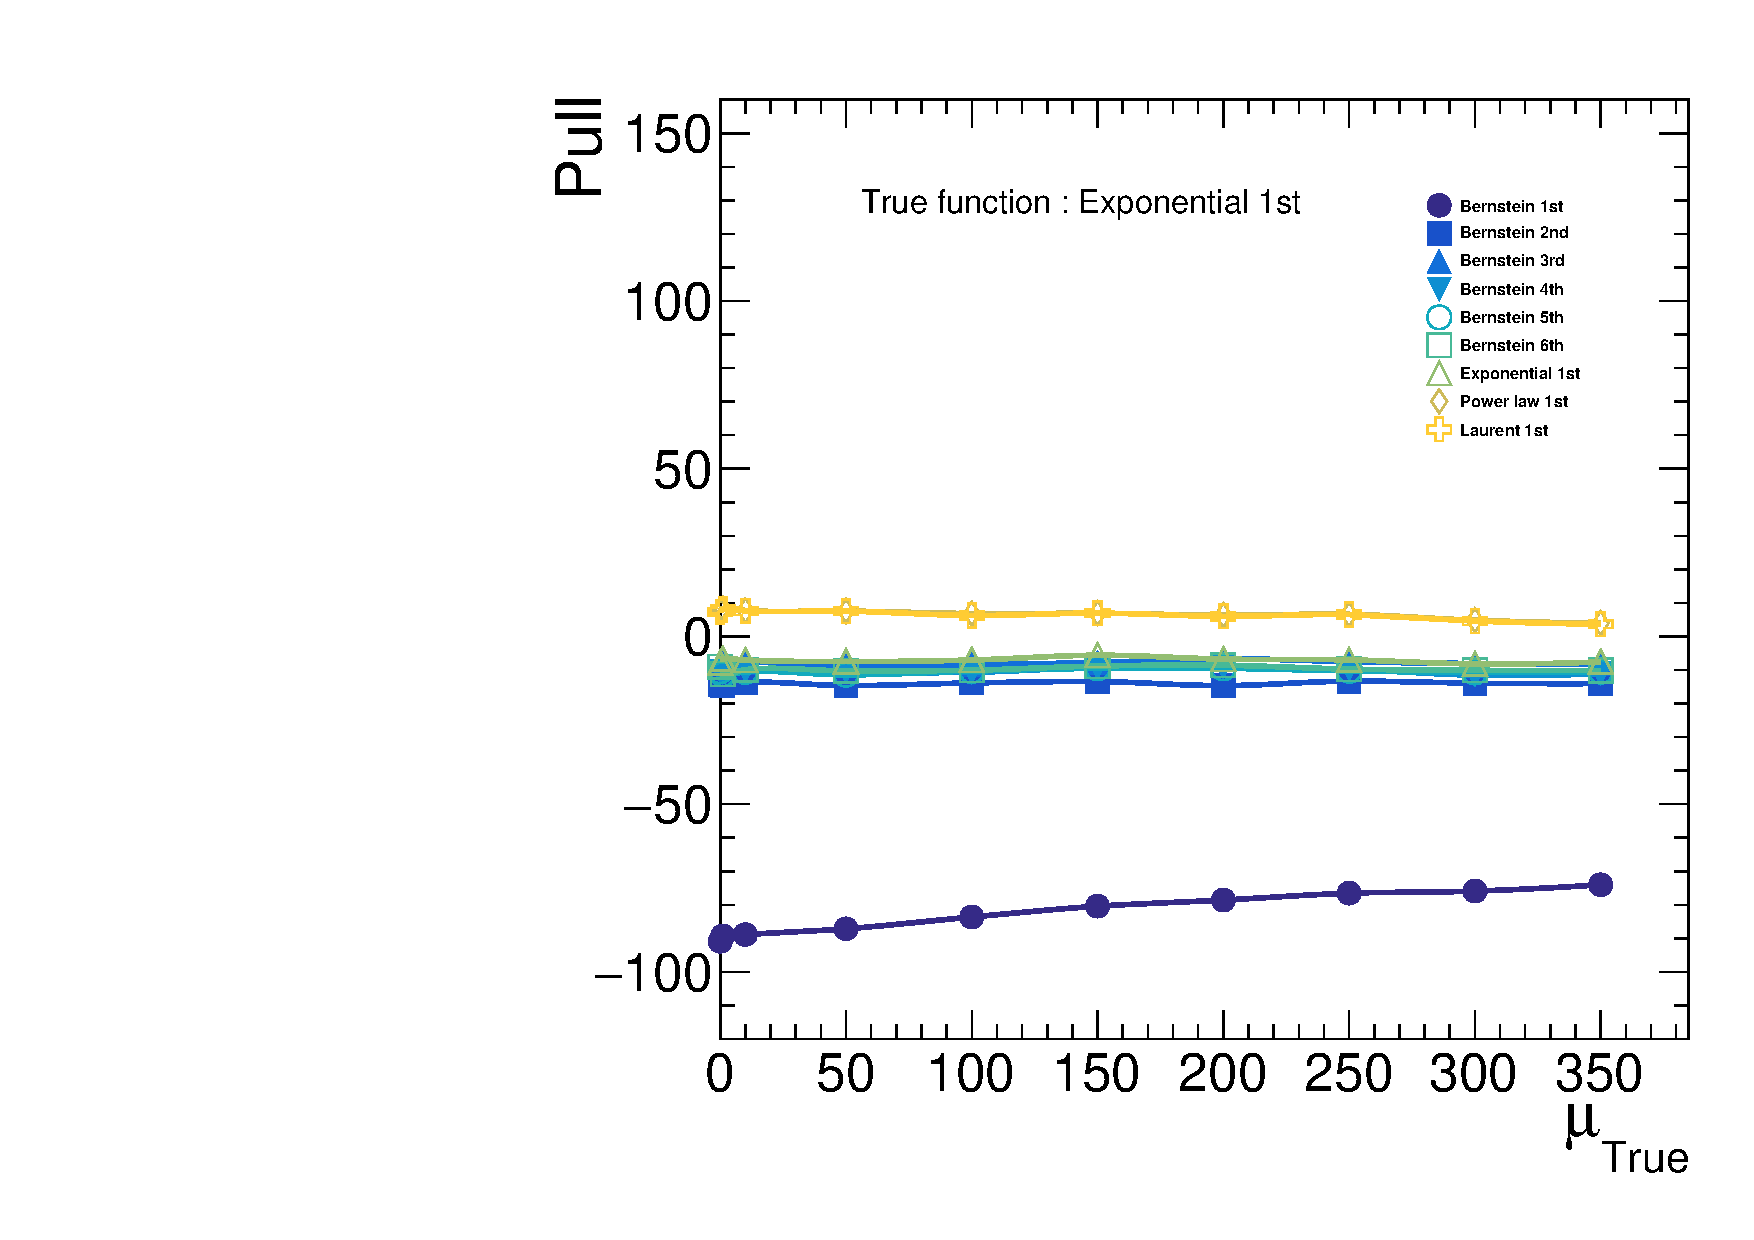
\includegraphics[width=0.33\textwidth]{Fig/BiasStudy/Linearity/HJpsiG/pull_mean_linearity_TrueFunc6}~
  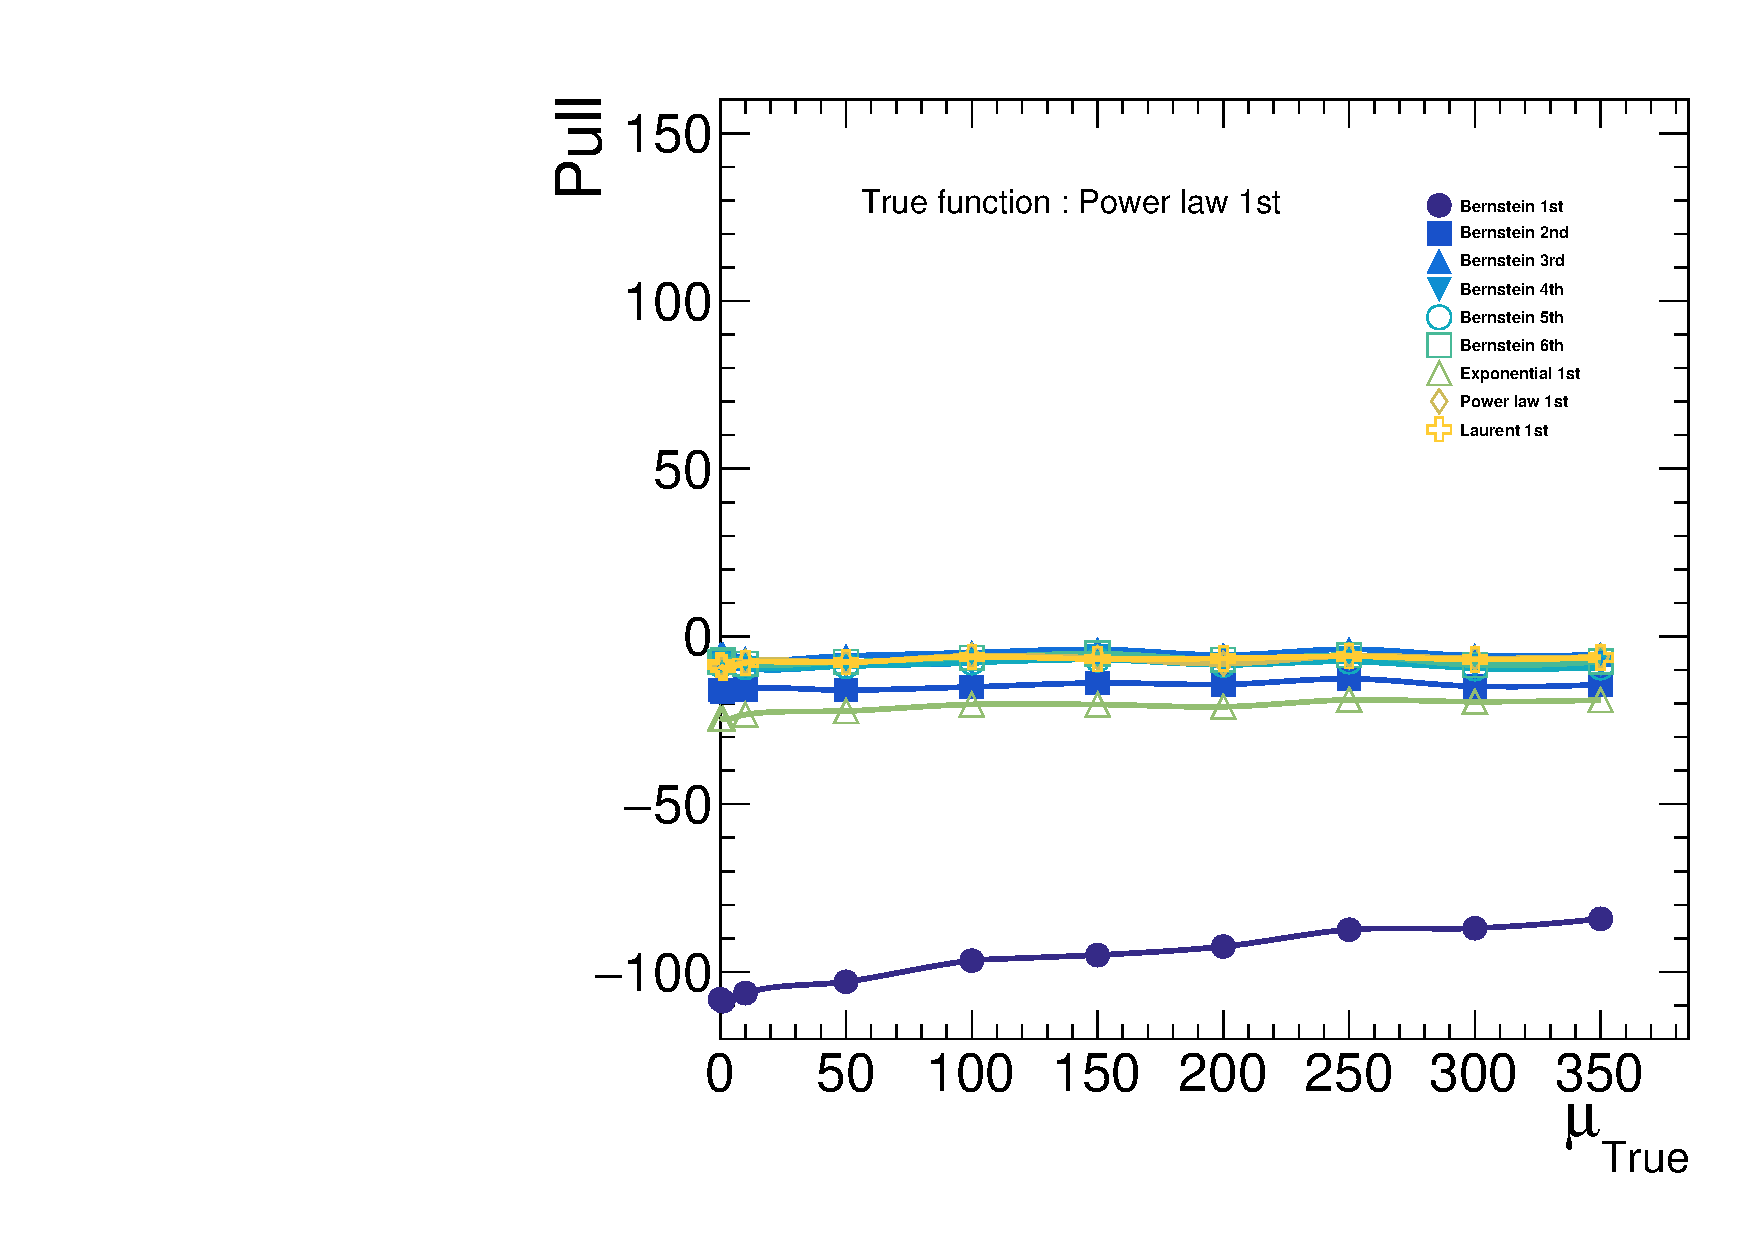
\includegraphics[width=0.33\textwidth]{Fig/BiasStudy/Linearity/HJpsiG/pull_mean_linearity_TrueFunc7}~
  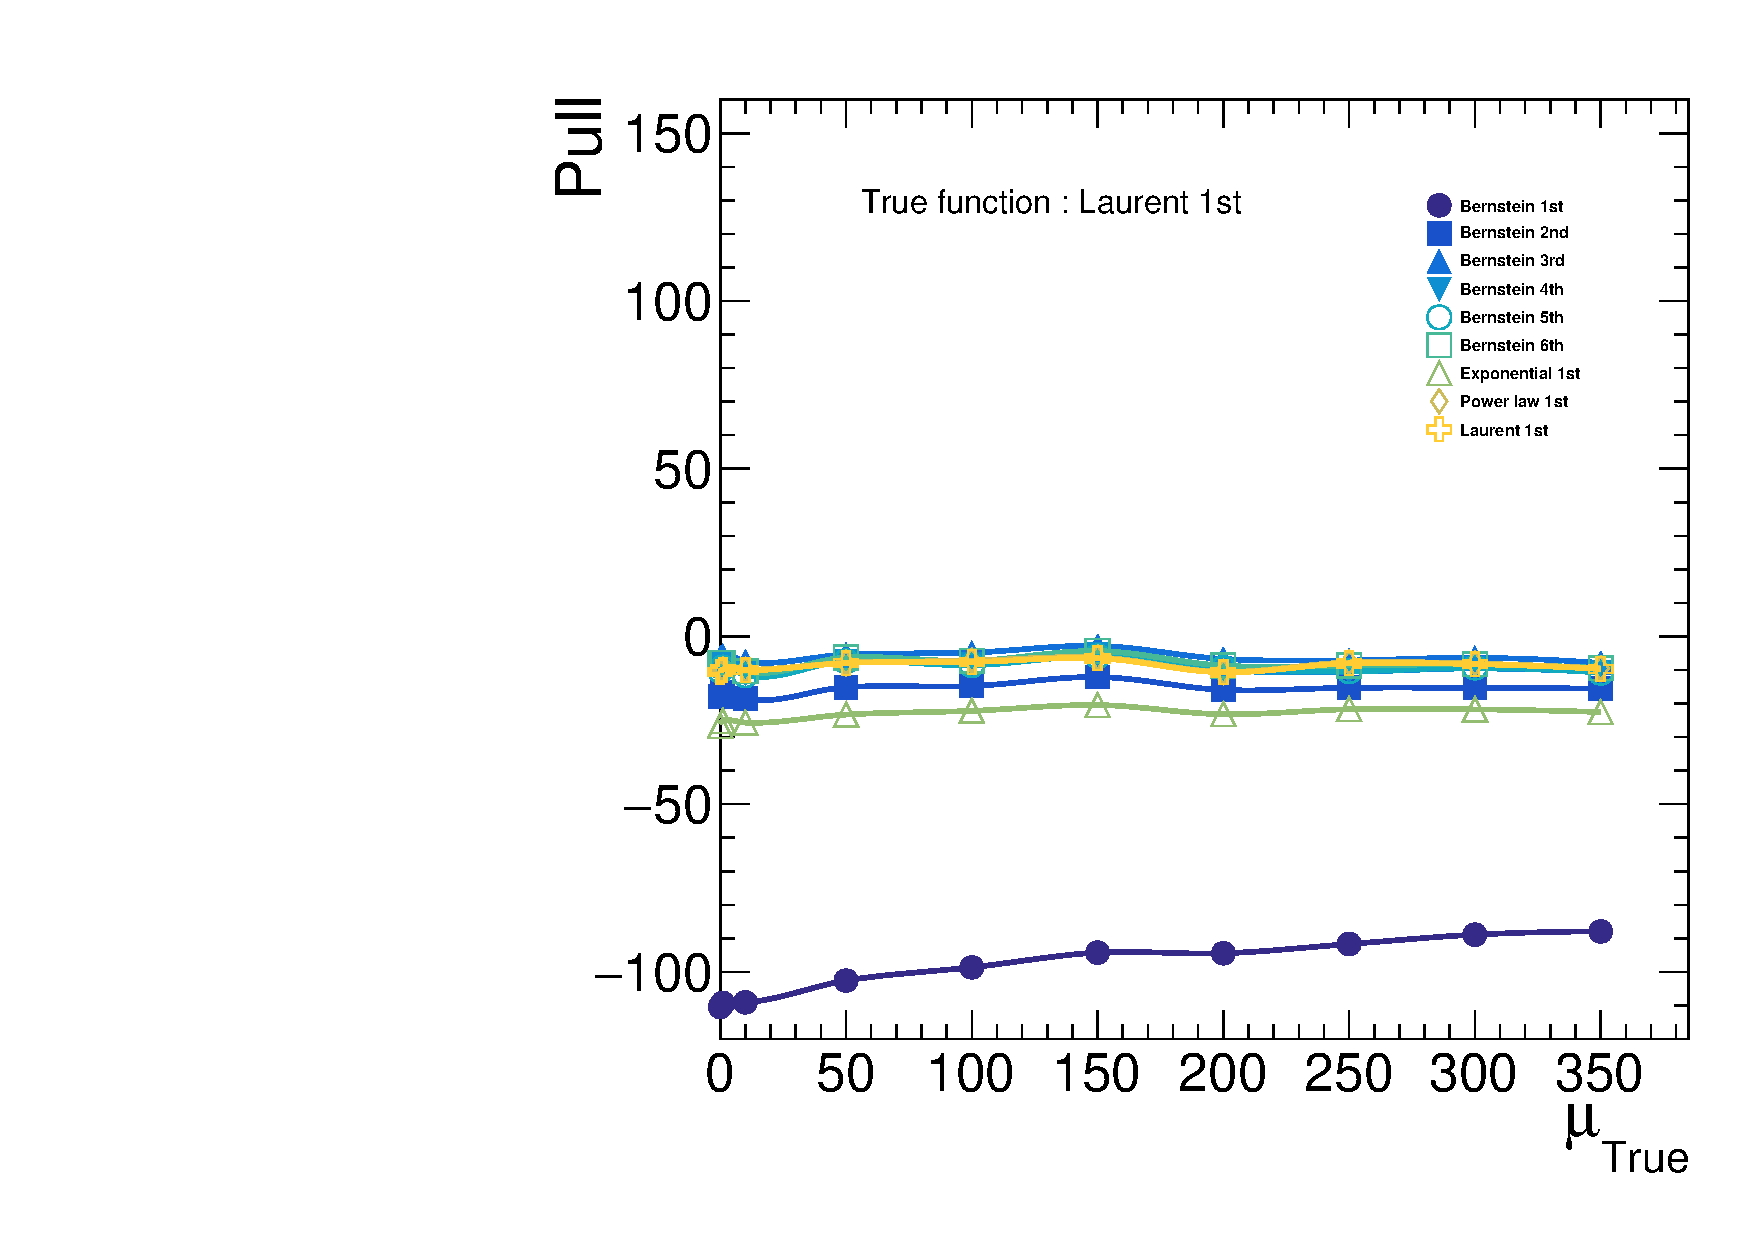
\includegraphics[width=0.33\textwidth]{Fig/BiasStudy/Linearity/HJpsiG/pull_mean_linearity_TrueFunc8}\\
  \caption{The evolution of the mean of the pull value distribution as more signal events are introduced in the Higgs decay.}
  \label{fig:Linearity_mean_HJpsiG}
\end{figure}
\clearpage
\begin{figure}[!ht]
  \centering
  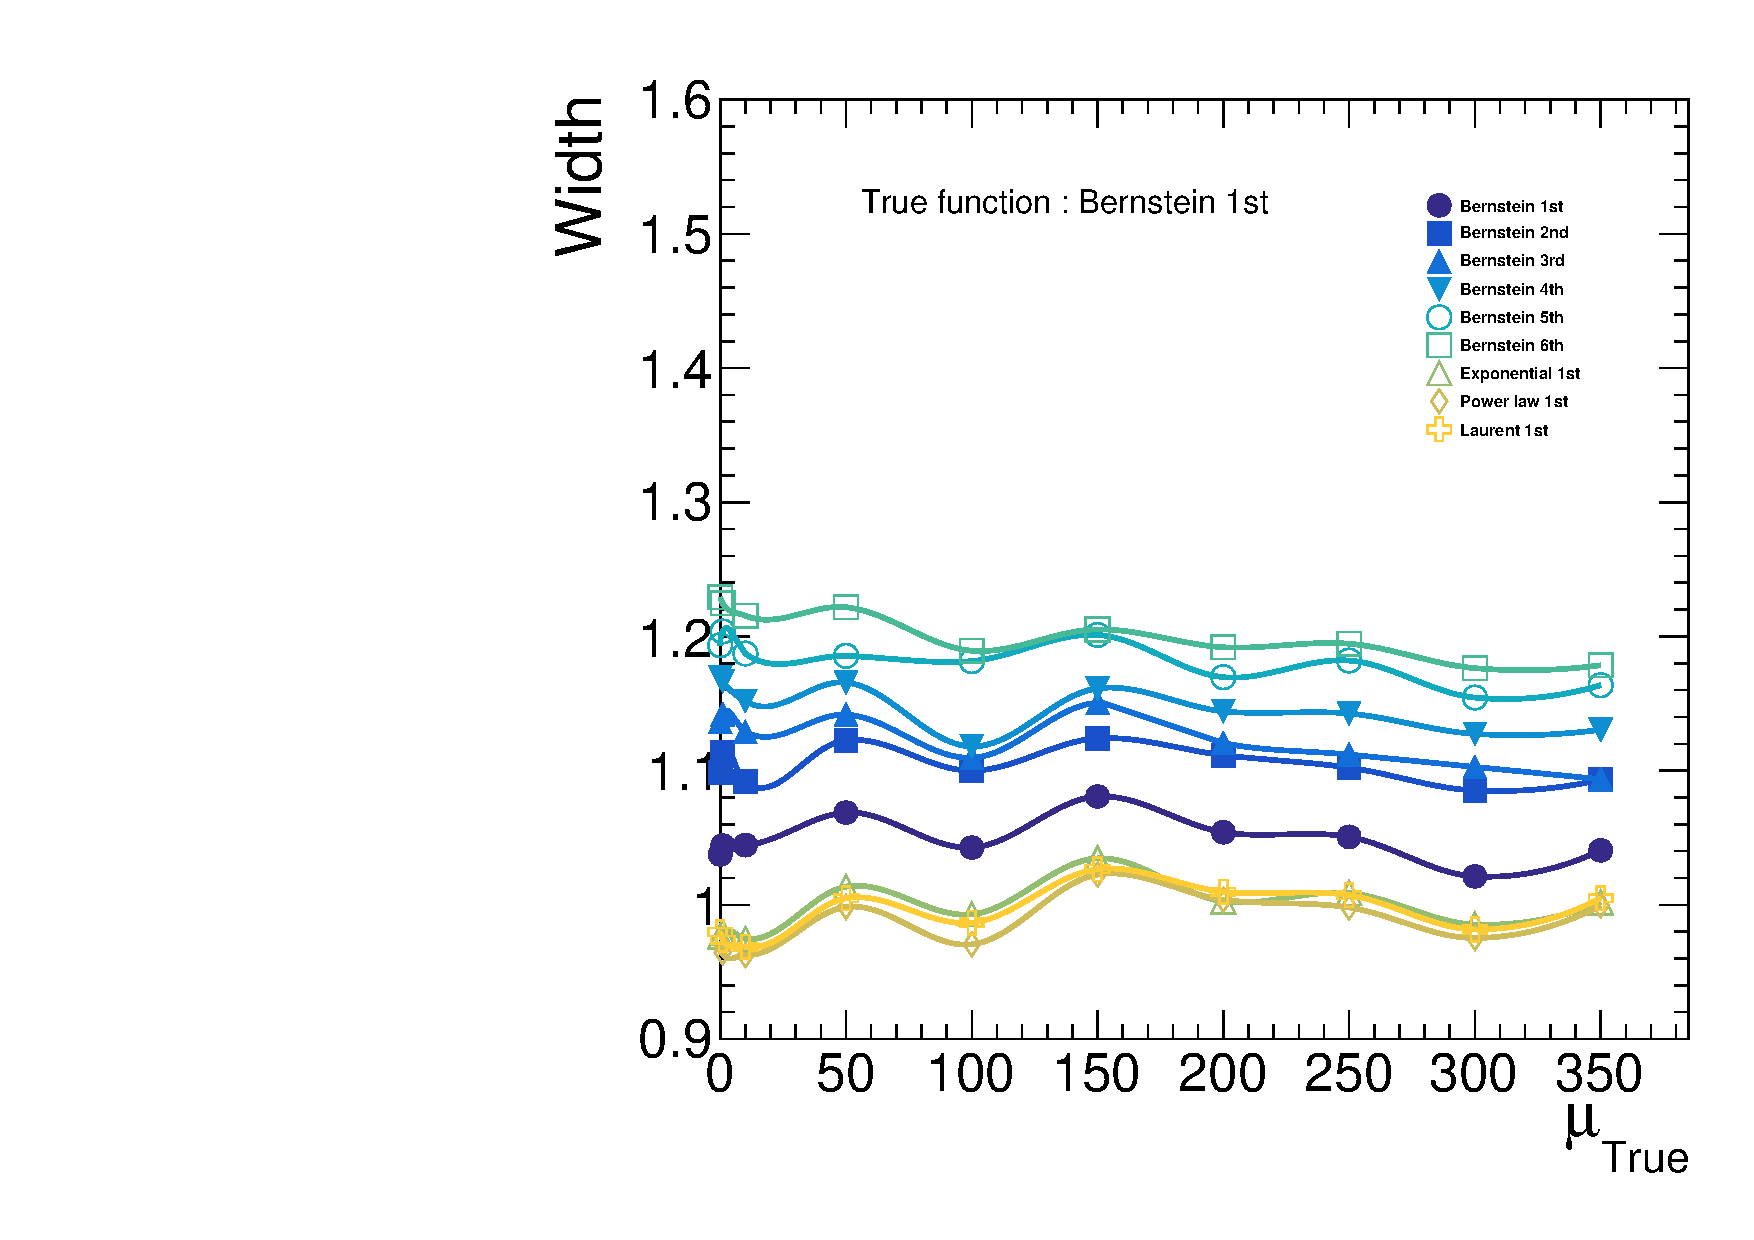
\includegraphics[width=0.33\textwidth]{Fig/BiasStudy/Linearity/HJpsiG/pull_width_linearity_TrueFunc0}~
  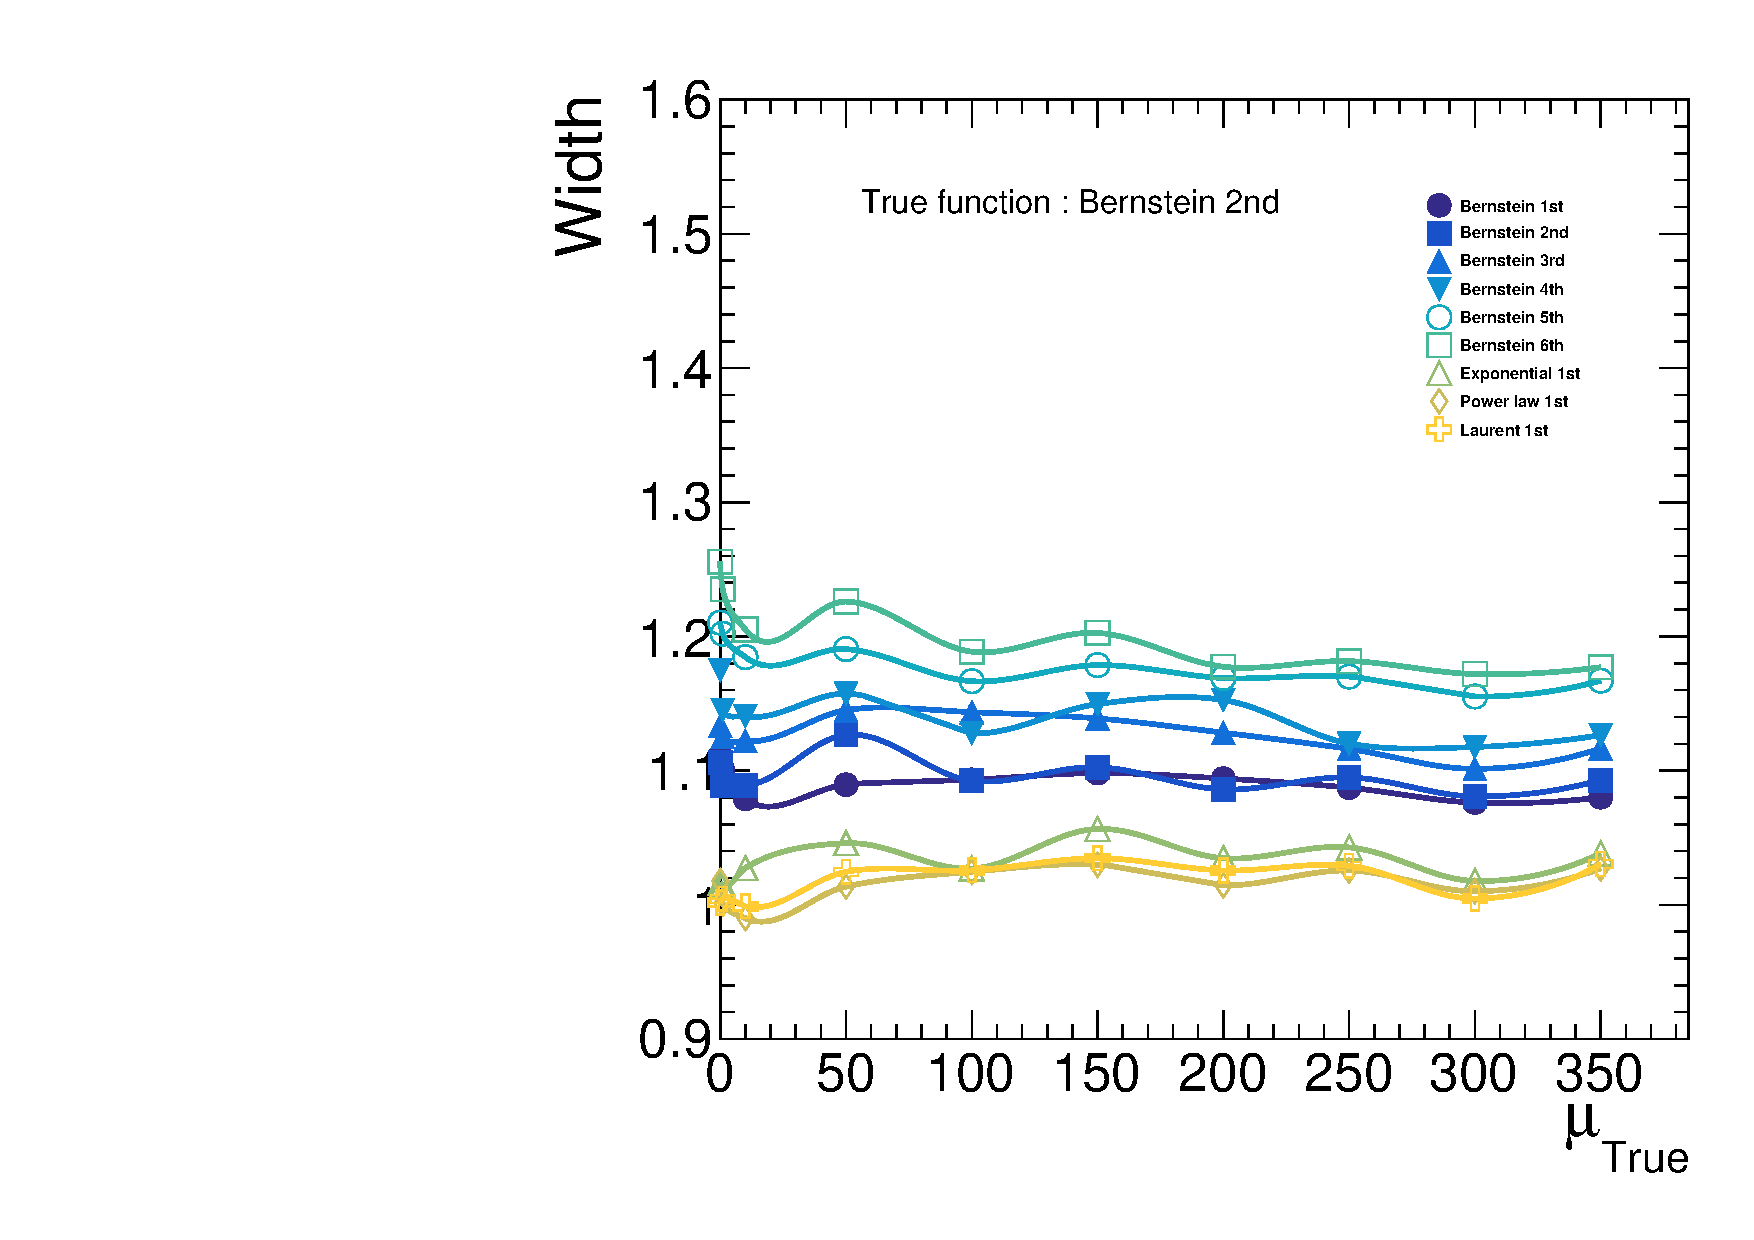
\includegraphics[width=0.33\textwidth]{Fig/BiasStudy/Linearity/HJpsiG/pull_width_linearity_TrueFunc1}~
  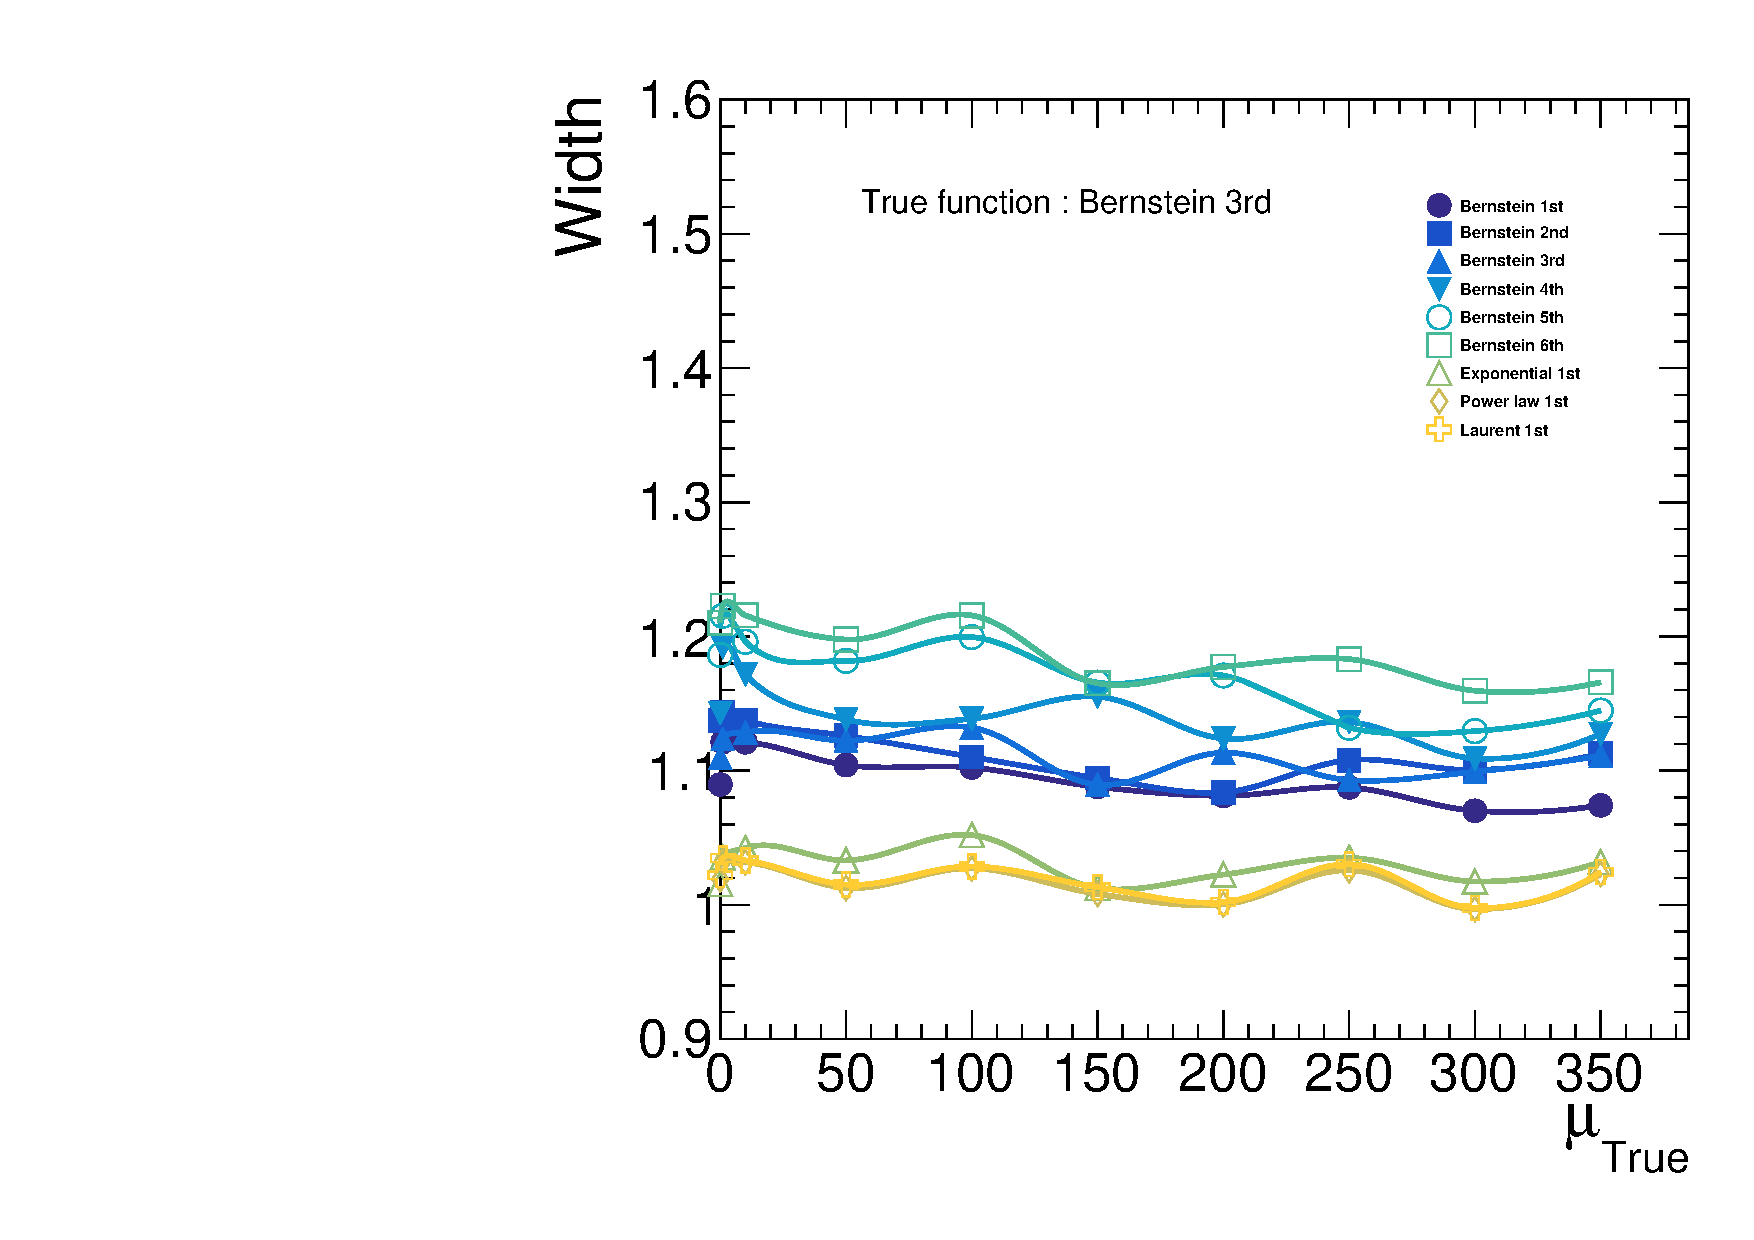
\includegraphics[width=0.33\textwidth]{Fig/BiasStudy/Linearity/HJpsiG/pull_width_linearity_TrueFunc2}\\
  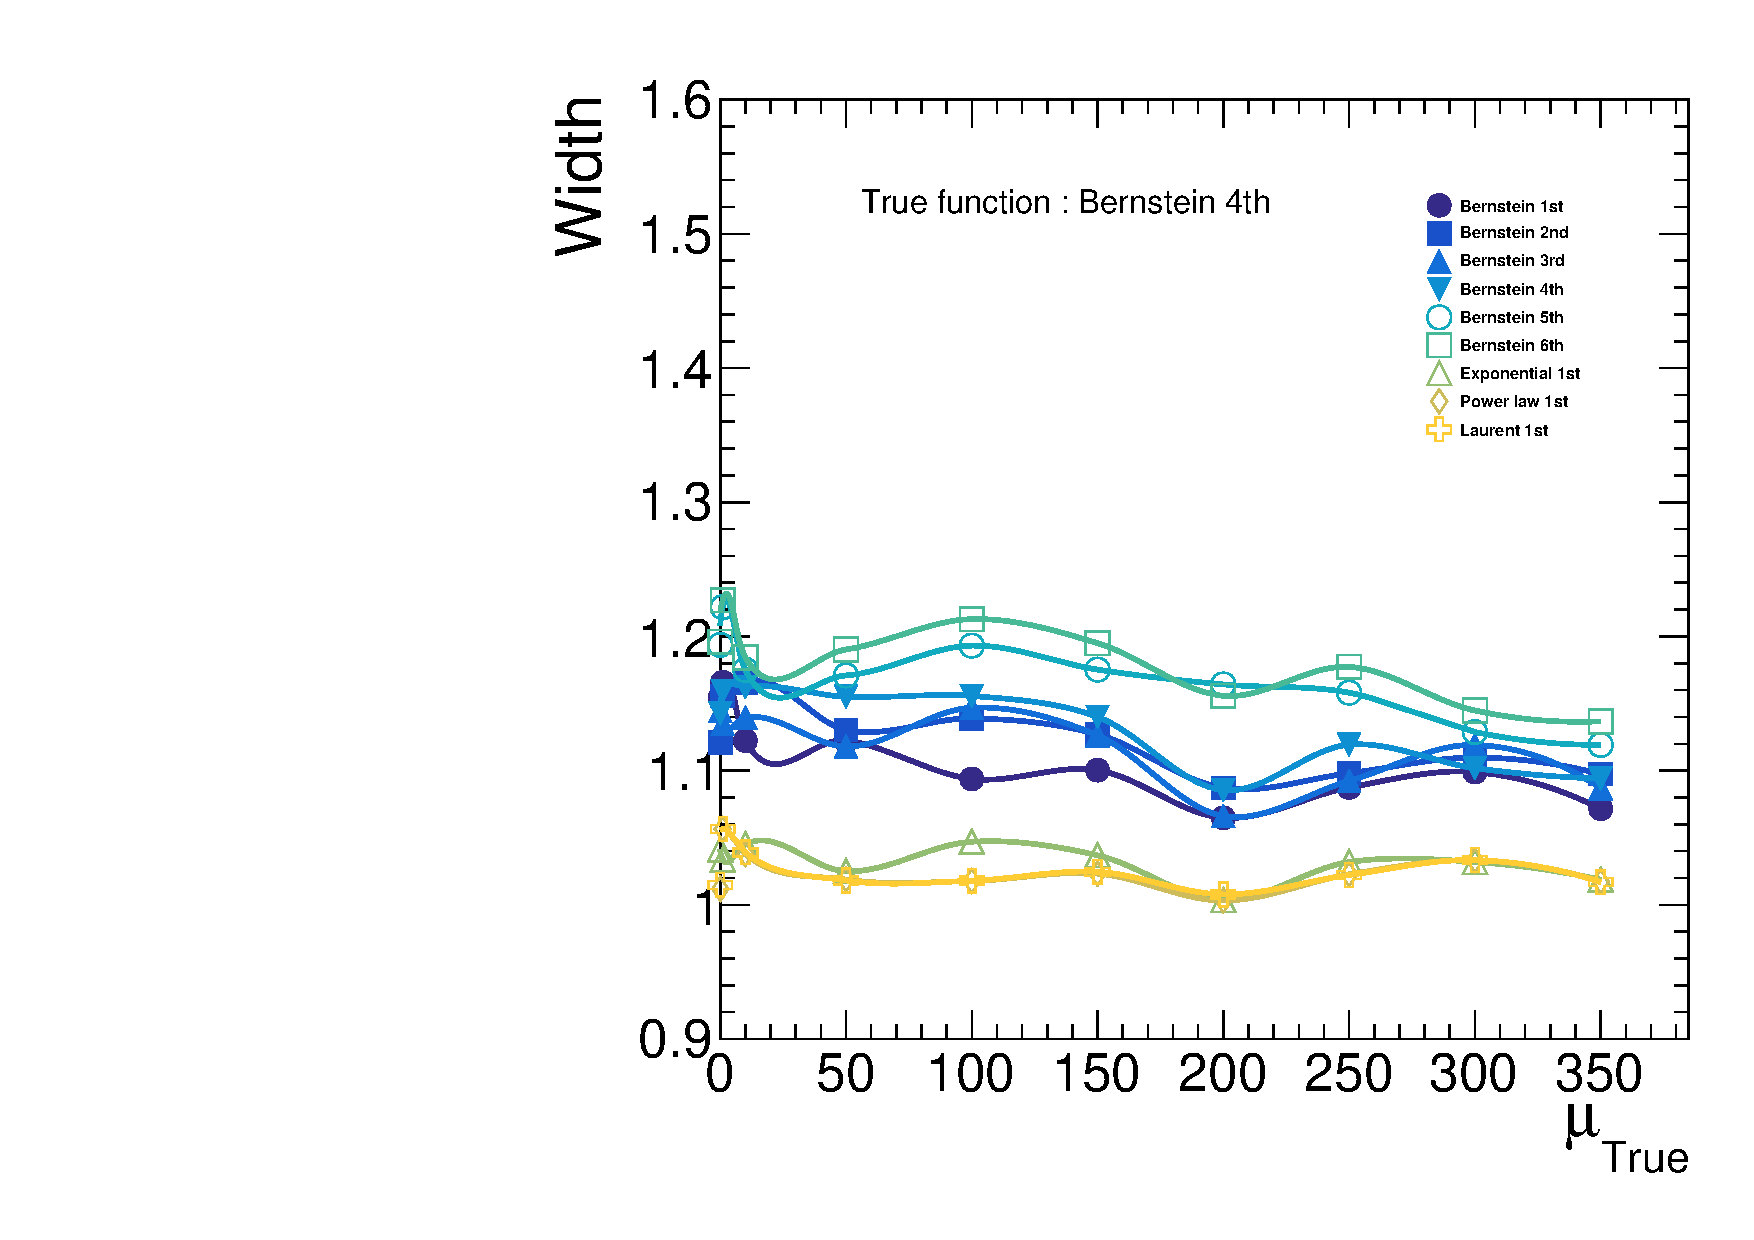
\includegraphics[width=0.33\textwidth]{Fig/BiasStudy/Linearity/HJpsiG/pull_width_linearity_TrueFunc3}~
  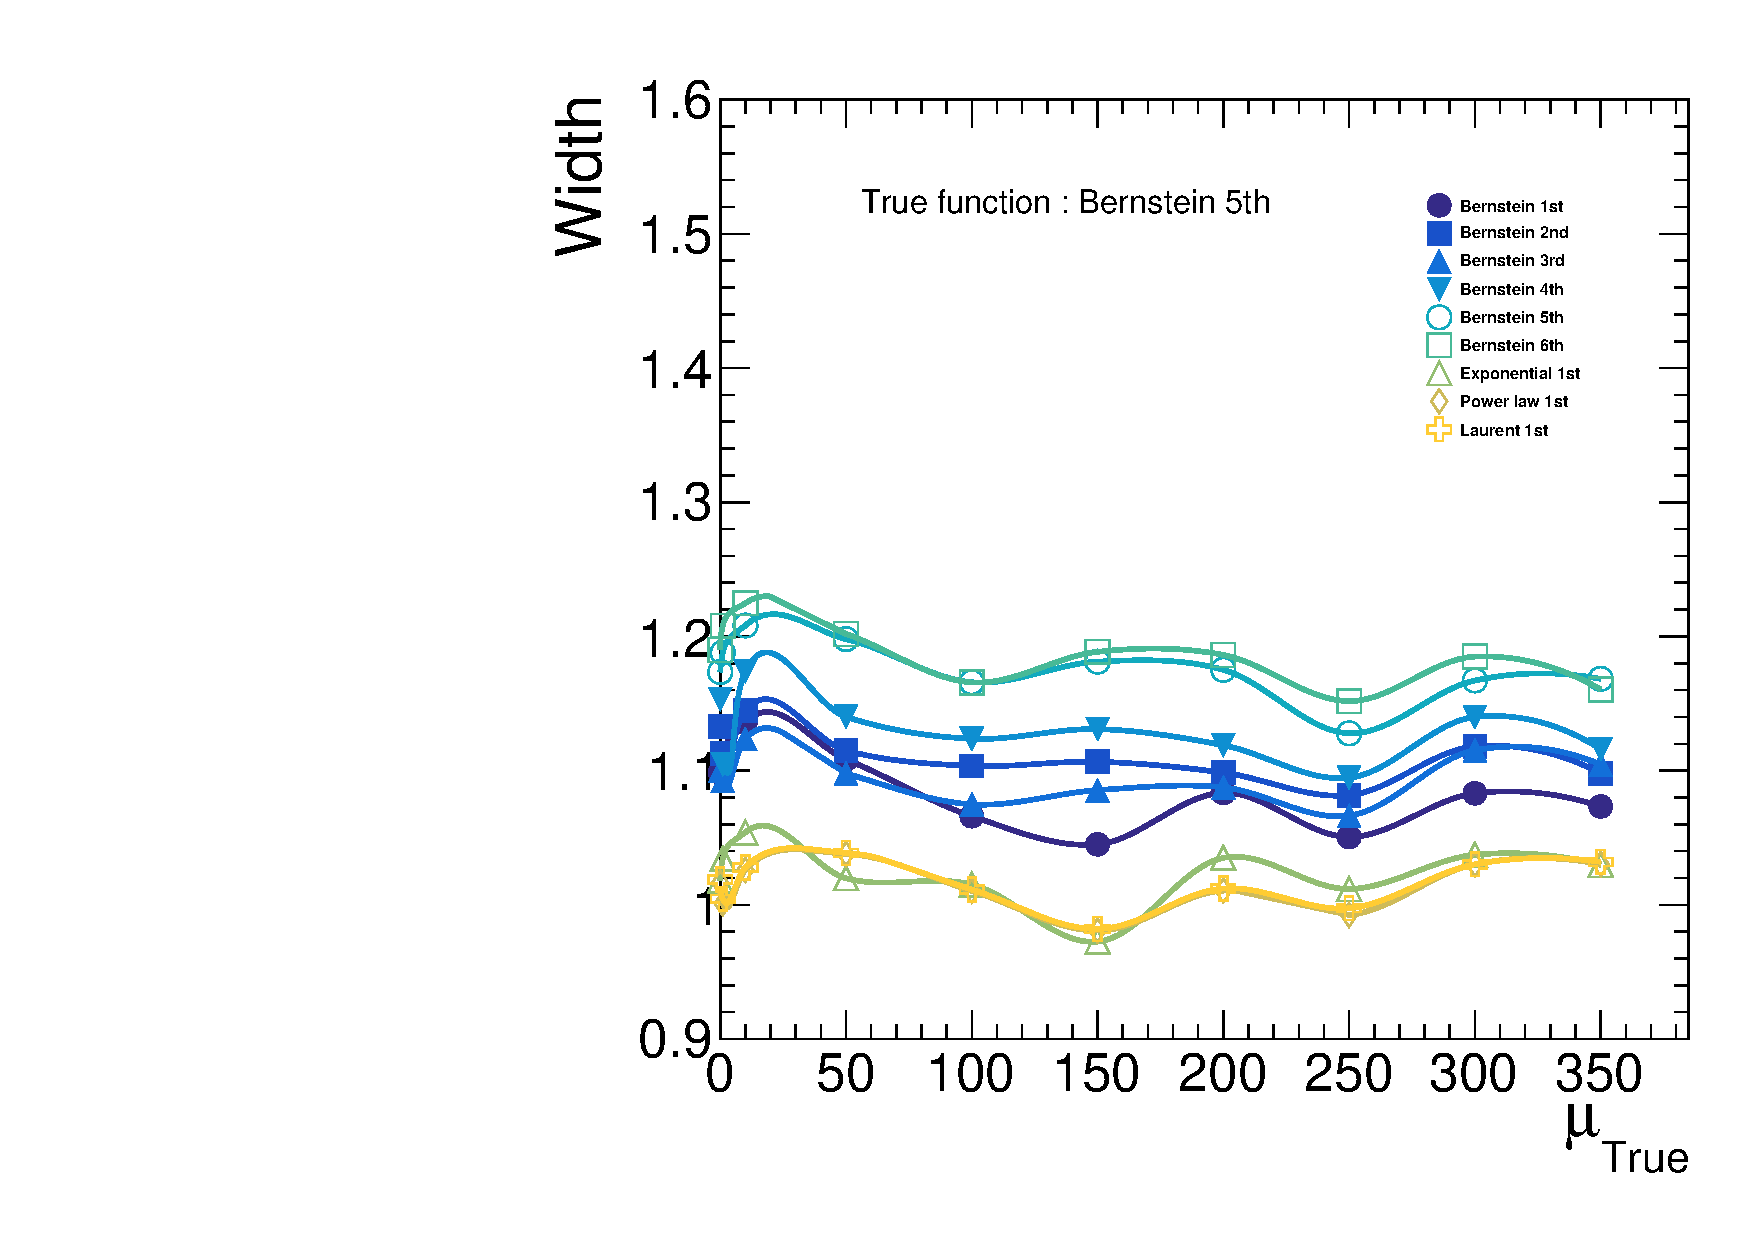
\includegraphics[width=0.33\textwidth]{Fig/BiasStudy/Linearity/HJpsiG/pull_width_linearity_TrueFunc4}~
  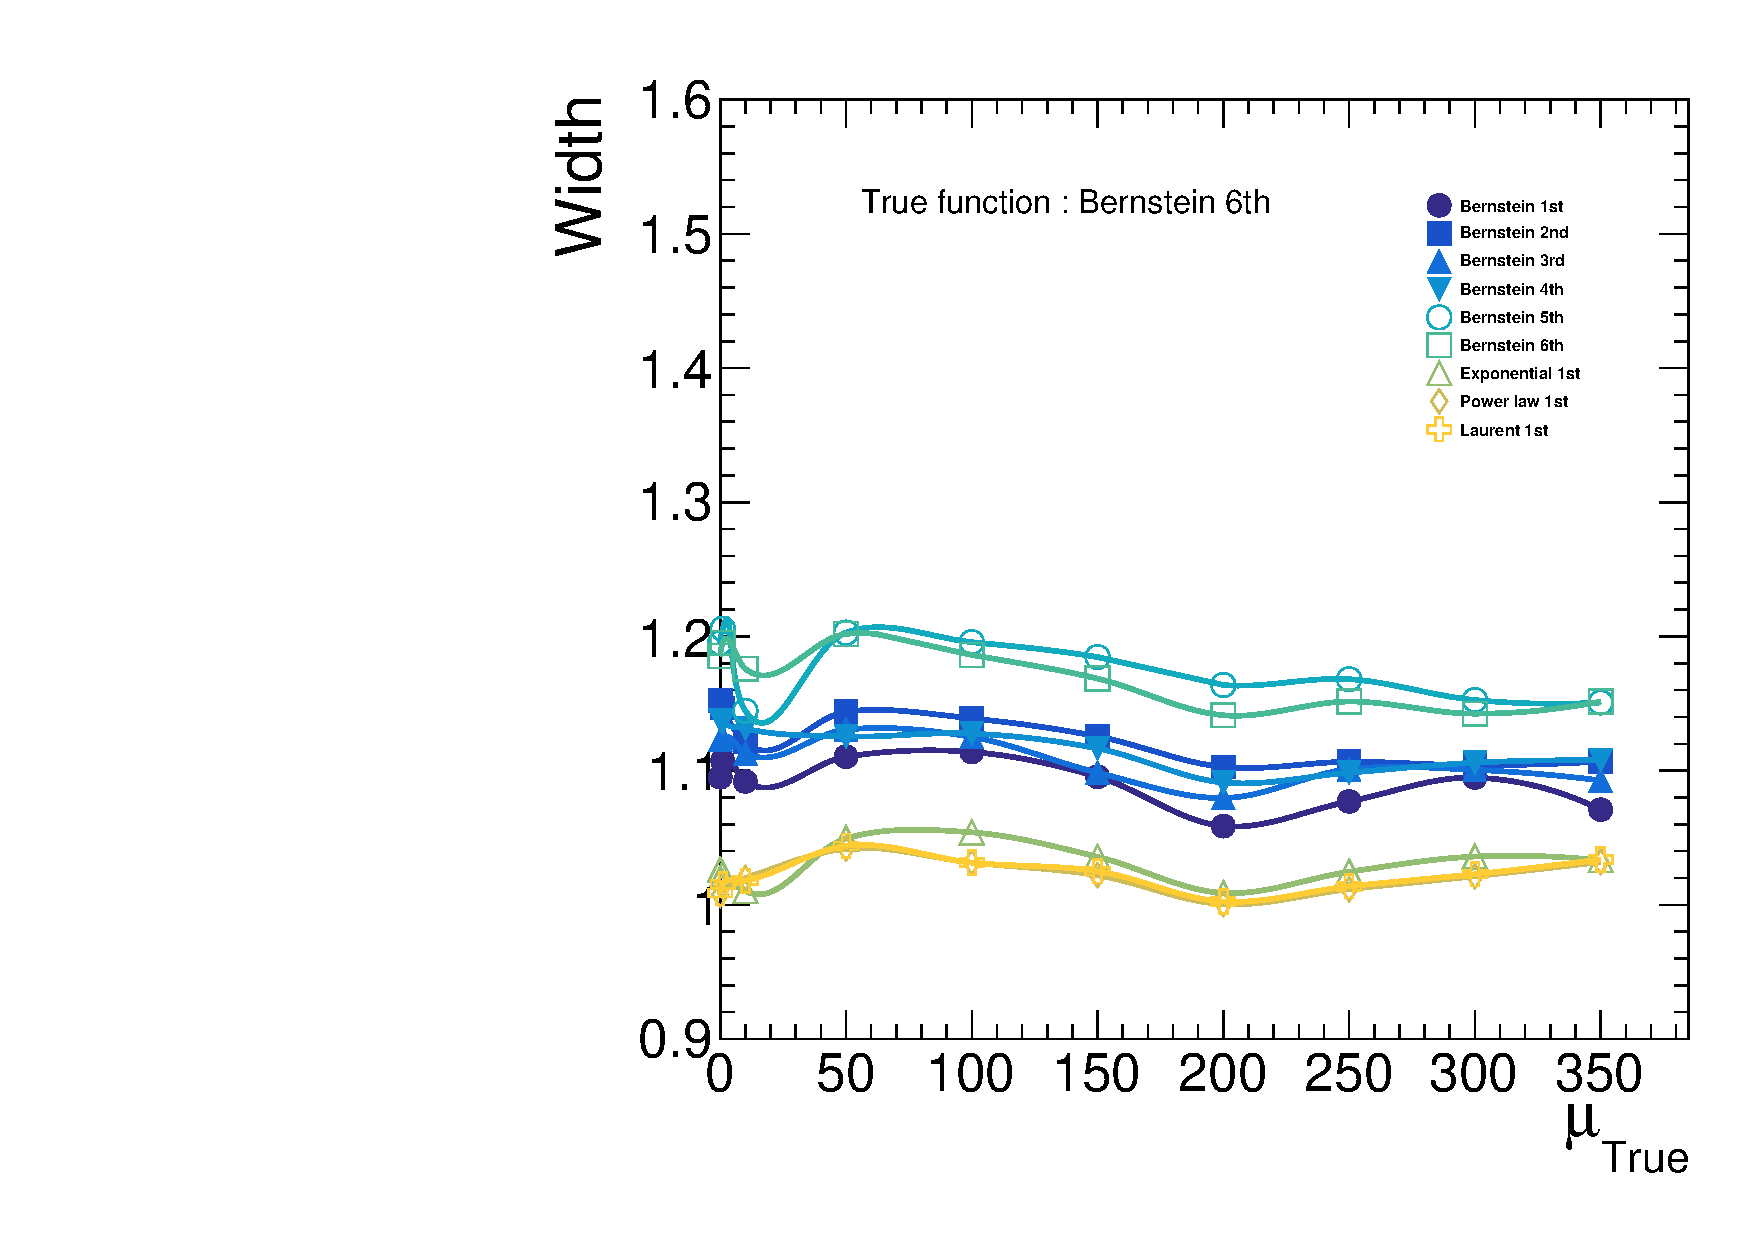
\includegraphics[width=0.33\textwidth]{Fig/BiasStudy/Linearity/HJpsiG/pull_width_linearity_TrueFunc5}\\
  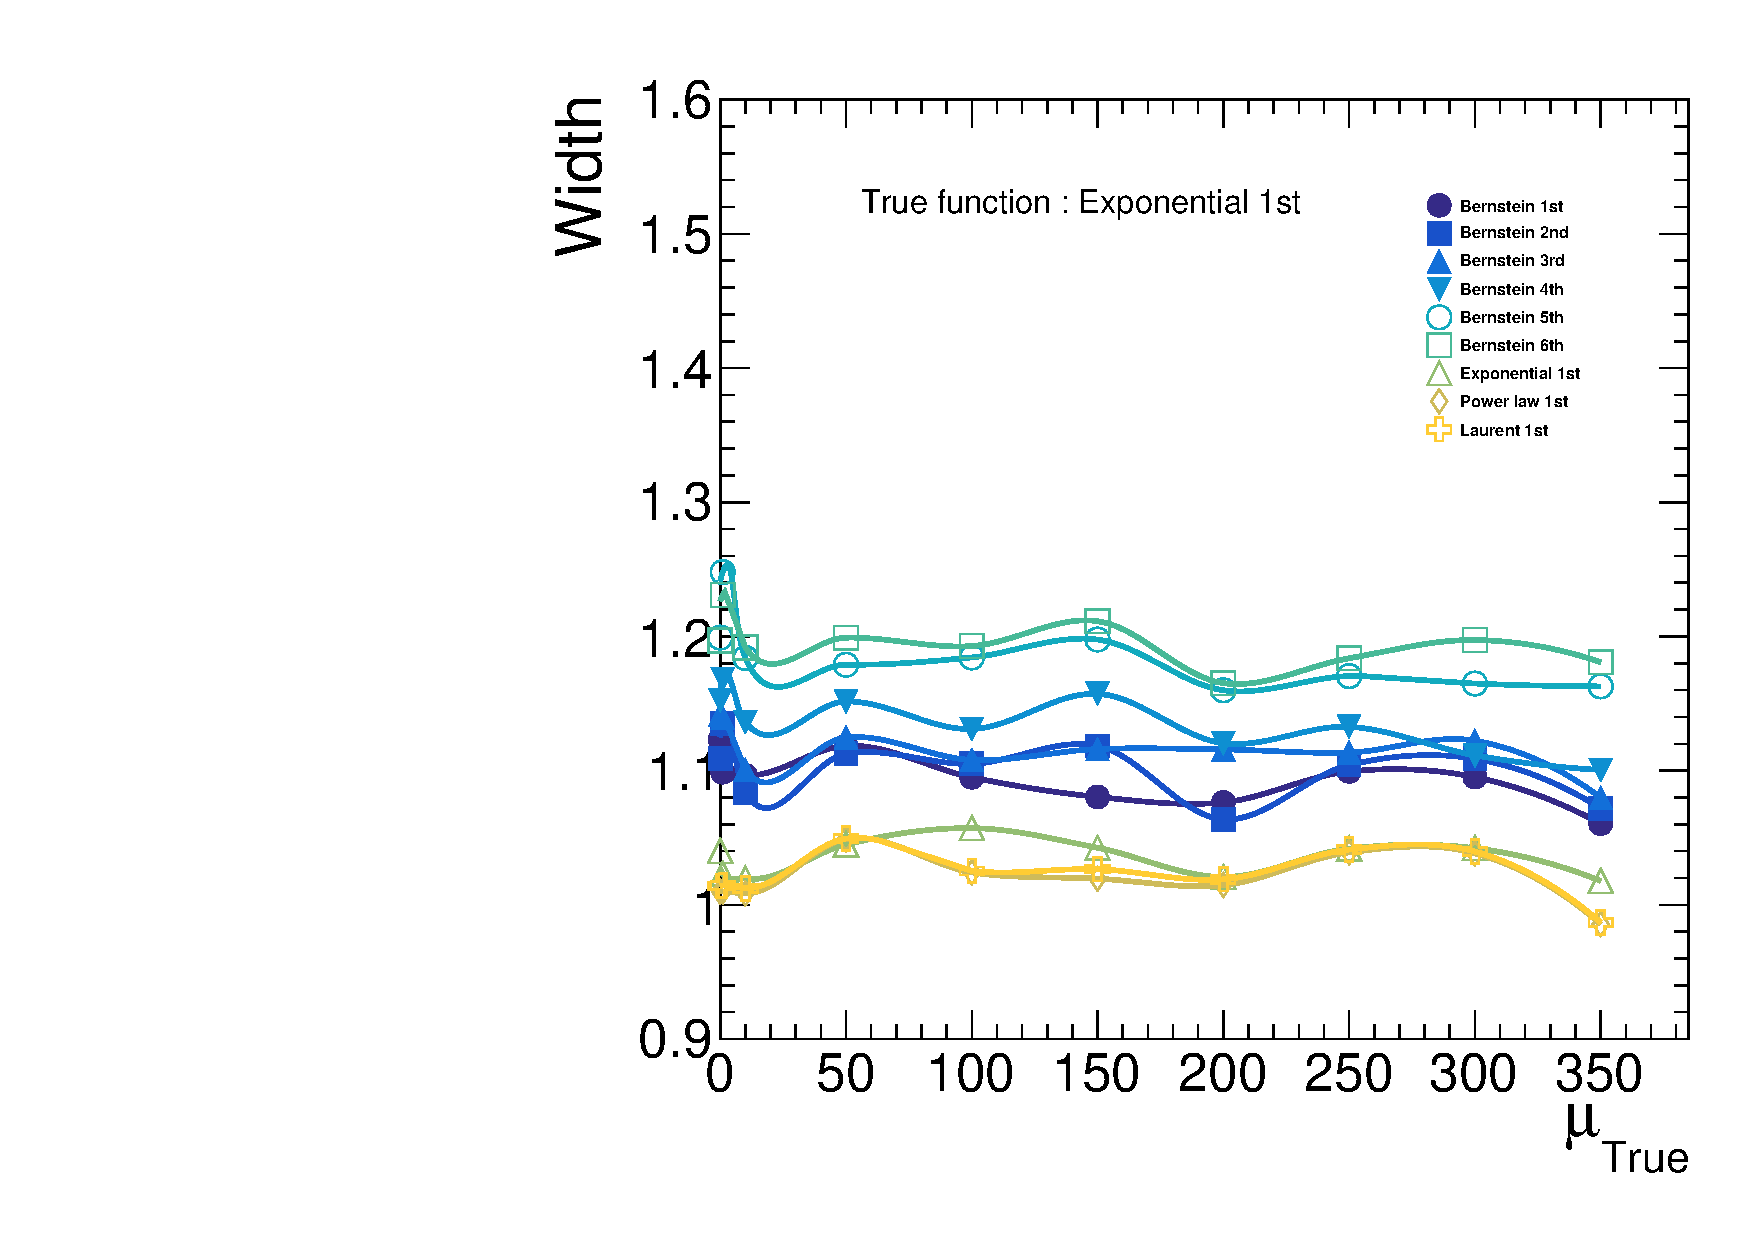
\includegraphics[width=0.33\textwidth]{Fig/BiasStudy/Linearity/HJpsiG/pull_width_linearity_TrueFunc6}~
  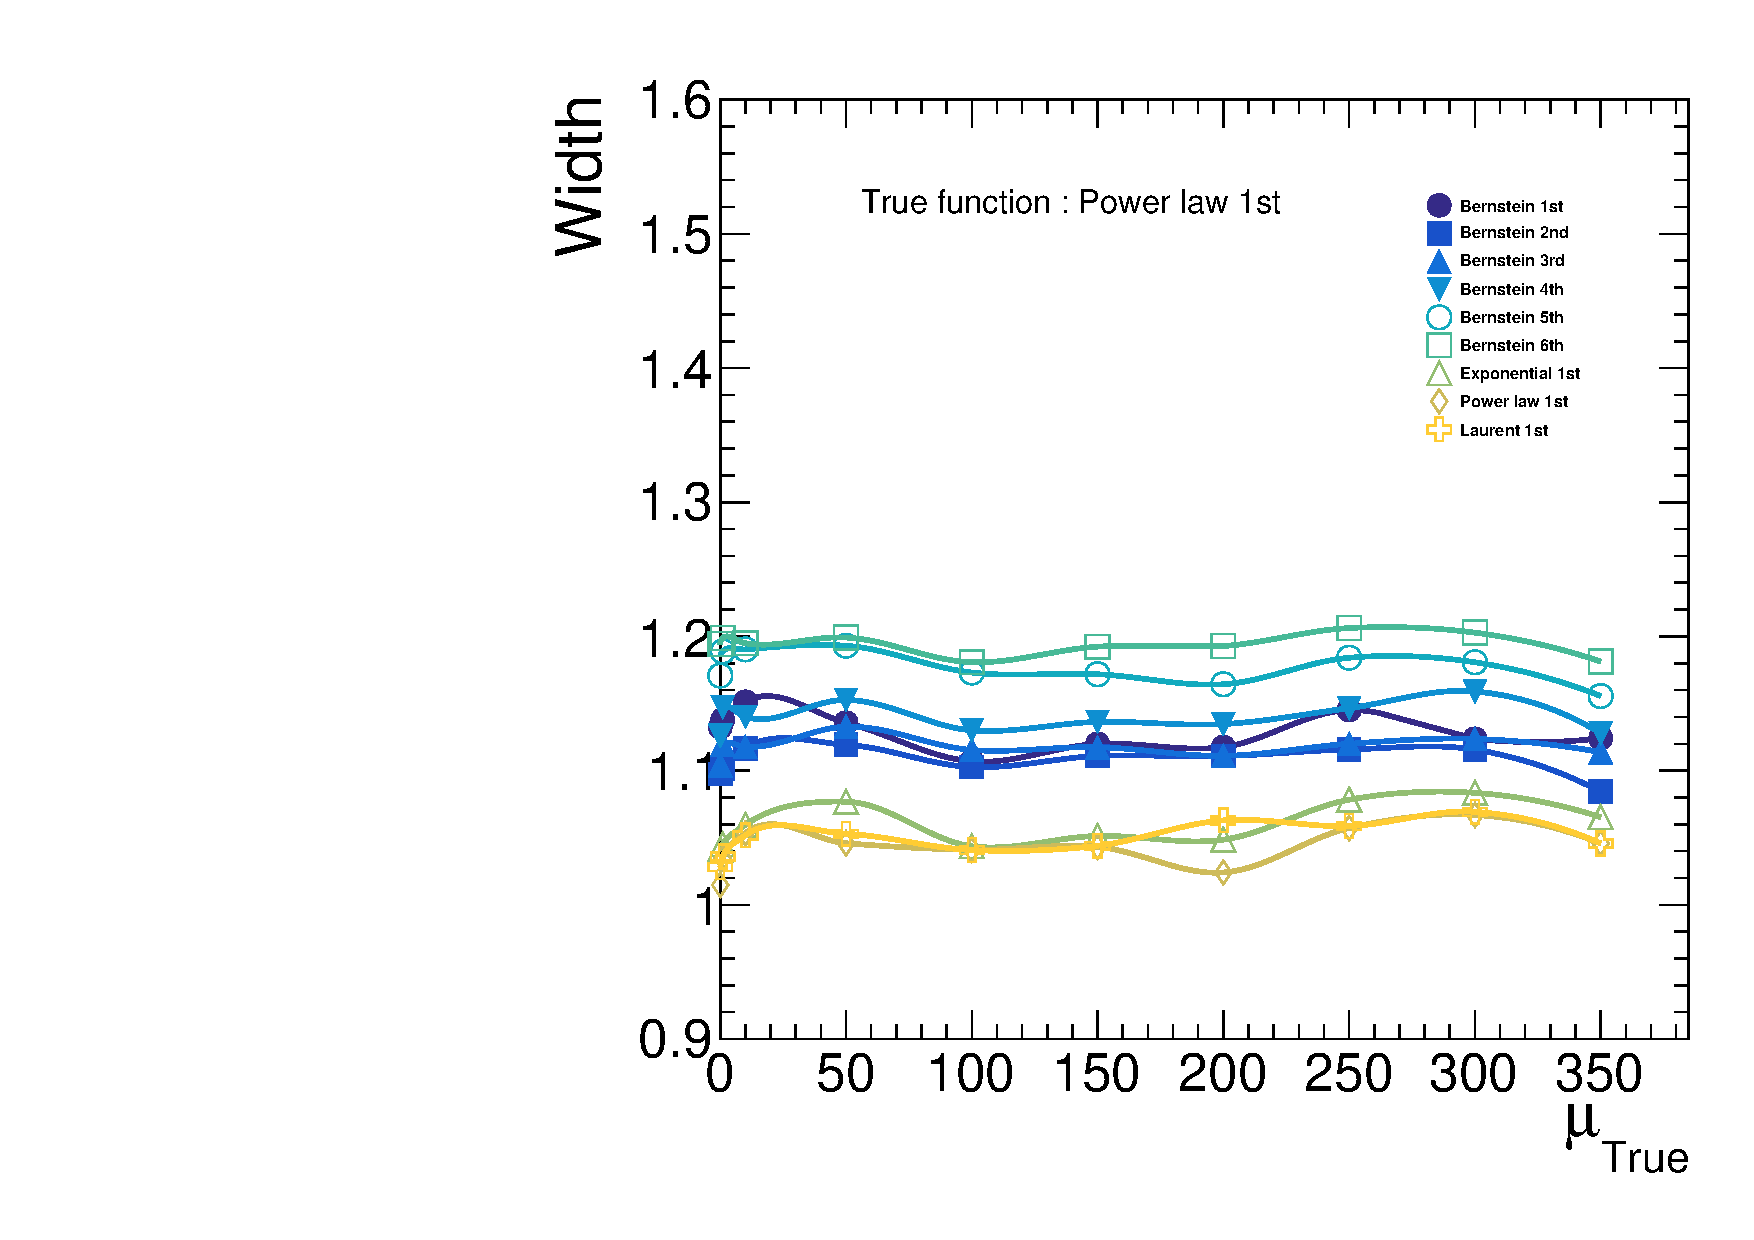
\includegraphics[width=0.33\textwidth]{Fig/BiasStudy/Linearity/HJpsiG/pull_width_linearity_TrueFunc7}~
  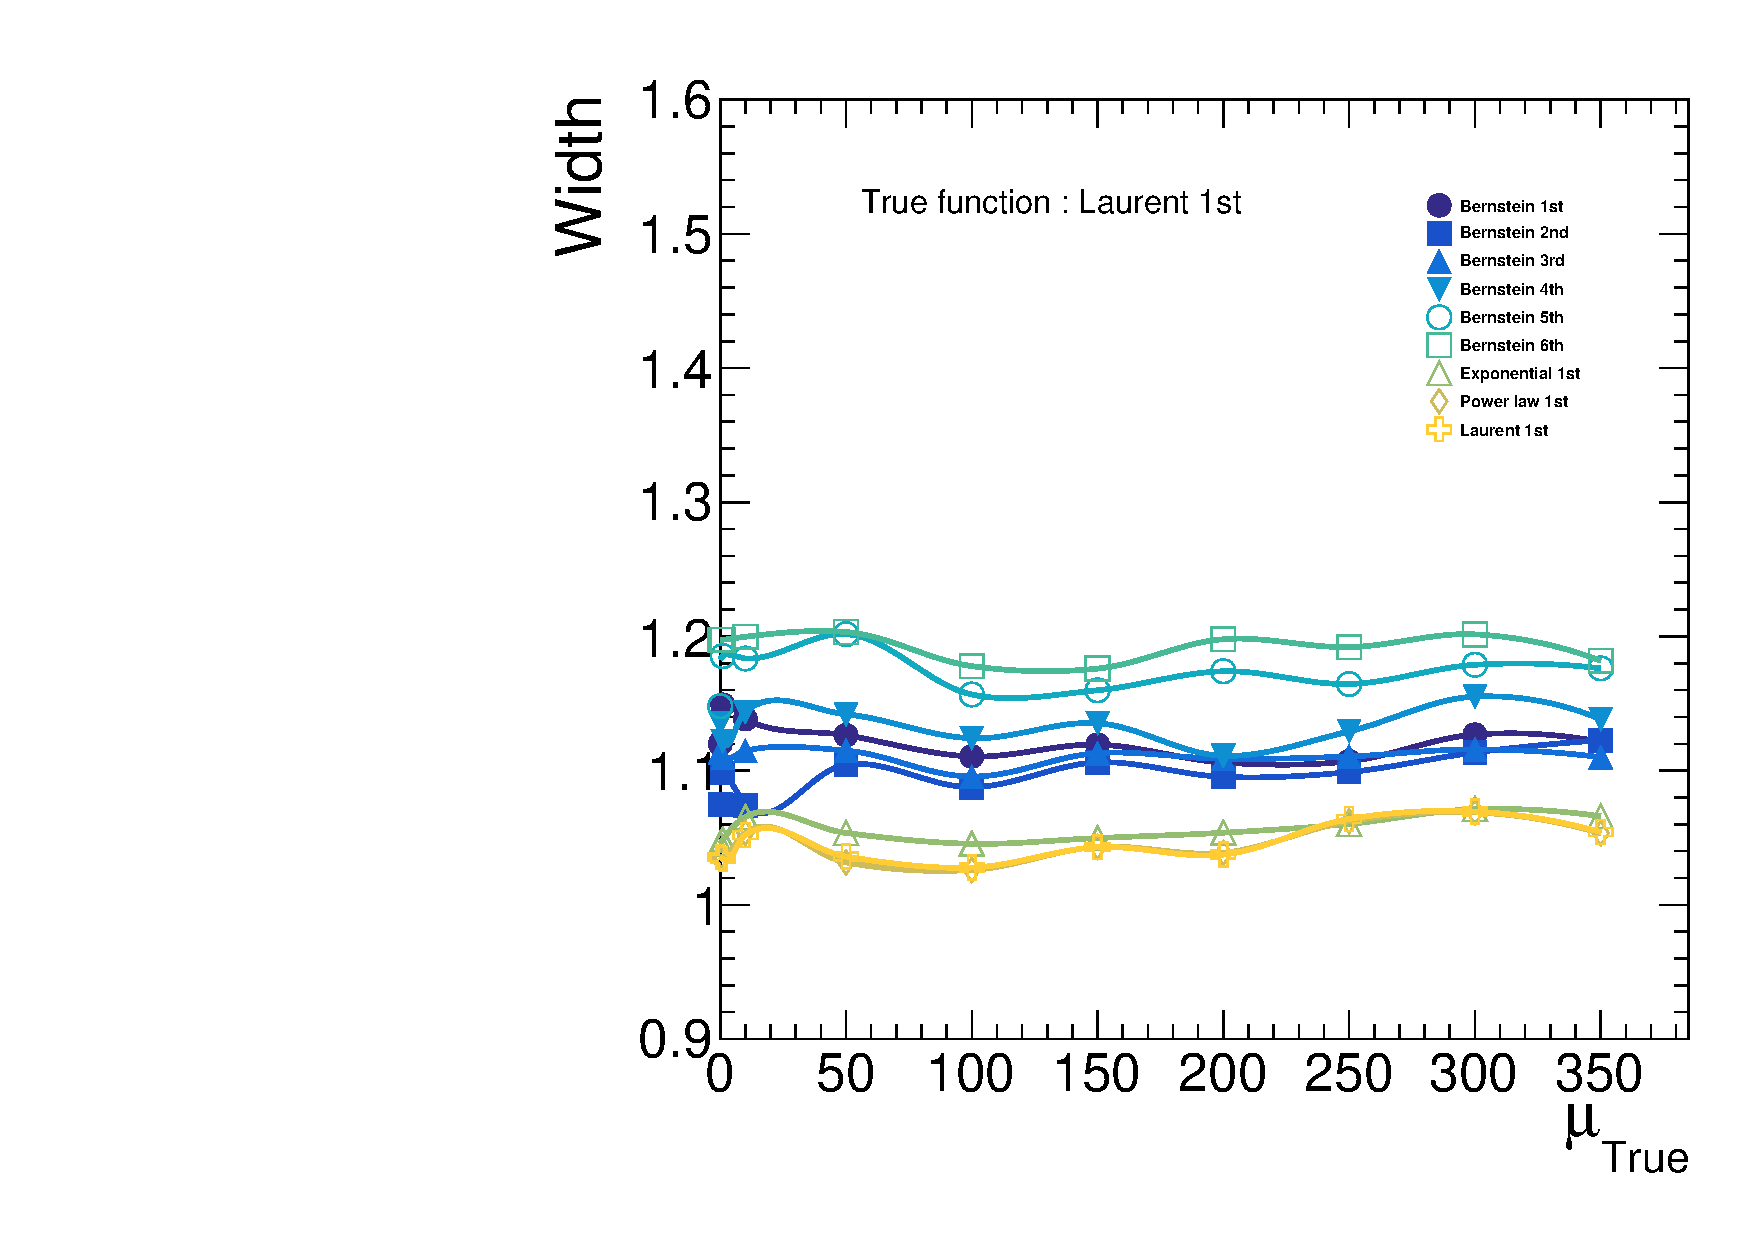
\includegraphics[width=0.33\textwidth]{Fig/BiasStudy/Linearity/HJpsiG/pull_width_linearity_TrueFunc8}\\
  \caption{The evolution of the width of the pull value distribution as more signal events are introduced in the Higgs decay.}
  \label{fig:Linearity_width_HJpsiG}
\end{figure}
\clearpage
%
\subsection{$Z\to \JPsi\ \gamma$ Cat1}
\begin{figure}[!ht]
  \centering
  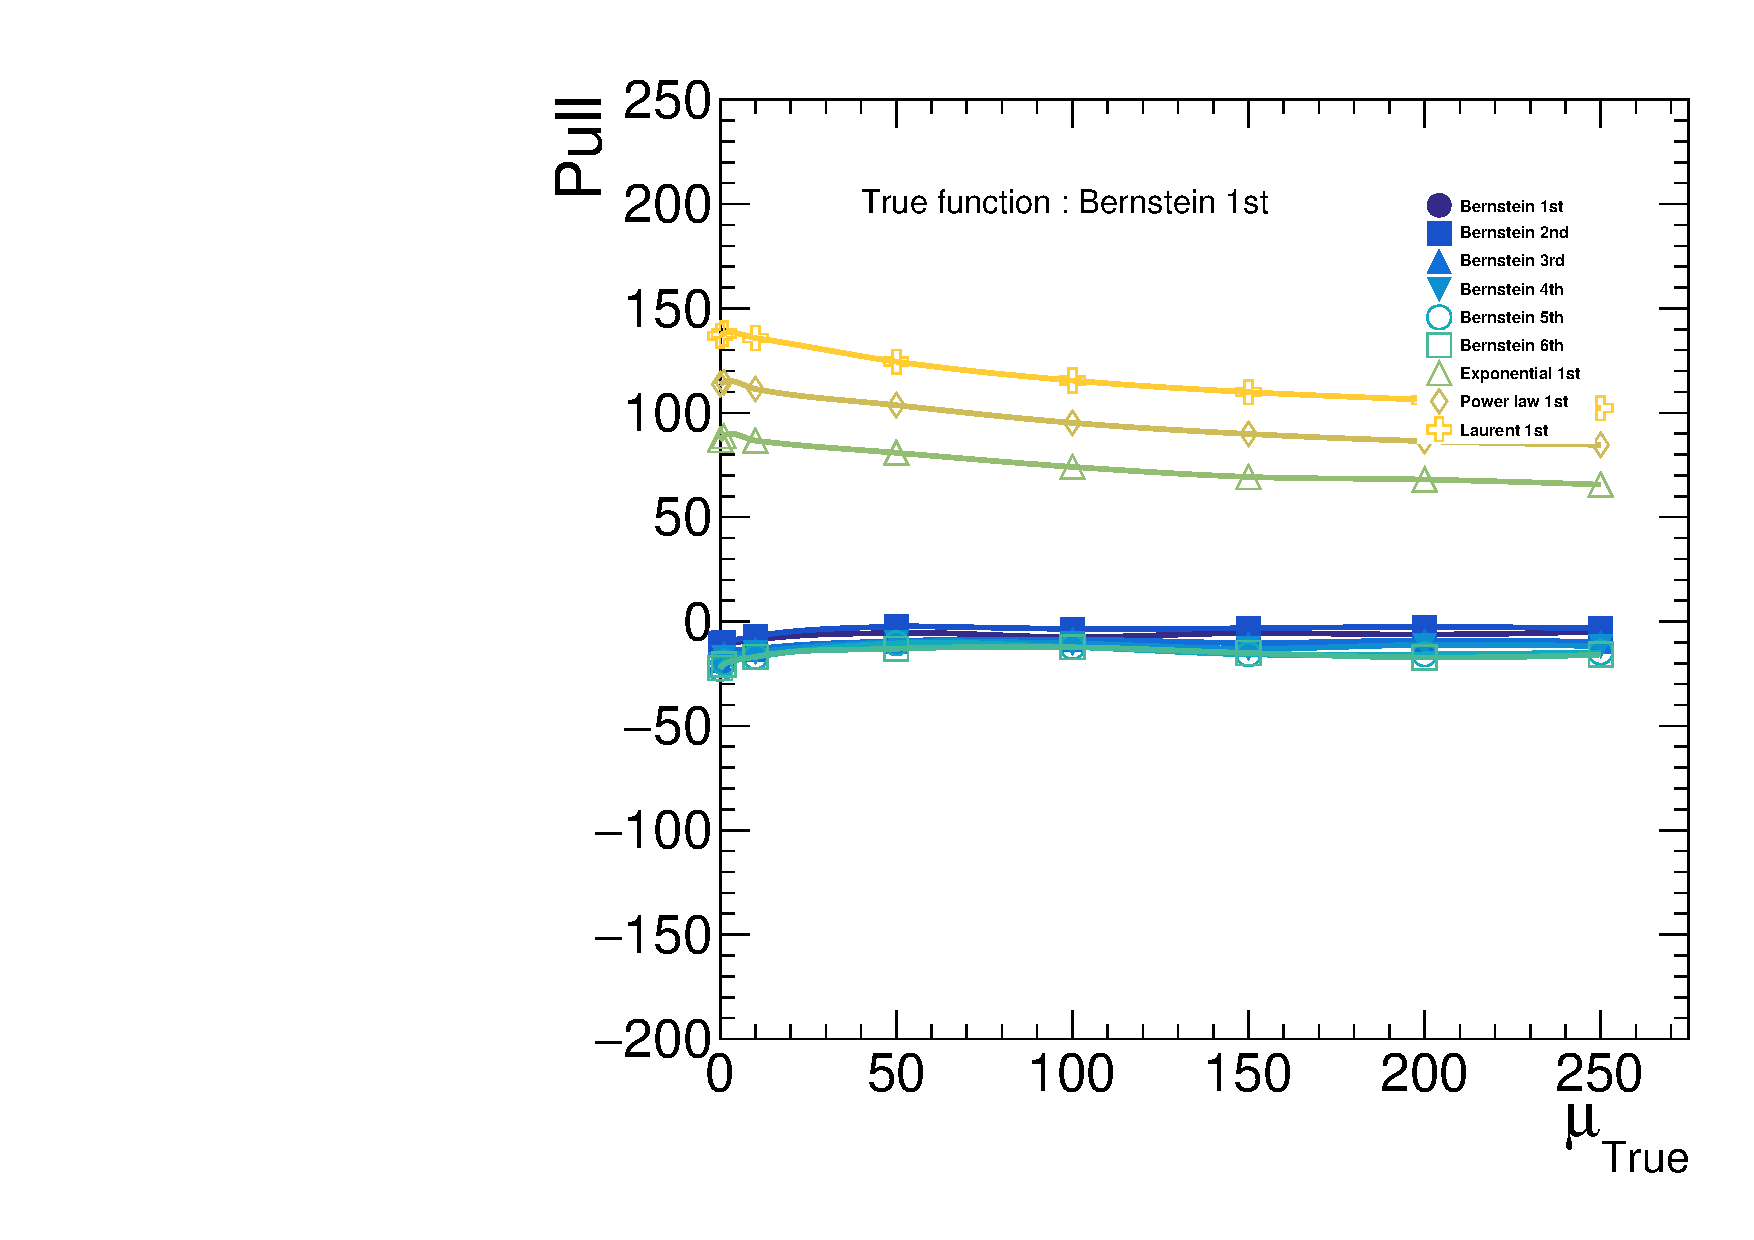
\includegraphics[width=0.33\textwidth]{Fig/BiasStudy/Linearity/ZJpsiG_Cat1/pull_mean_linearity_TrueFunc0}~
  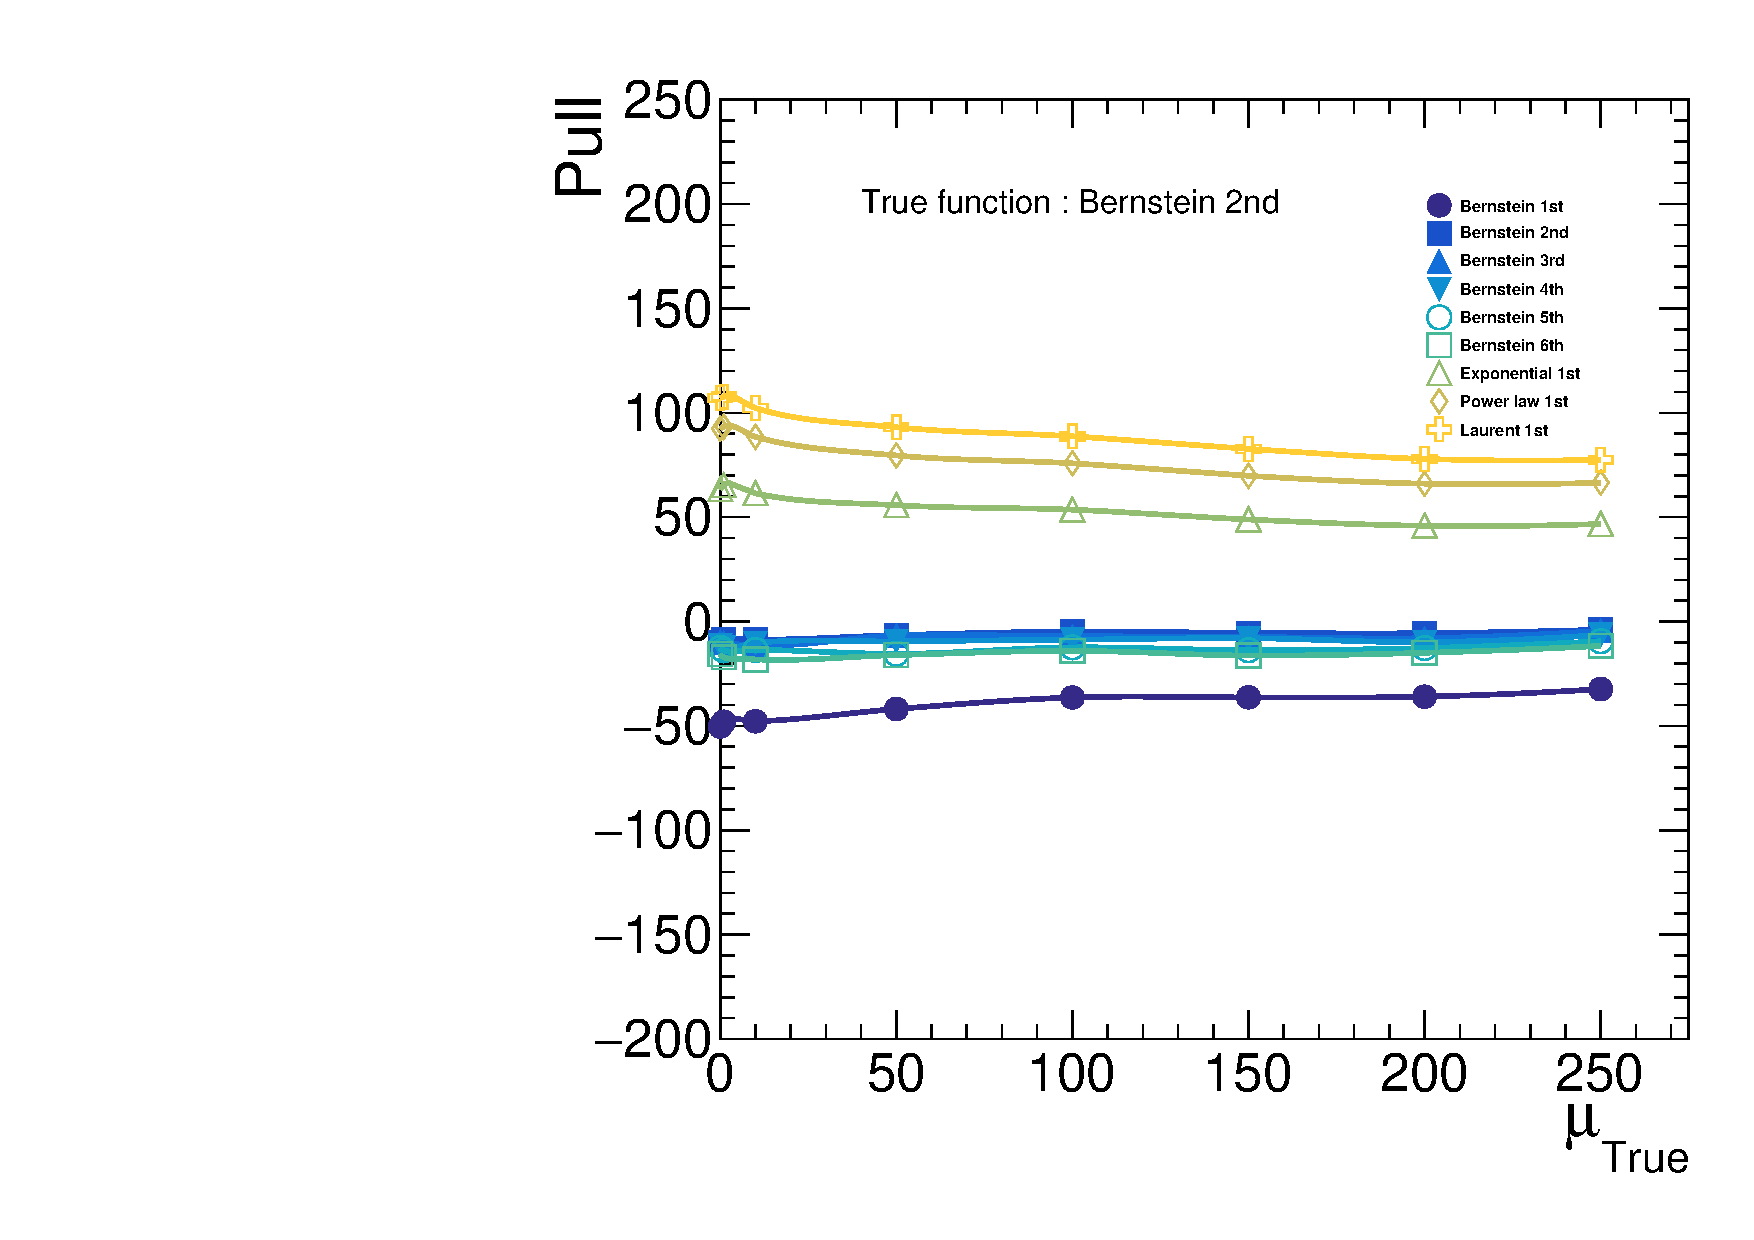
\includegraphics[width=0.33\textwidth]{Fig/BiasStudy/Linearity/ZJpsiG_Cat1/pull_mean_linearity_TrueFunc1}~
  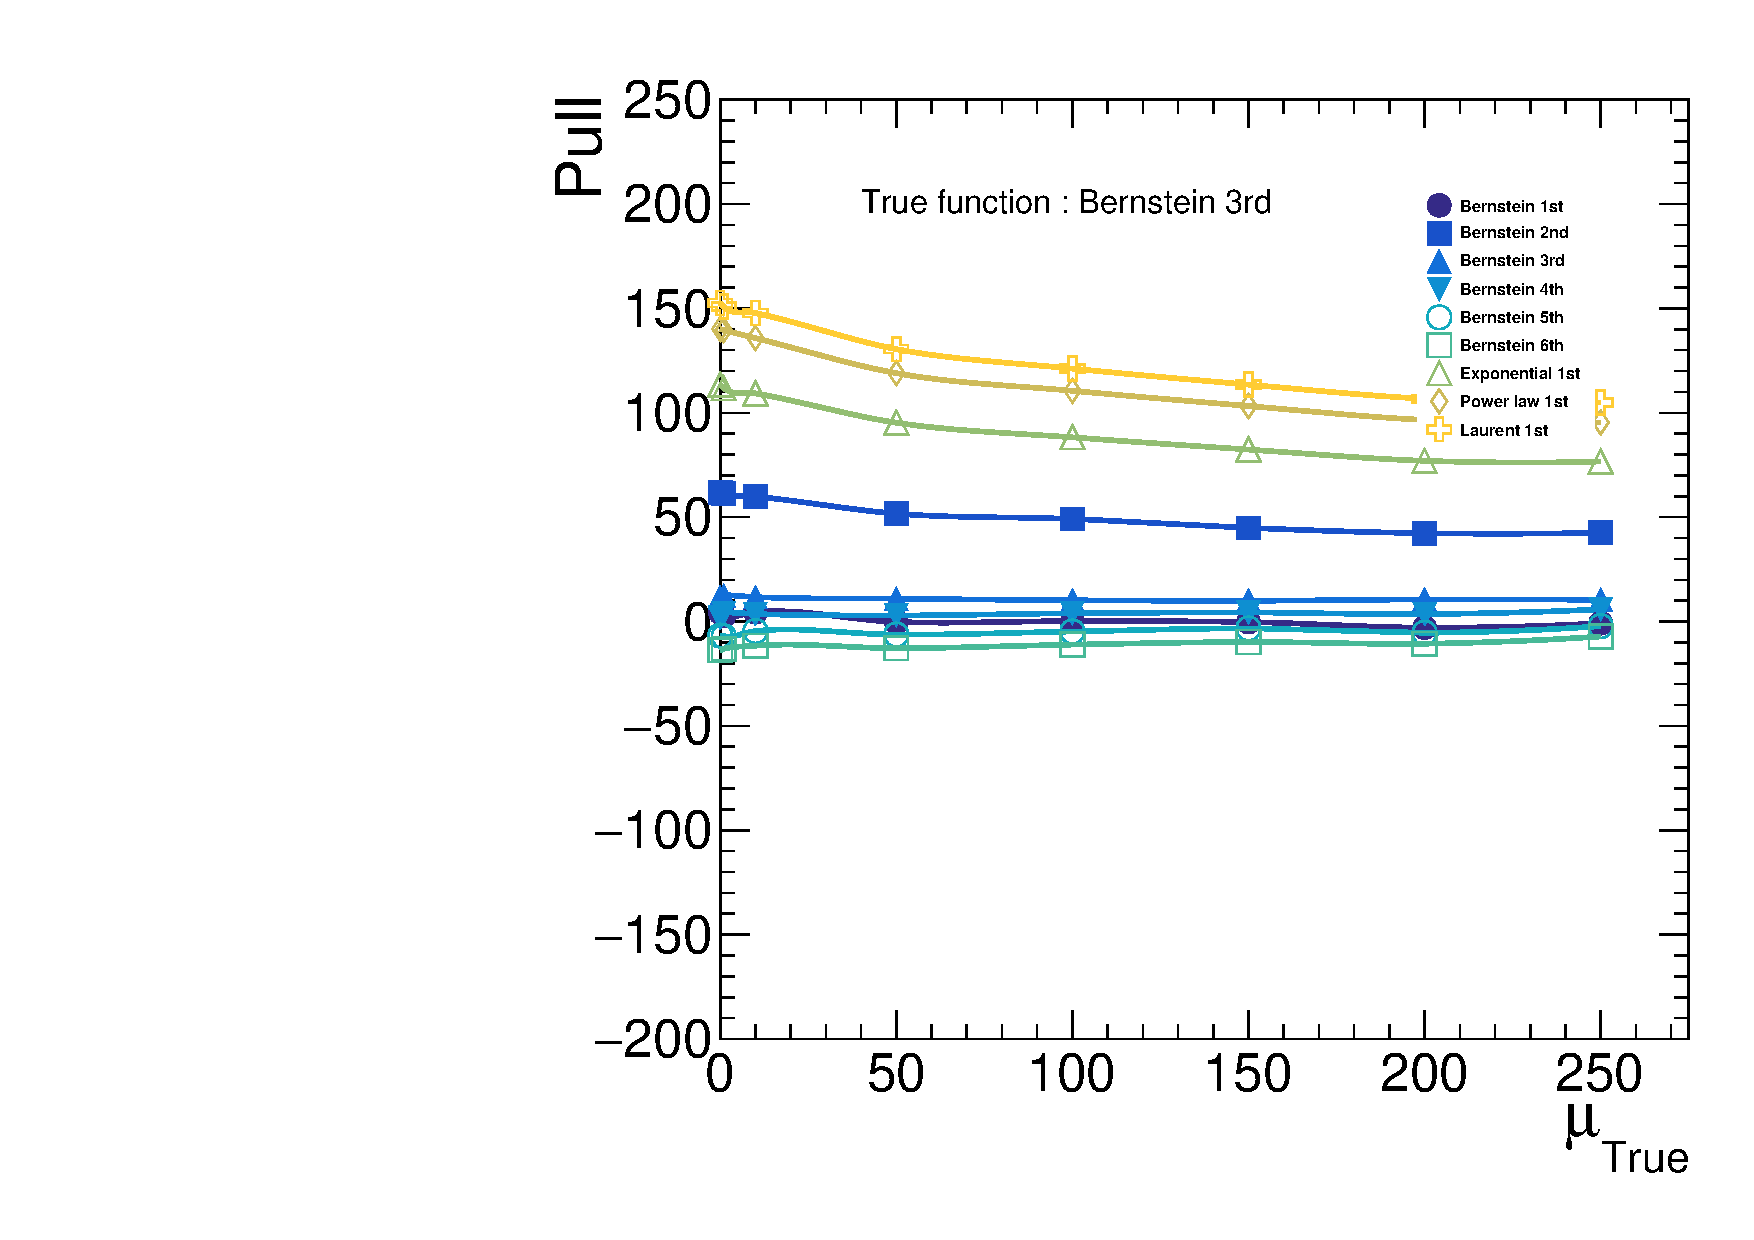
\includegraphics[width=0.33\textwidth]{Fig/BiasStudy/Linearity/ZJpsiG_Cat1/pull_mean_linearity_TrueFunc2}\\
  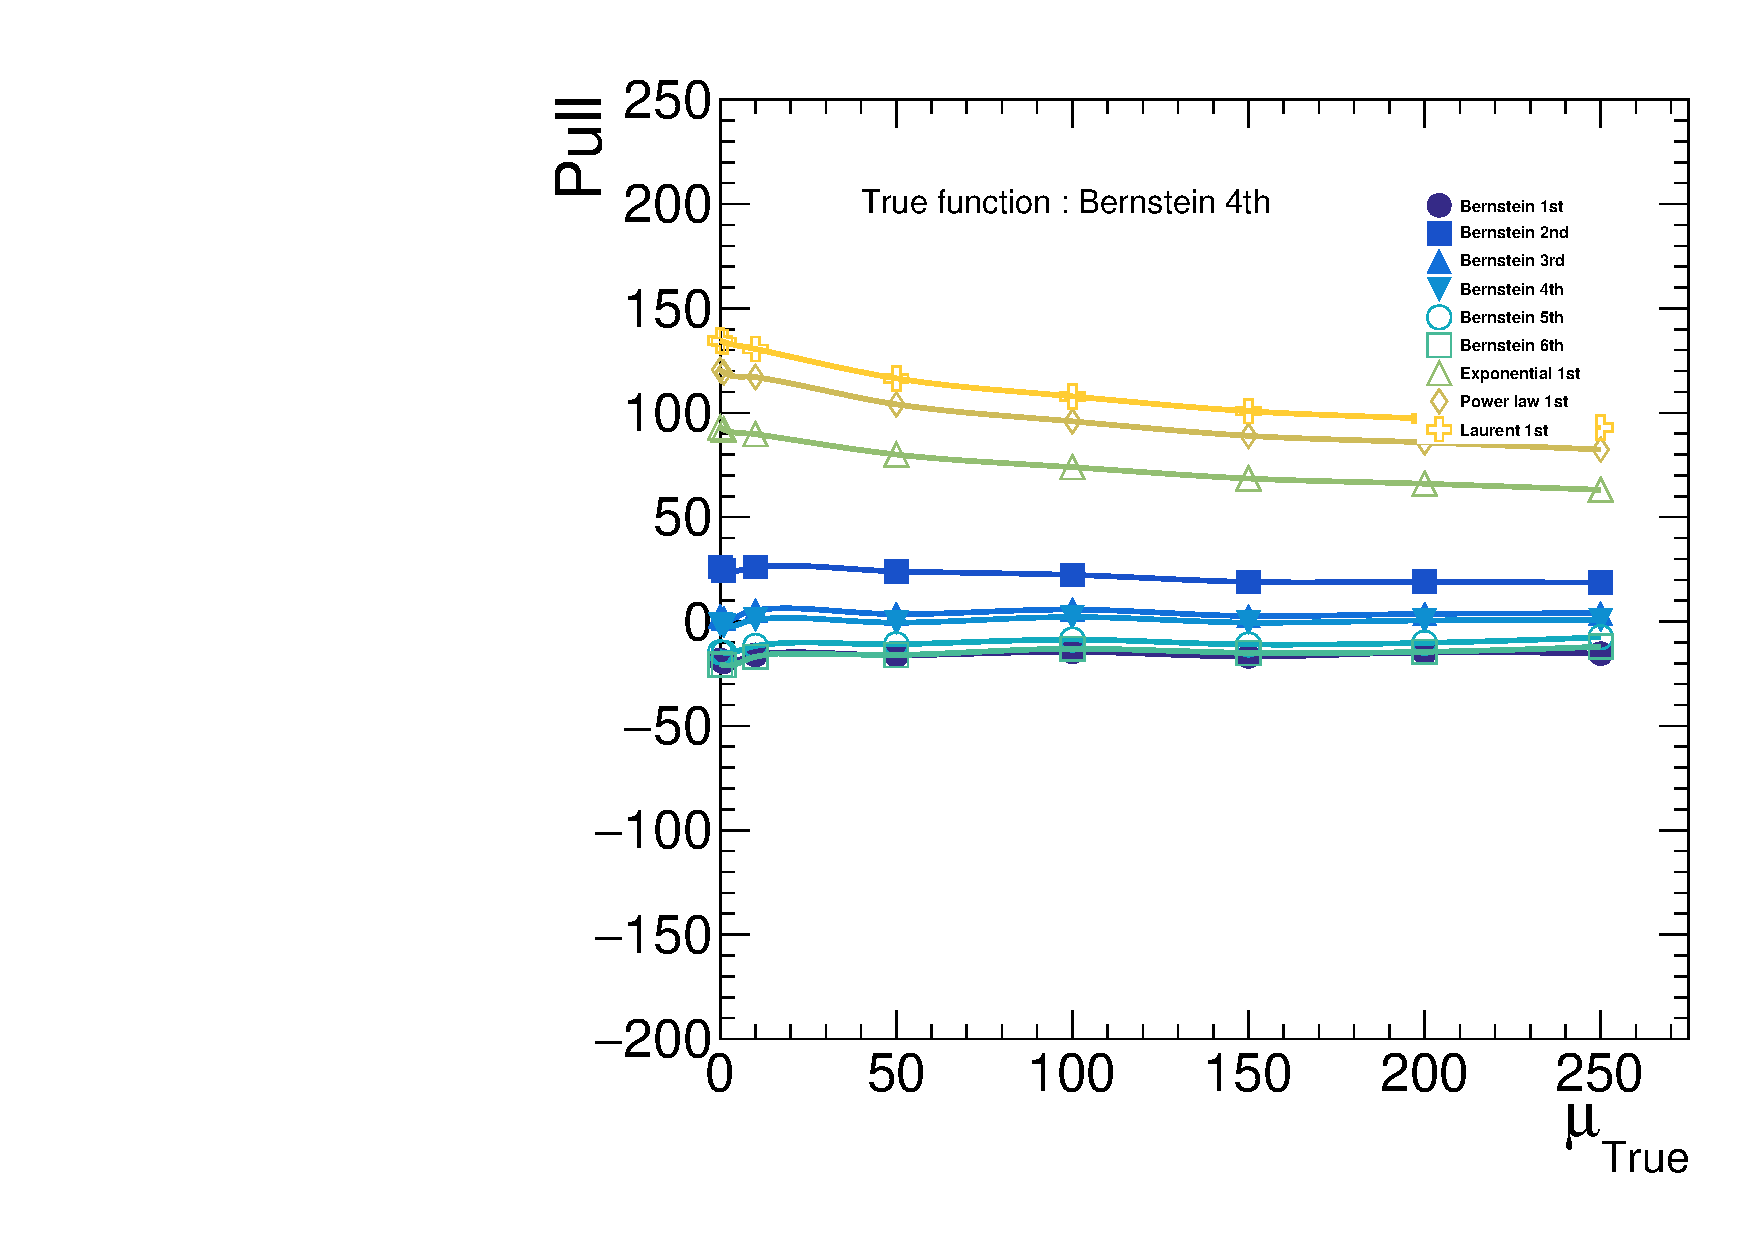
\includegraphics[width=0.33\textwidth]{Fig/BiasStudy/Linearity/ZJpsiG_Cat1/pull_mean_linearity_TrueFunc3}~
  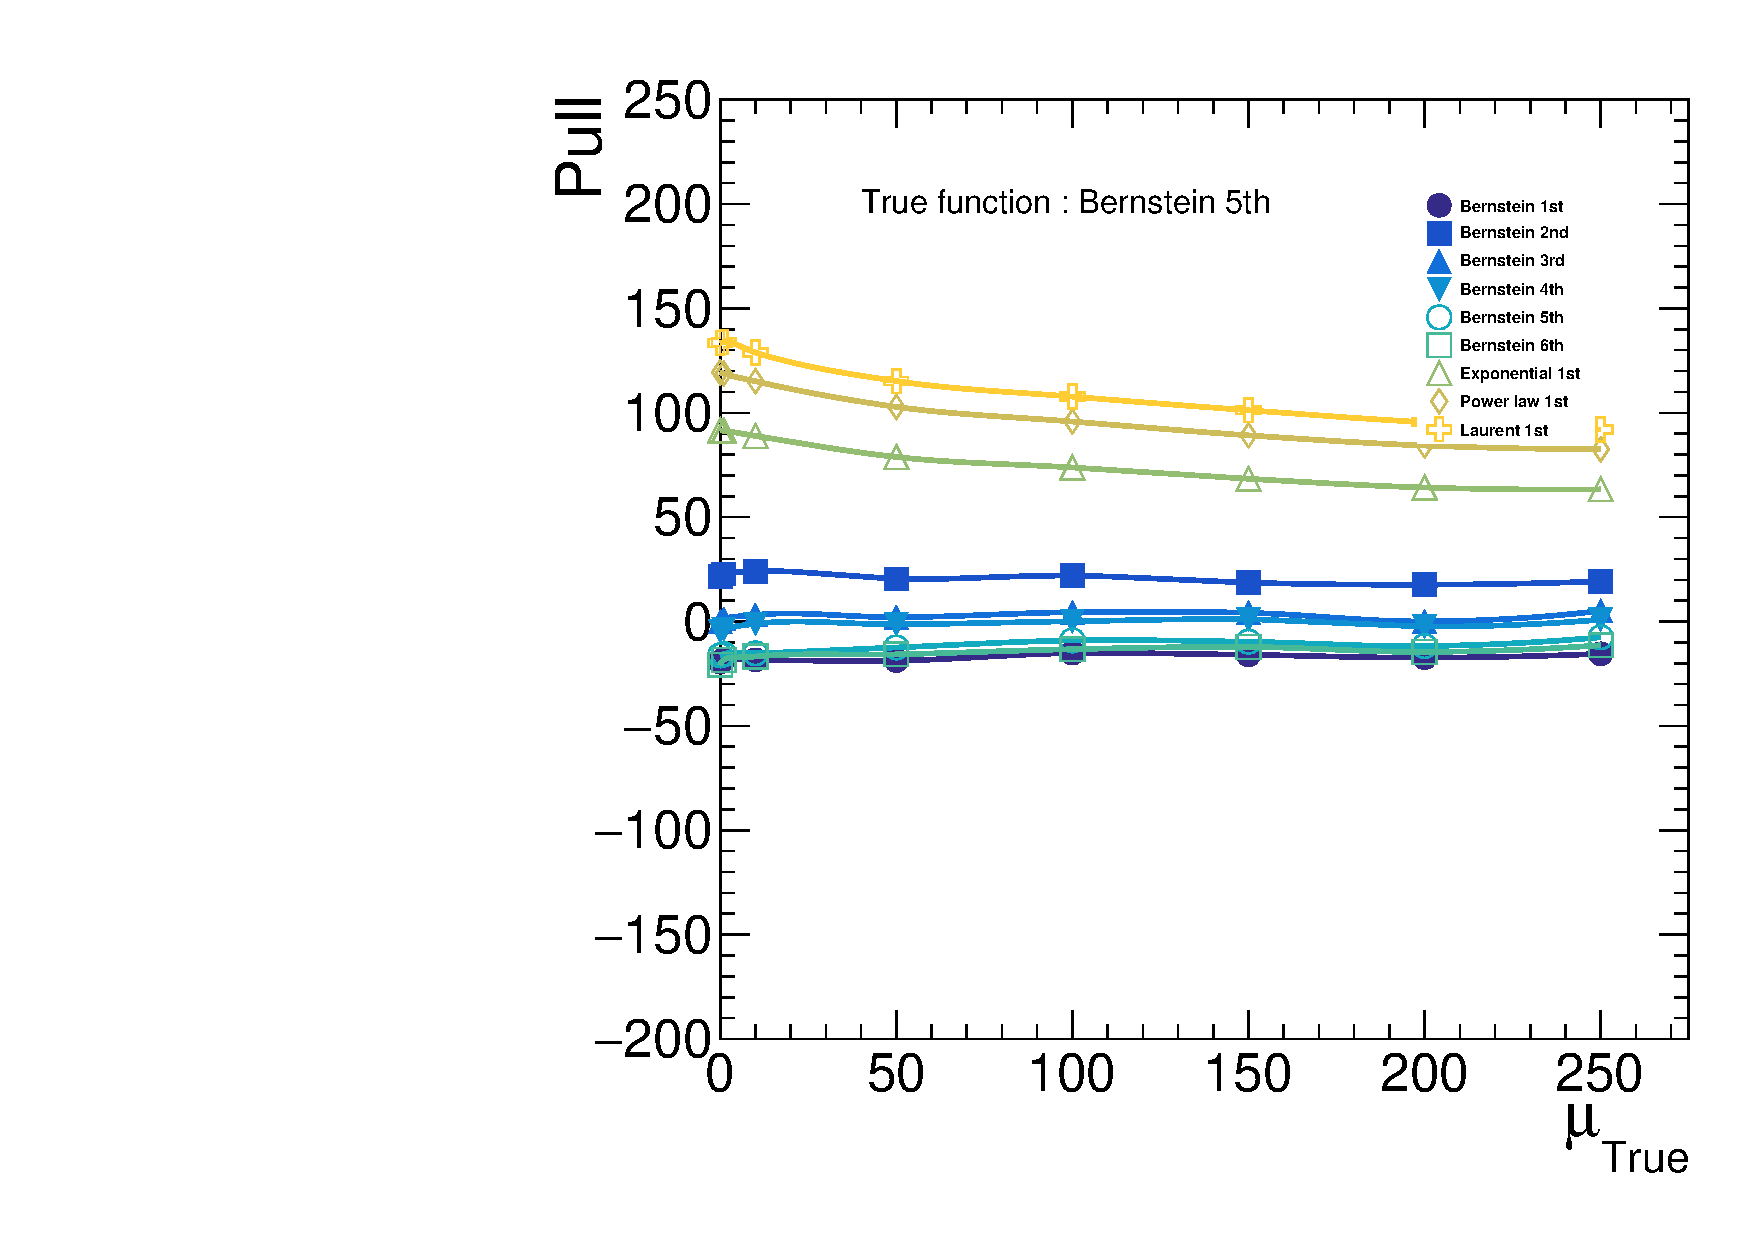
\includegraphics[width=0.33\textwidth]{Fig/BiasStudy/Linearity/ZJpsiG_Cat1/pull_mean_linearity_TrueFunc4}~
  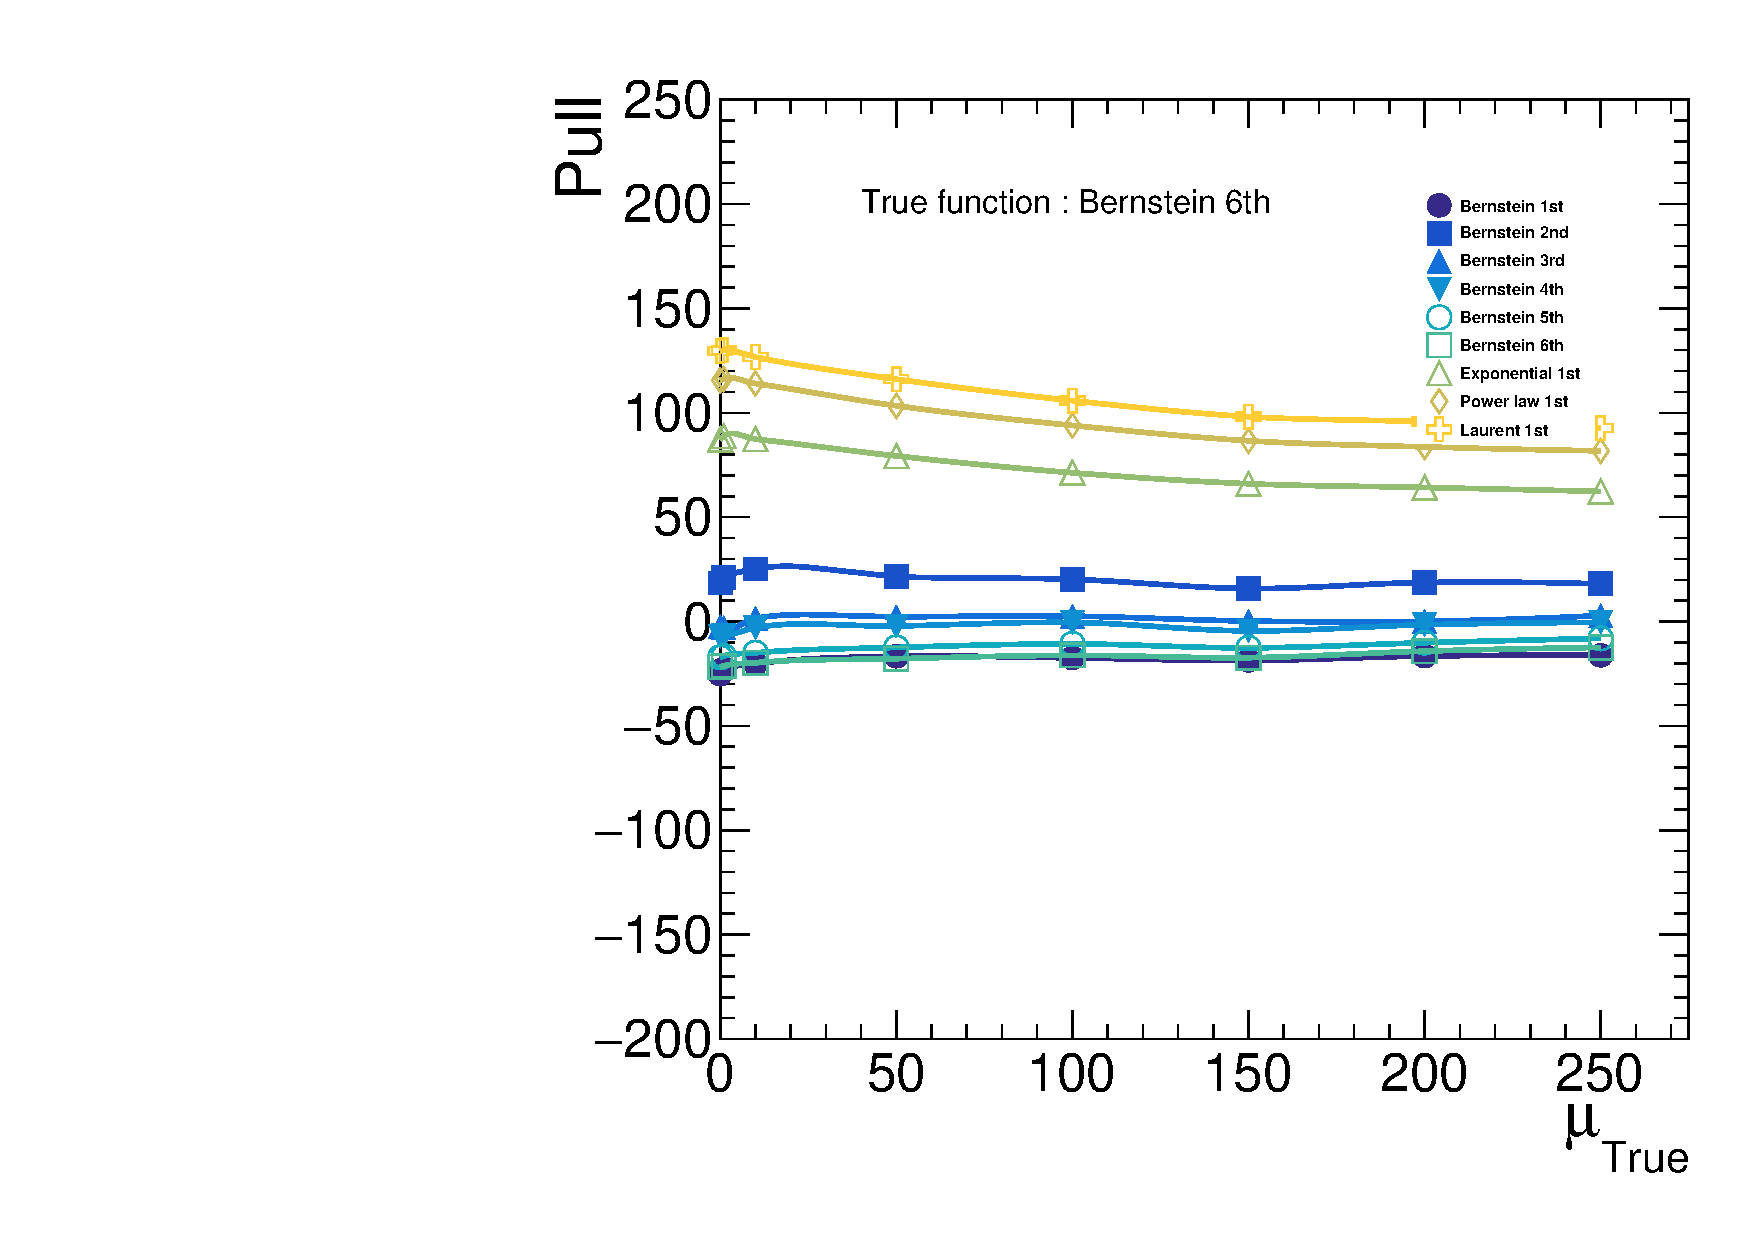
\includegraphics[width=0.33\textwidth]{Fig/BiasStudy/Linearity/ZJpsiG_Cat1/pull_mean_linearity_TrueFunc5}\\
  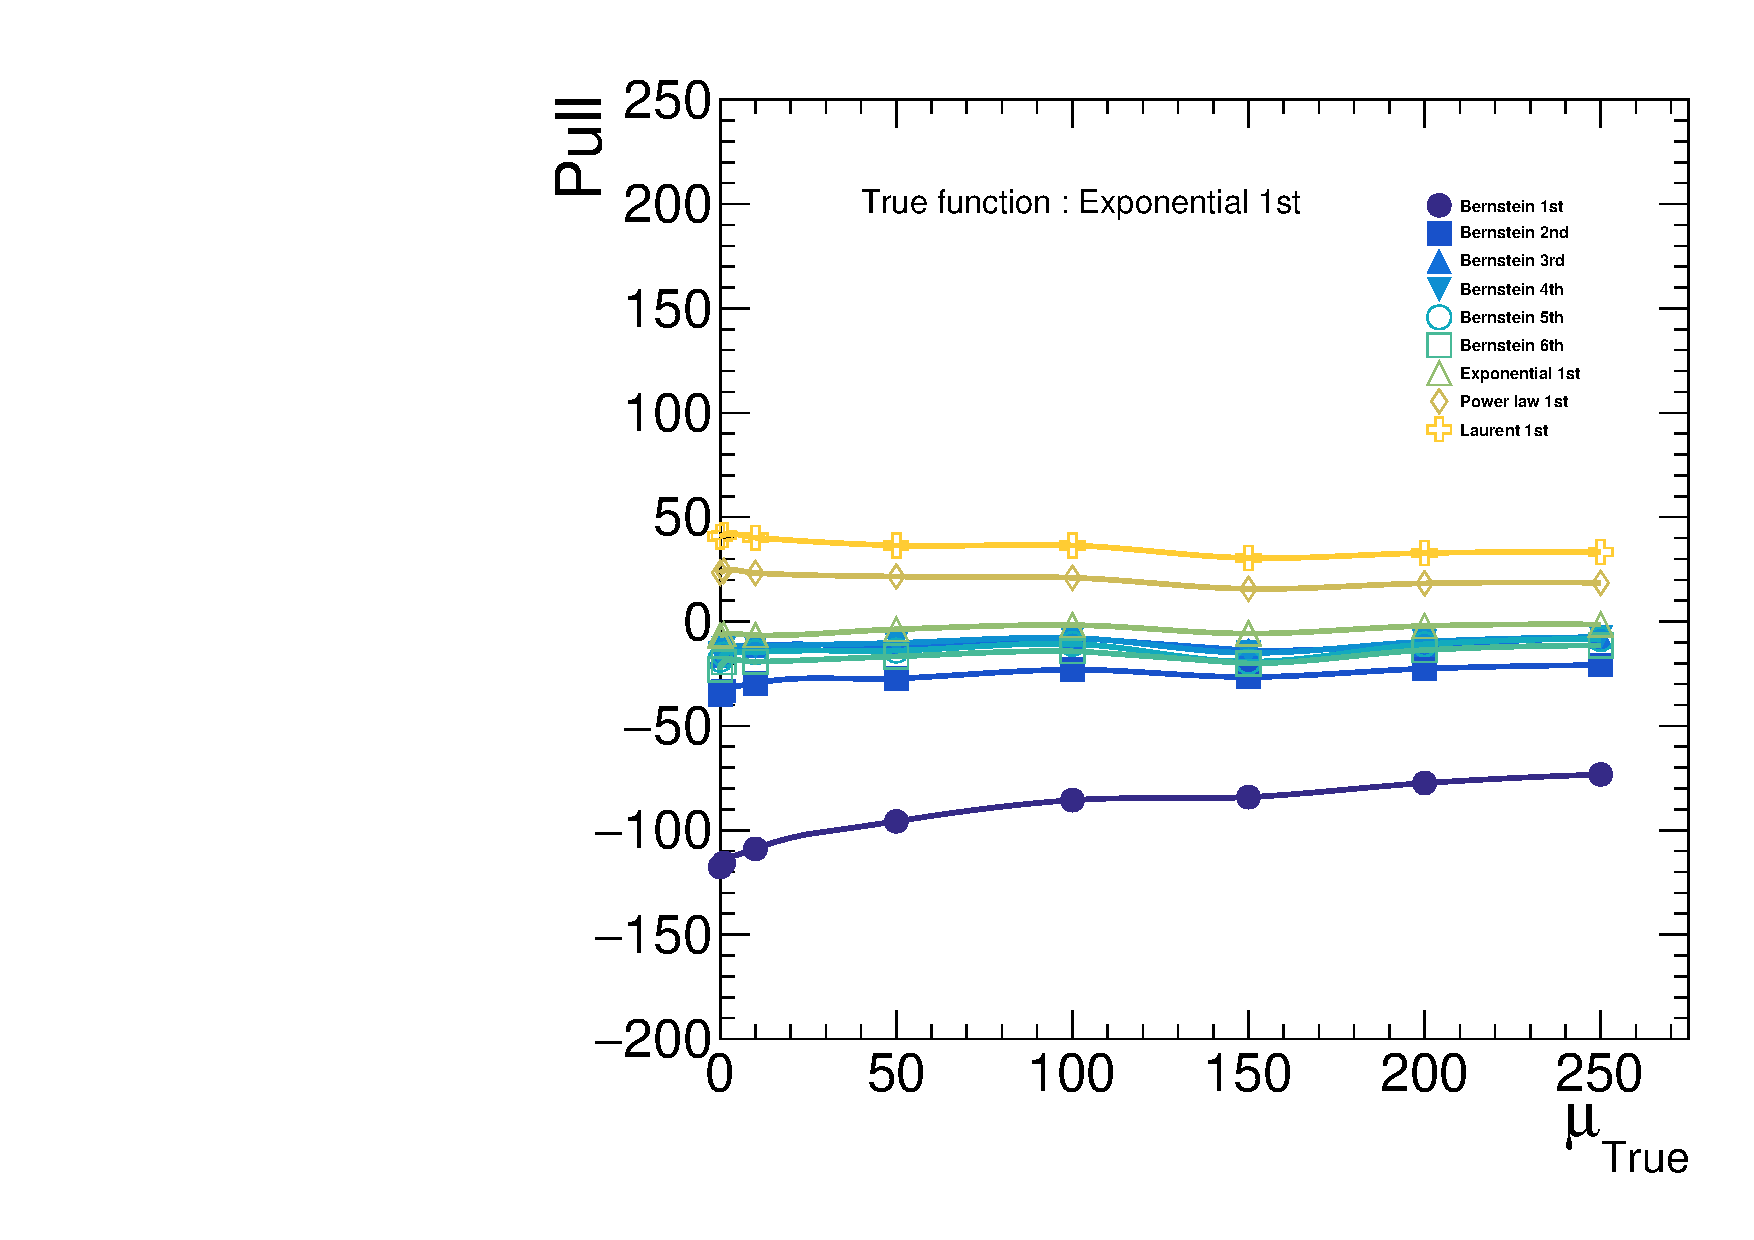
\includegraphics[width=0.33\textwidth]{Fig/BiasStudy/Linearity/ZJpsiG_Cat1/pull_mean_linearity_TrueFunc6}~
  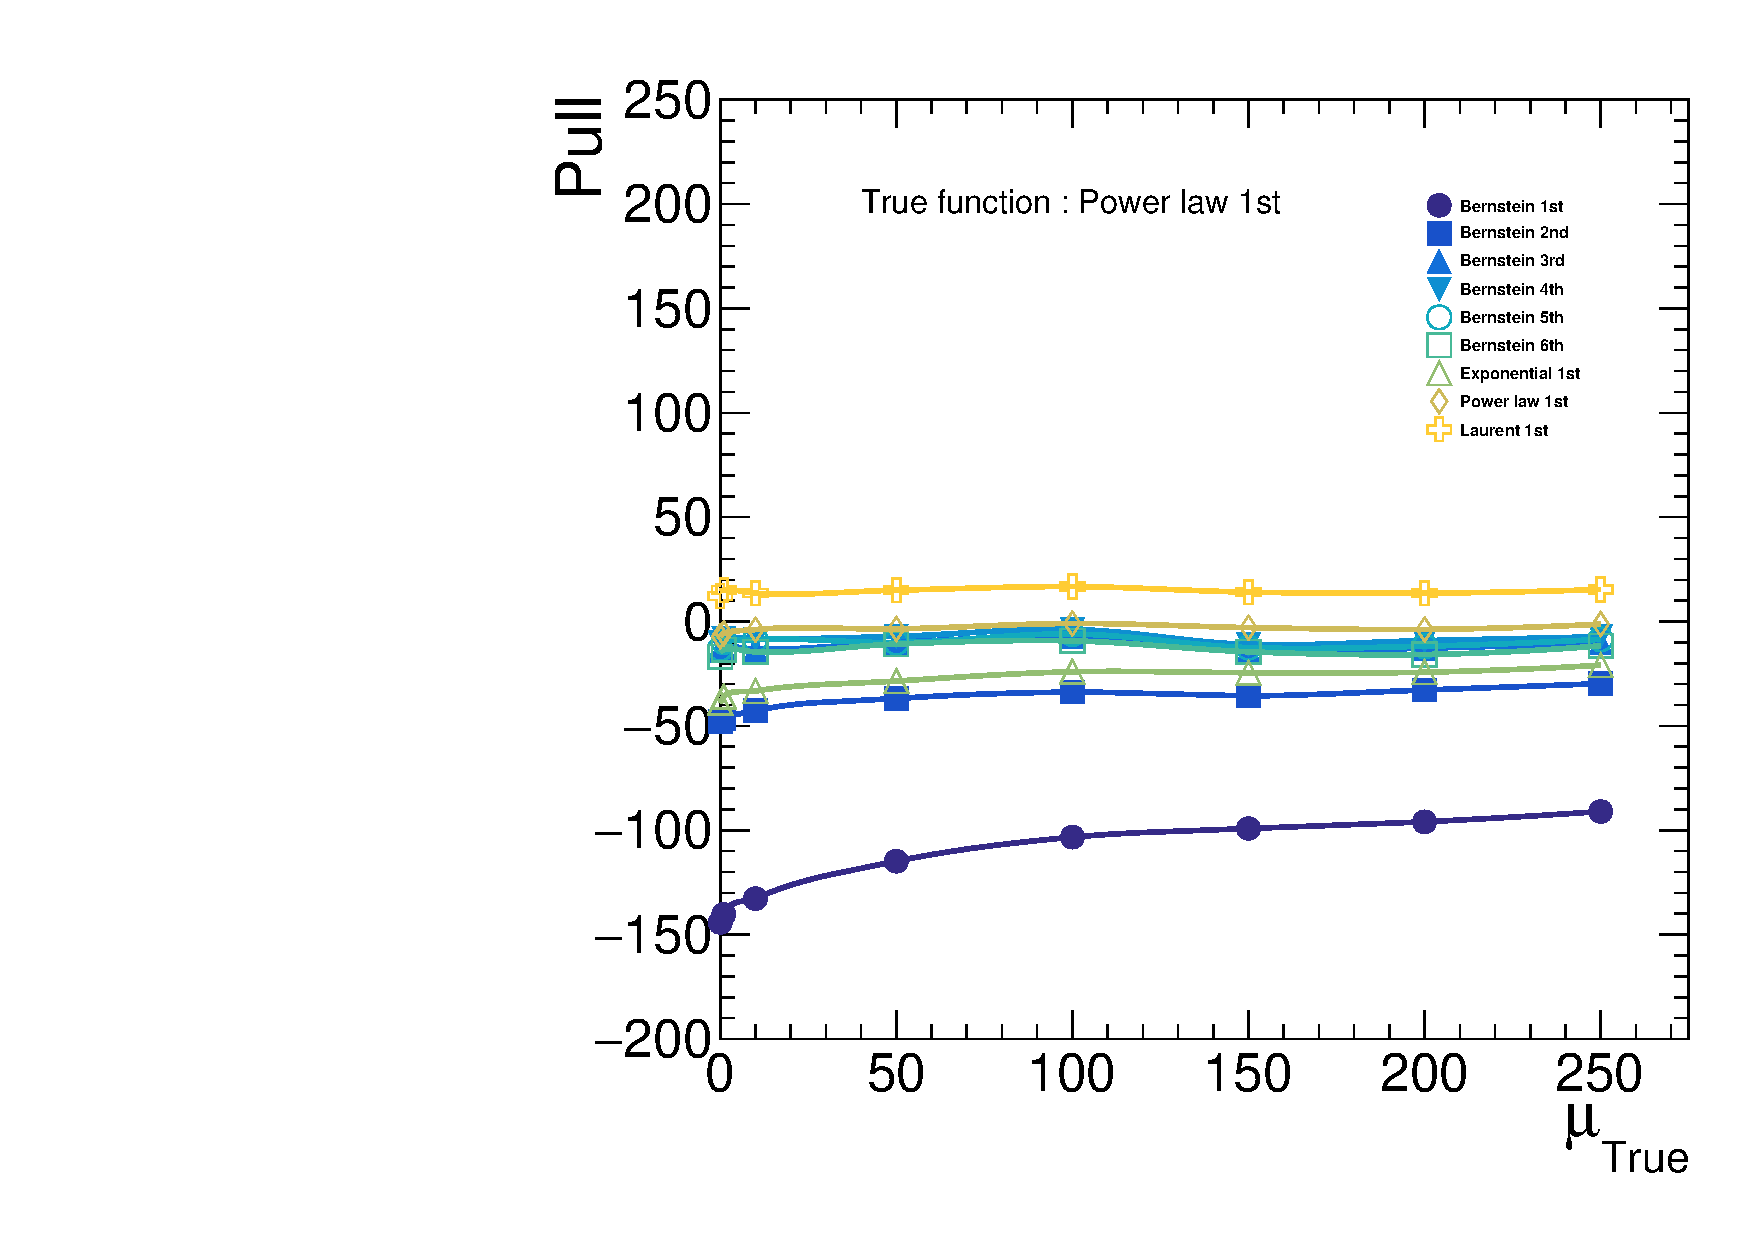
\includegraphics[width=0.33\textwidth]{Fig/BiasStudy/Linearity/ZJpsiG_Cat1/pull_mean_linearity_TrueFunc7}~
  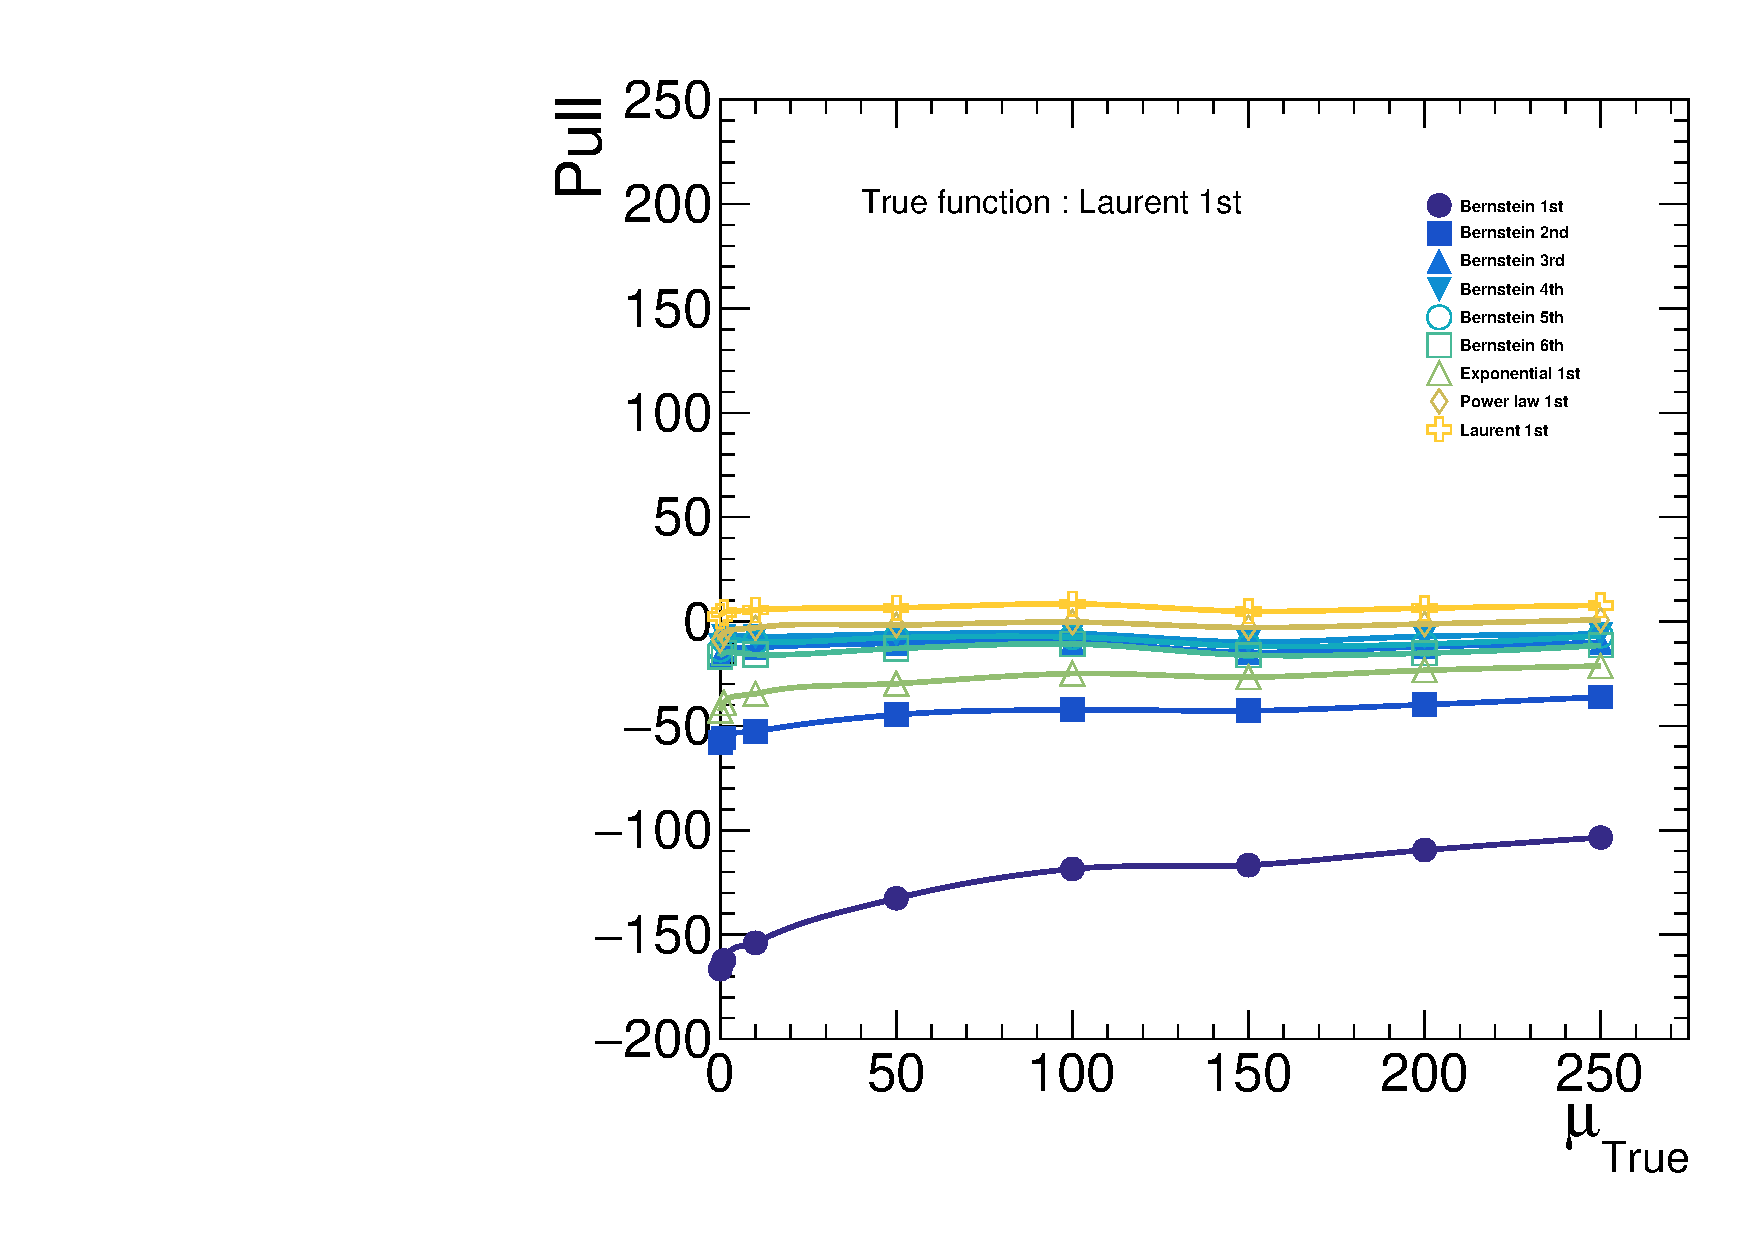
\includegraphics[width=0.33\textwidth]{Fig/BiasStudy/Linearity/ZJpsiG_Cat1/pull_mean_linearity_TrueFunc8}\\
  \caption{The evolution of the mean of the pull value distribution as more signal events are introduced in the Cat1 of the Z decay.}
  \label{fig:Linearity_mean_ZJpsiG_Cat1}
\end{figure}
\clearpage
%
\begin{figure}[!ht]
  \centering
  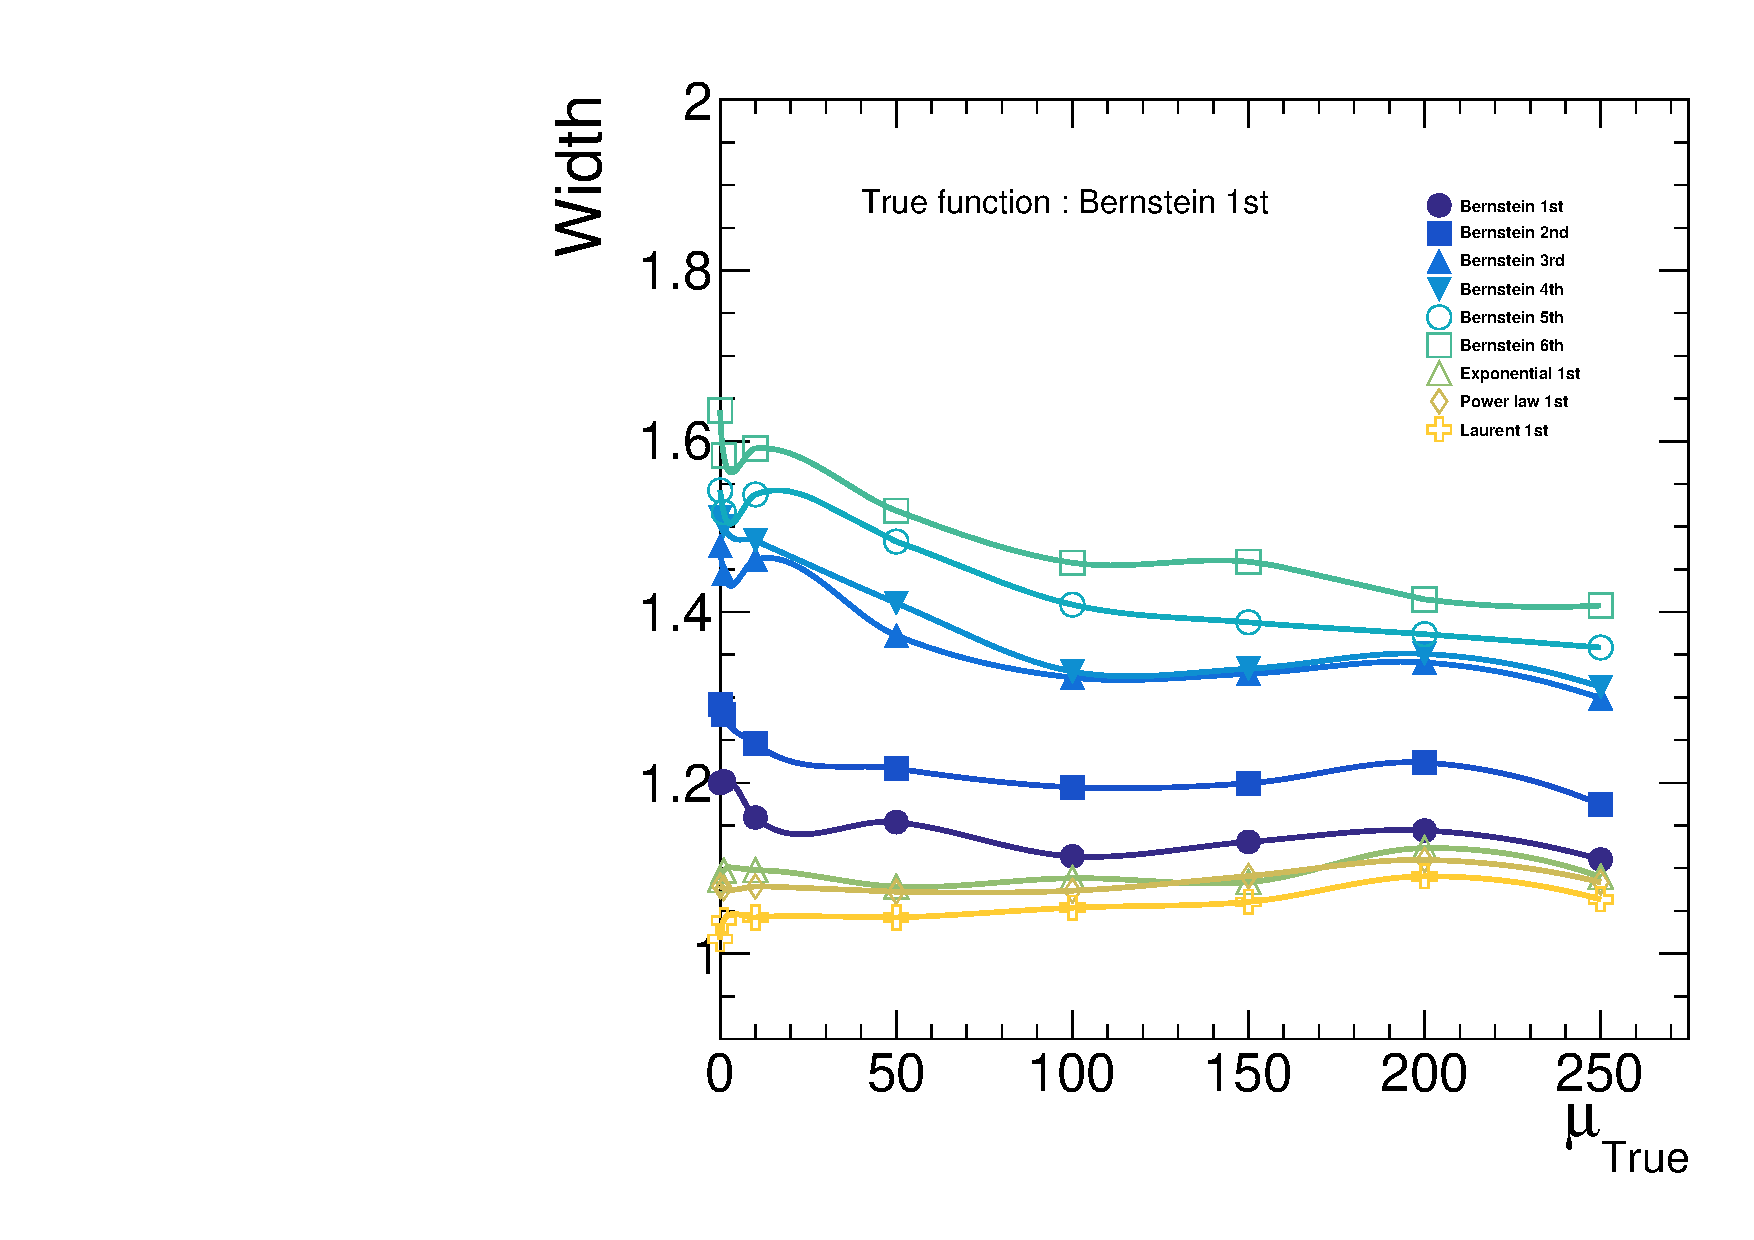
\includegraphics[width=0.33\textwidth]{Fig/BiasStudy/Linearity/ZJpsiG_Cat1/pull_width_linearity_TrueFunc0}~
  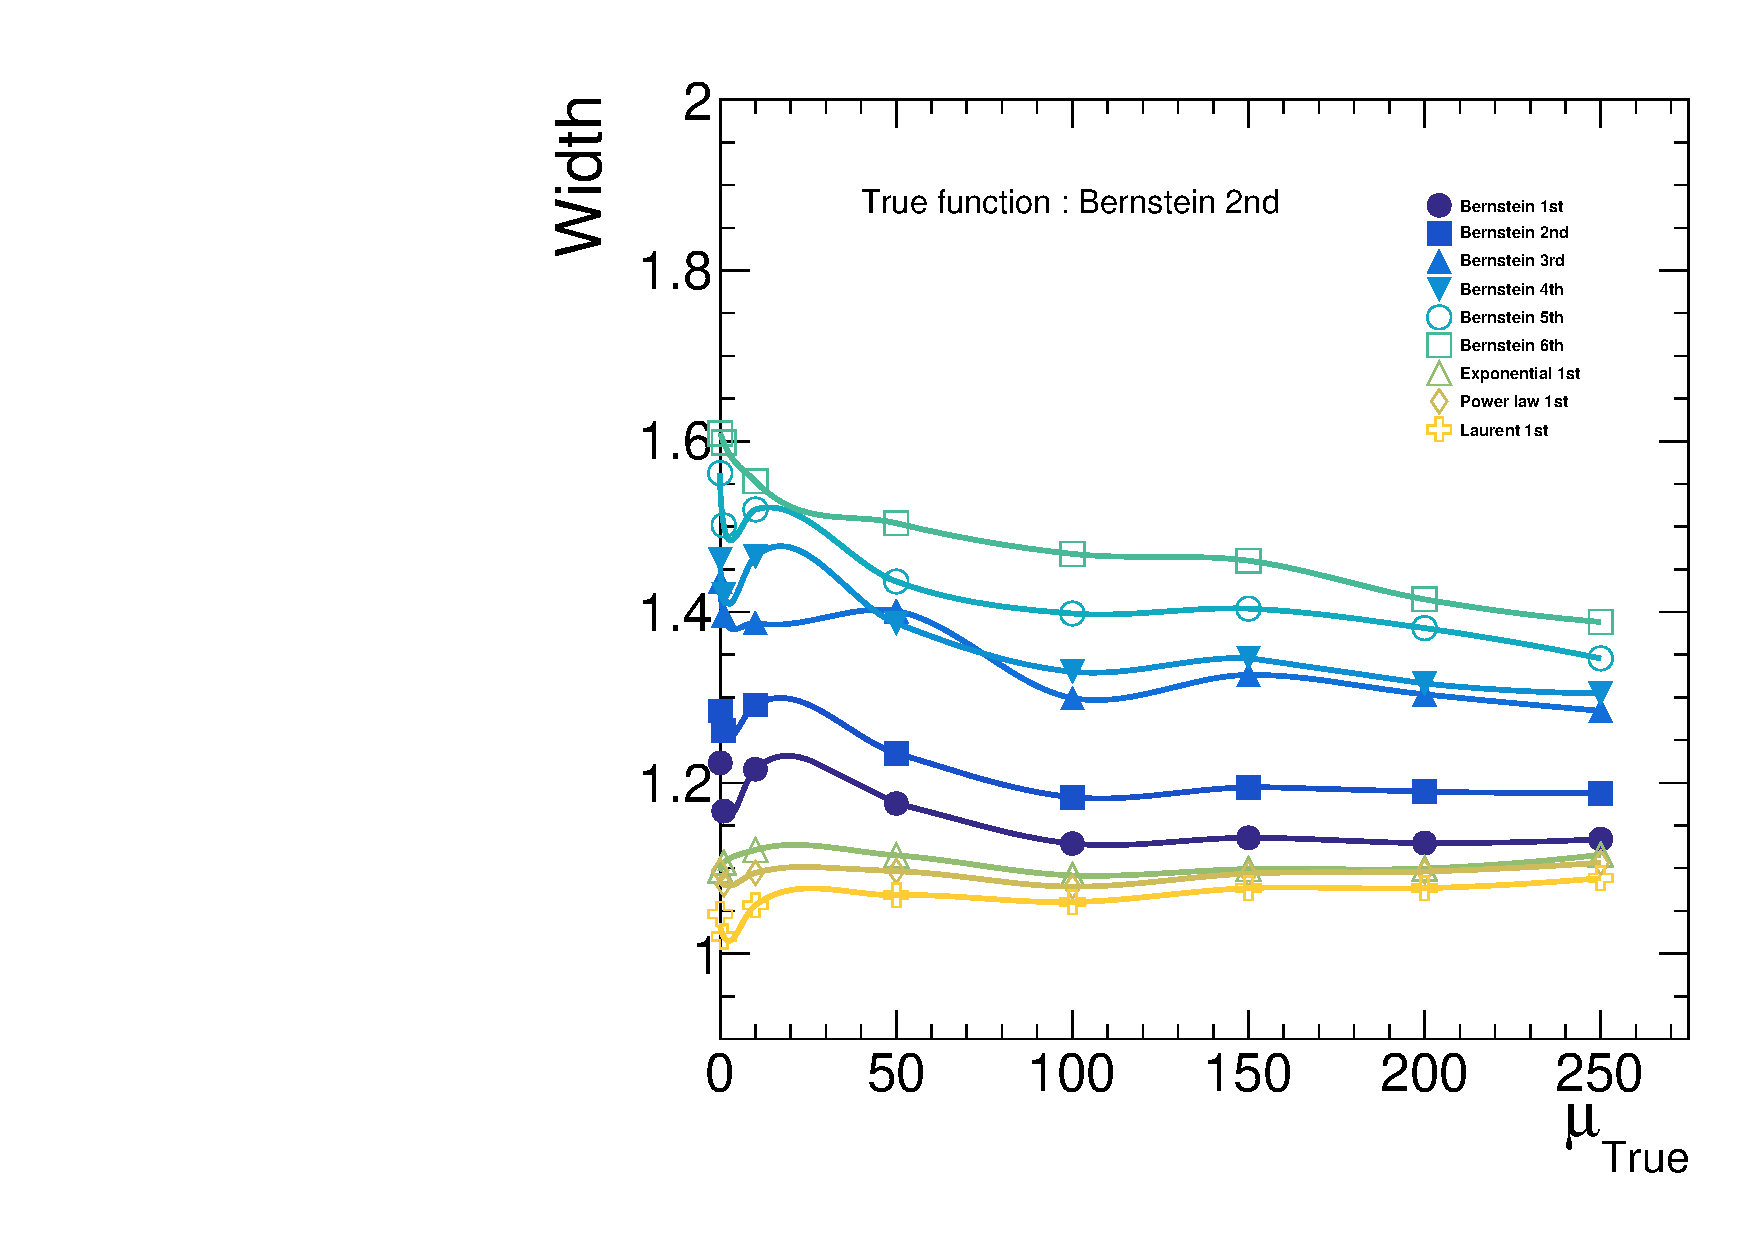
\includegraphics[width=0.33\textwidth]{Fig/BiasStudy/Linearity/ZJpsiG_Cat1/pull_width_linearity_TrueFunc1}~
  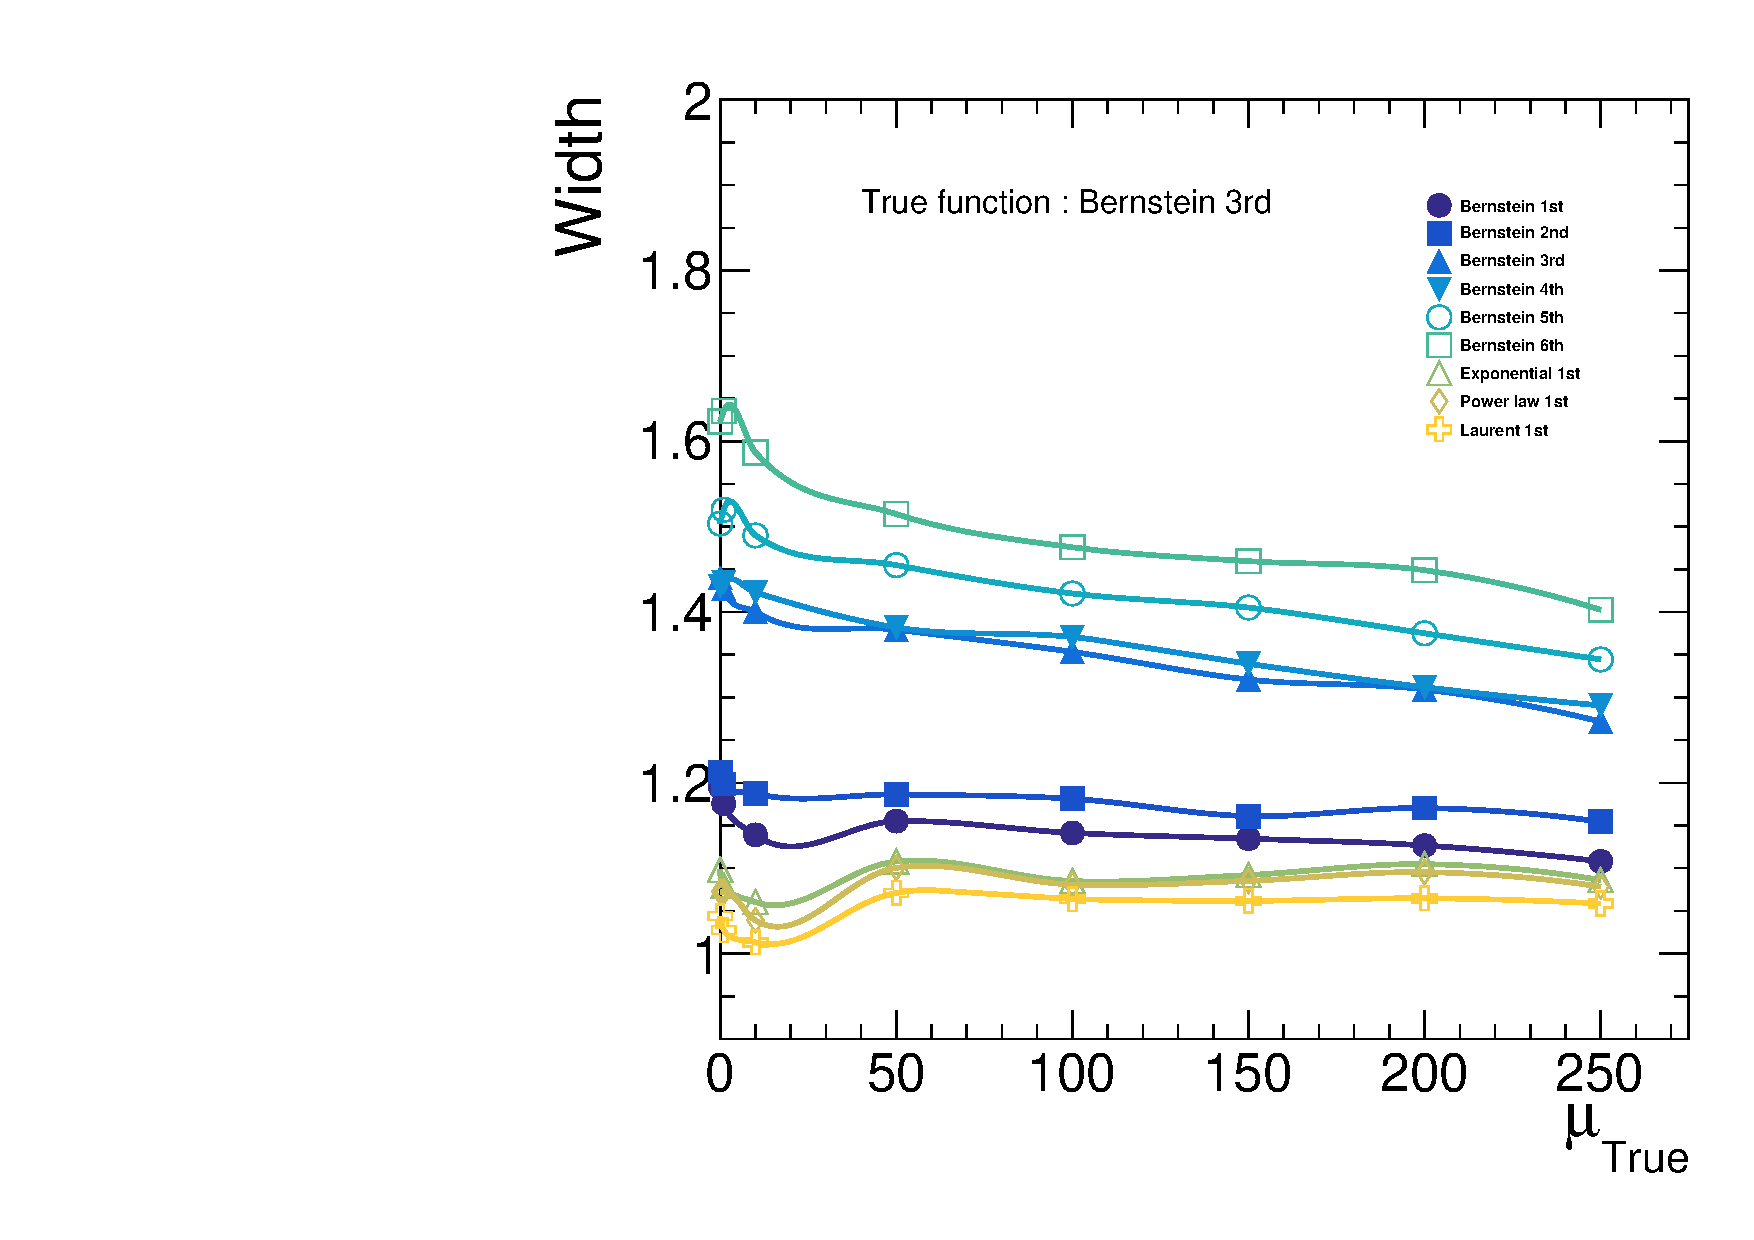
\includegraphics[width=0.33\textwidth]{Fig/BiasStudy/Linearity/ZJpsiG_Cat1/pull_width_linearity_TrueFunc2}\\
  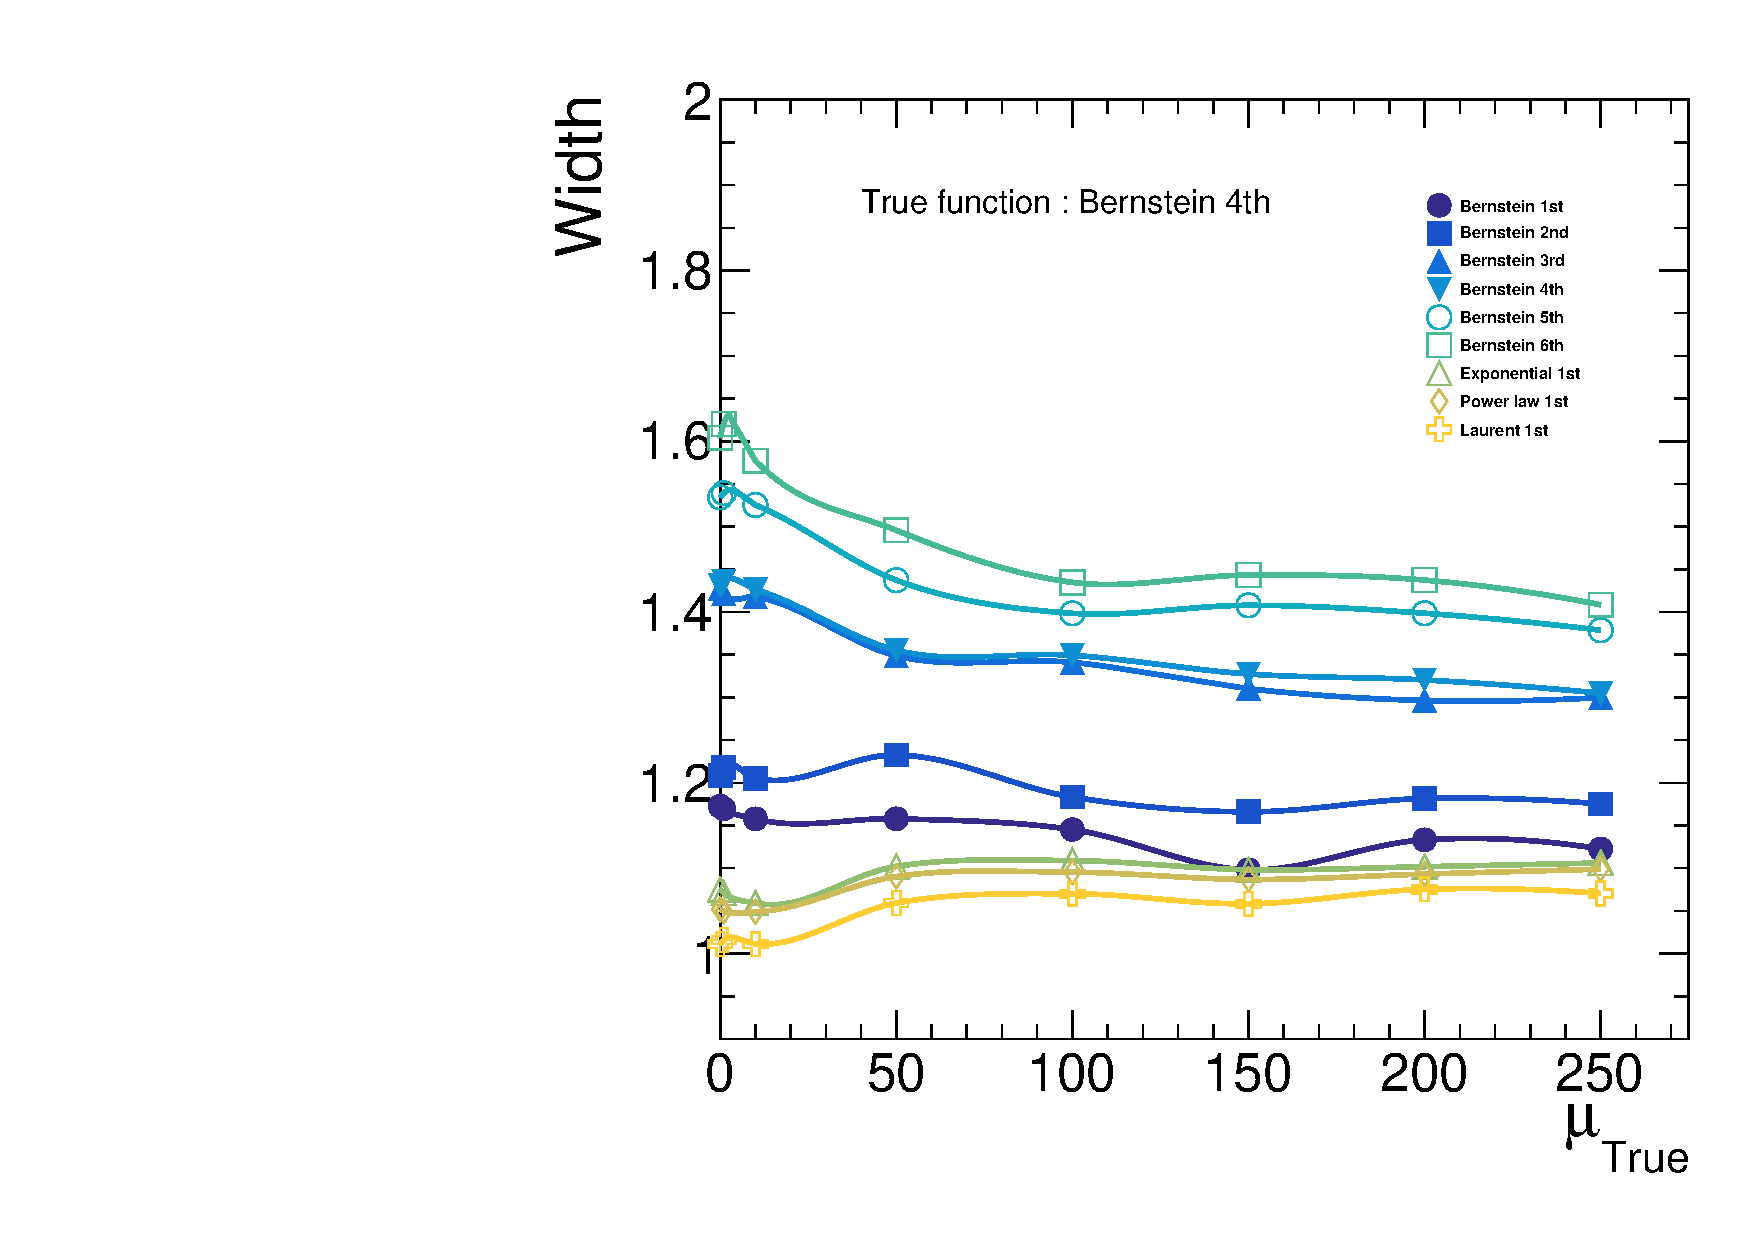
\includegraphics[width=0.33\textwidth]{Fig/BiasStudy/Linearity/ZJpsiG_Cat1/pull_width_linearity_TrueFunc3}~
  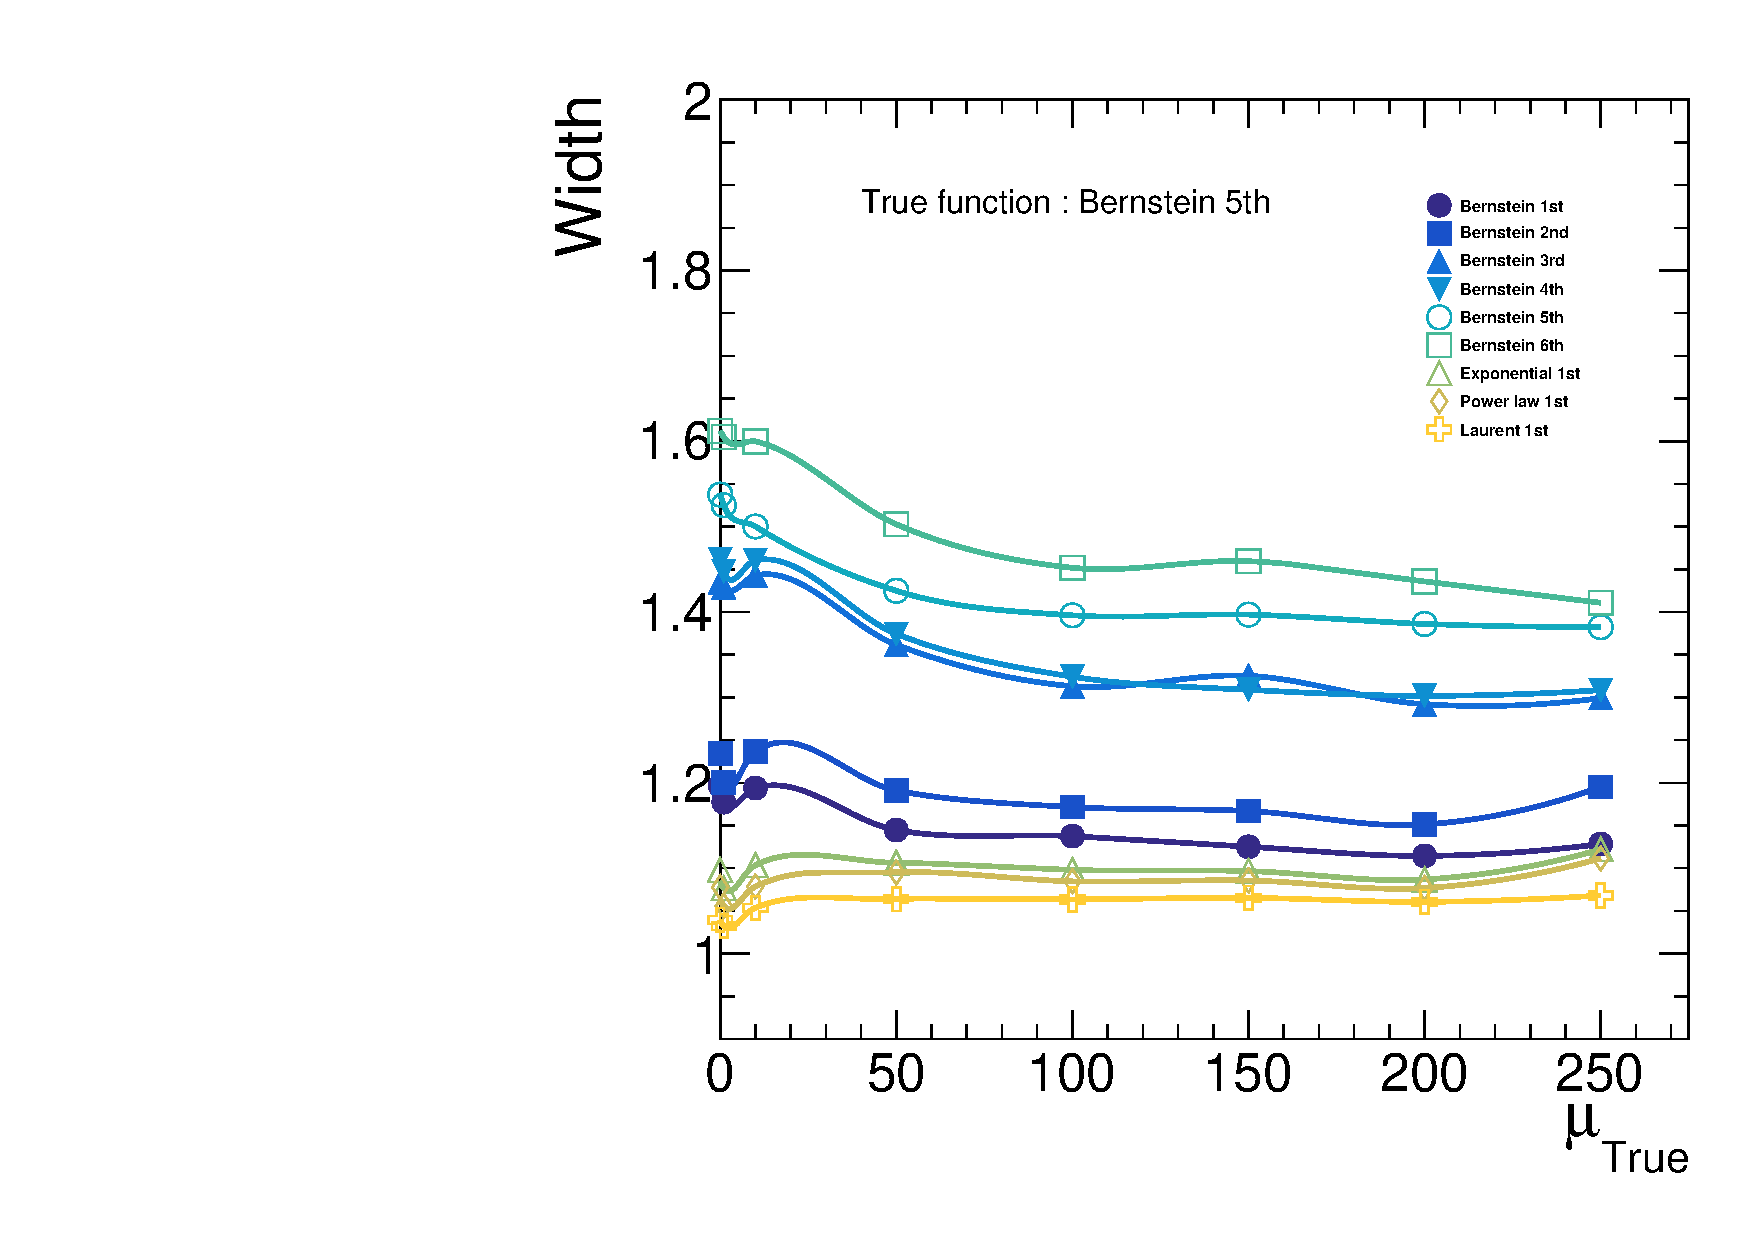
\includegraphics[width=0.33\textwidth]{Fig/BiasStudy/Linearity/ZJpsiG_Cat1/pull_width_linearity_TrueFunc4}~
  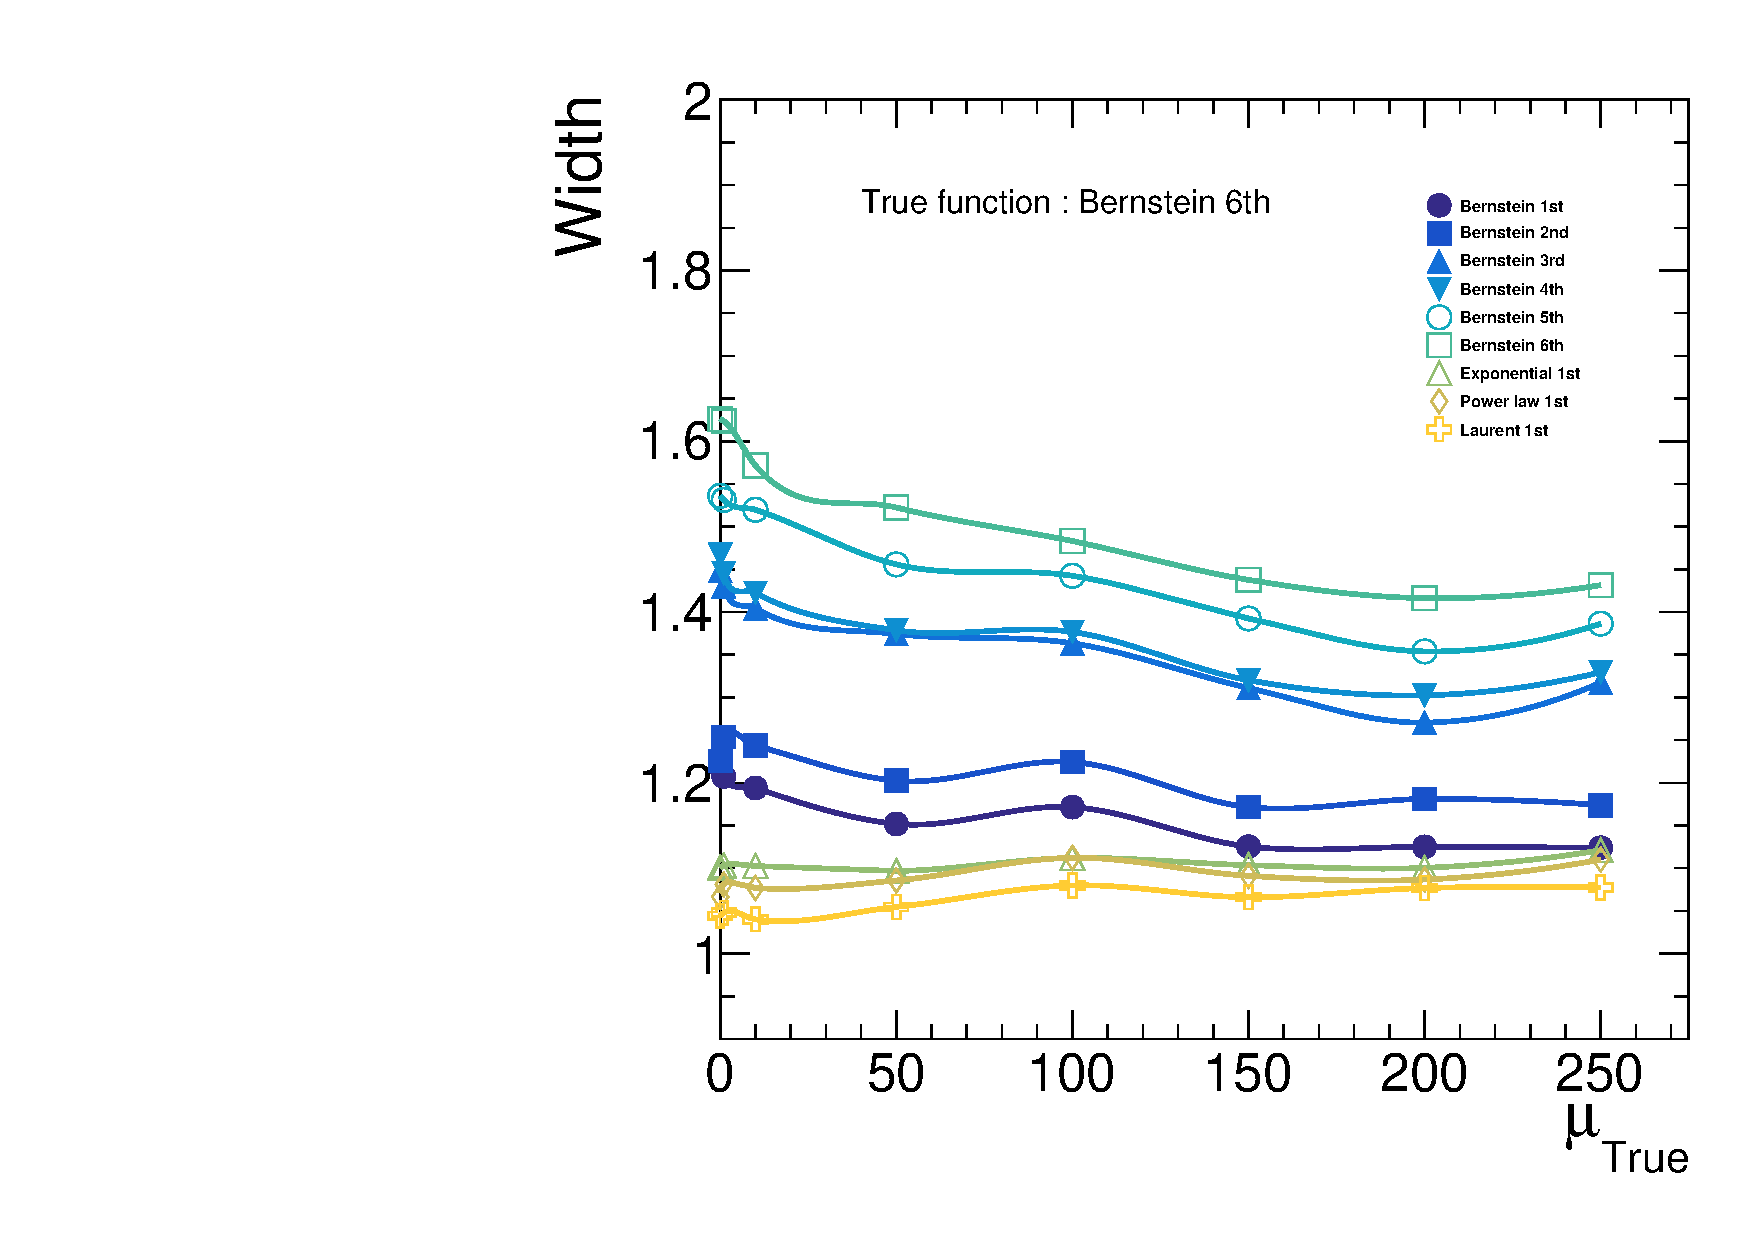
\includegraphics[width=0.33\textwidth]{Fig/BiasStudy/Linearity/ZJpsiG_Cat1/pull_width_linearity_TrueFunc5}\\
  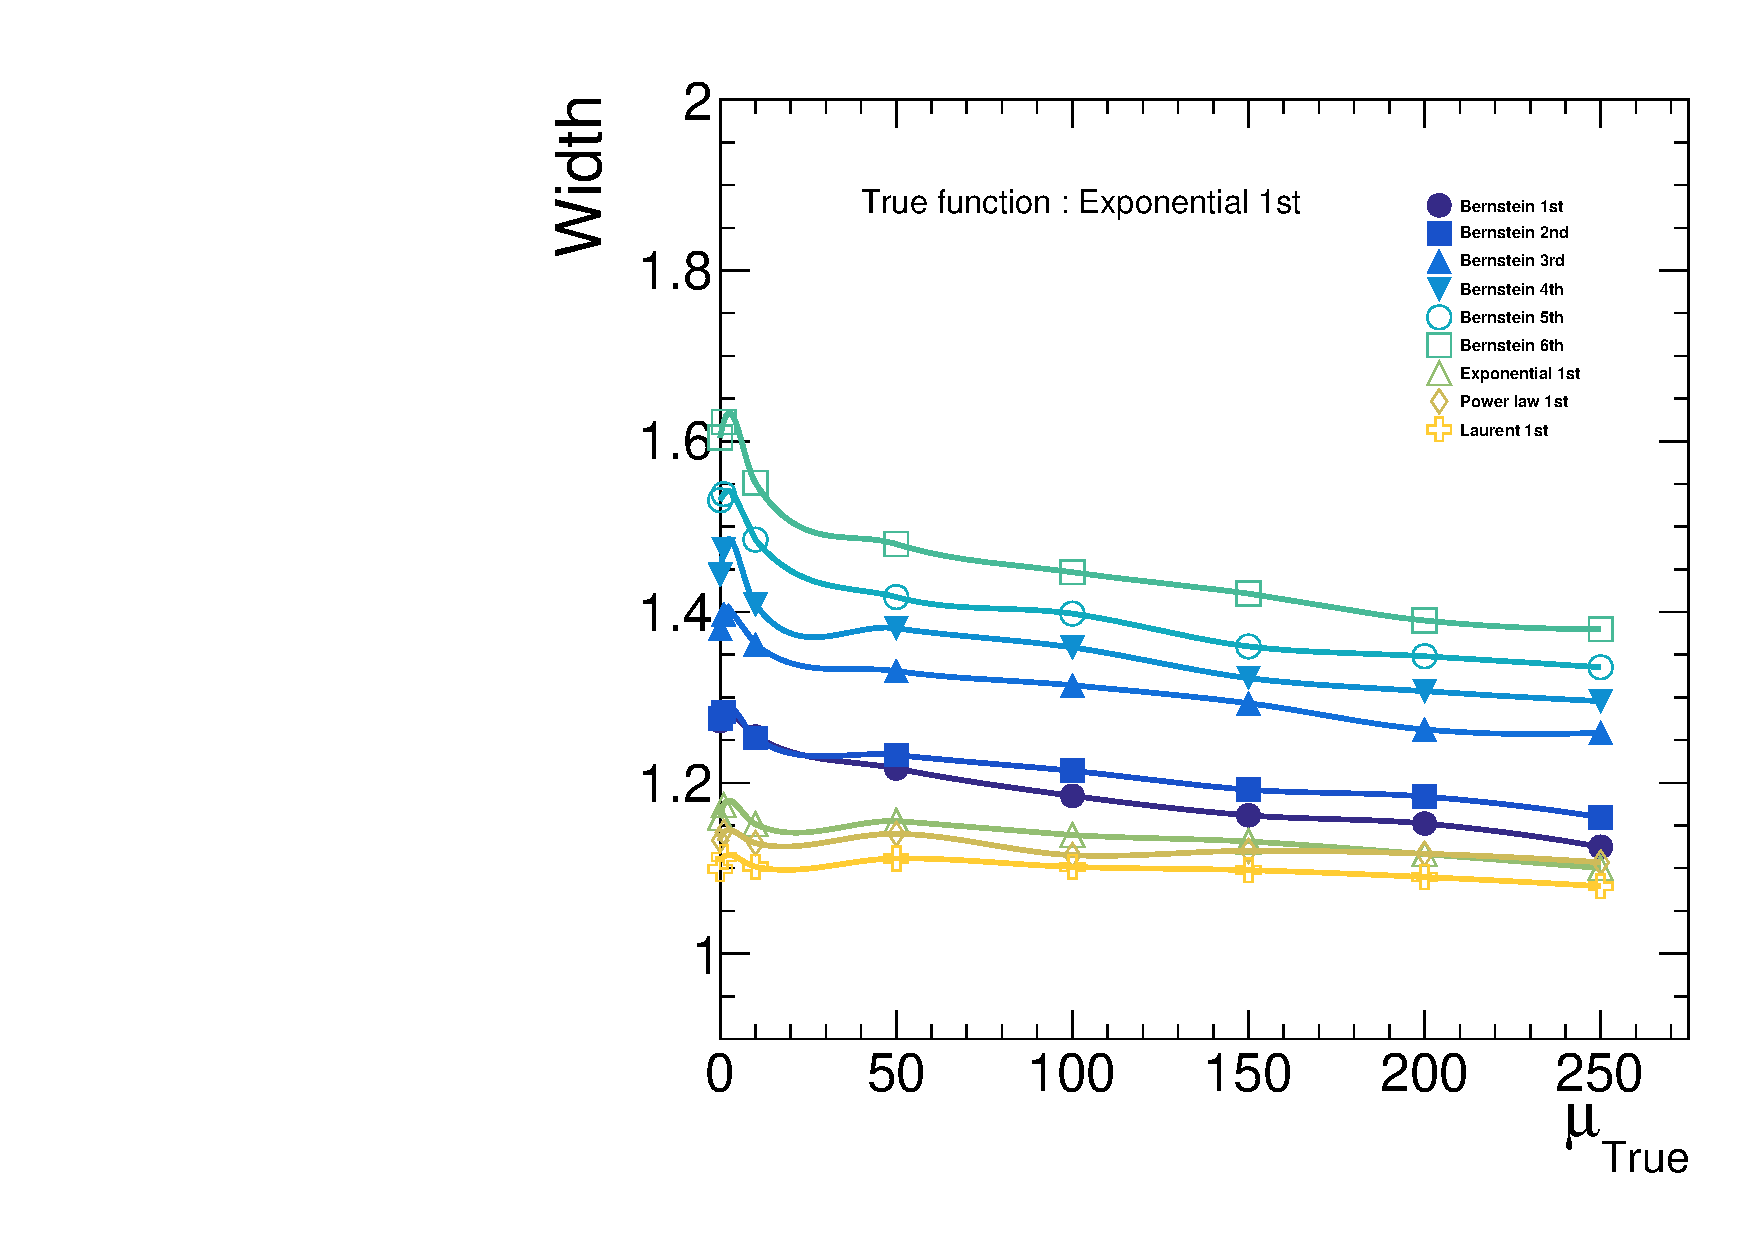
\includegraphics[width=0.33\textwidth]{Fig/BiasStudy/Linearity/ZJpsiG_Cat1/pull_width_linearity_TrueFunc6}~
  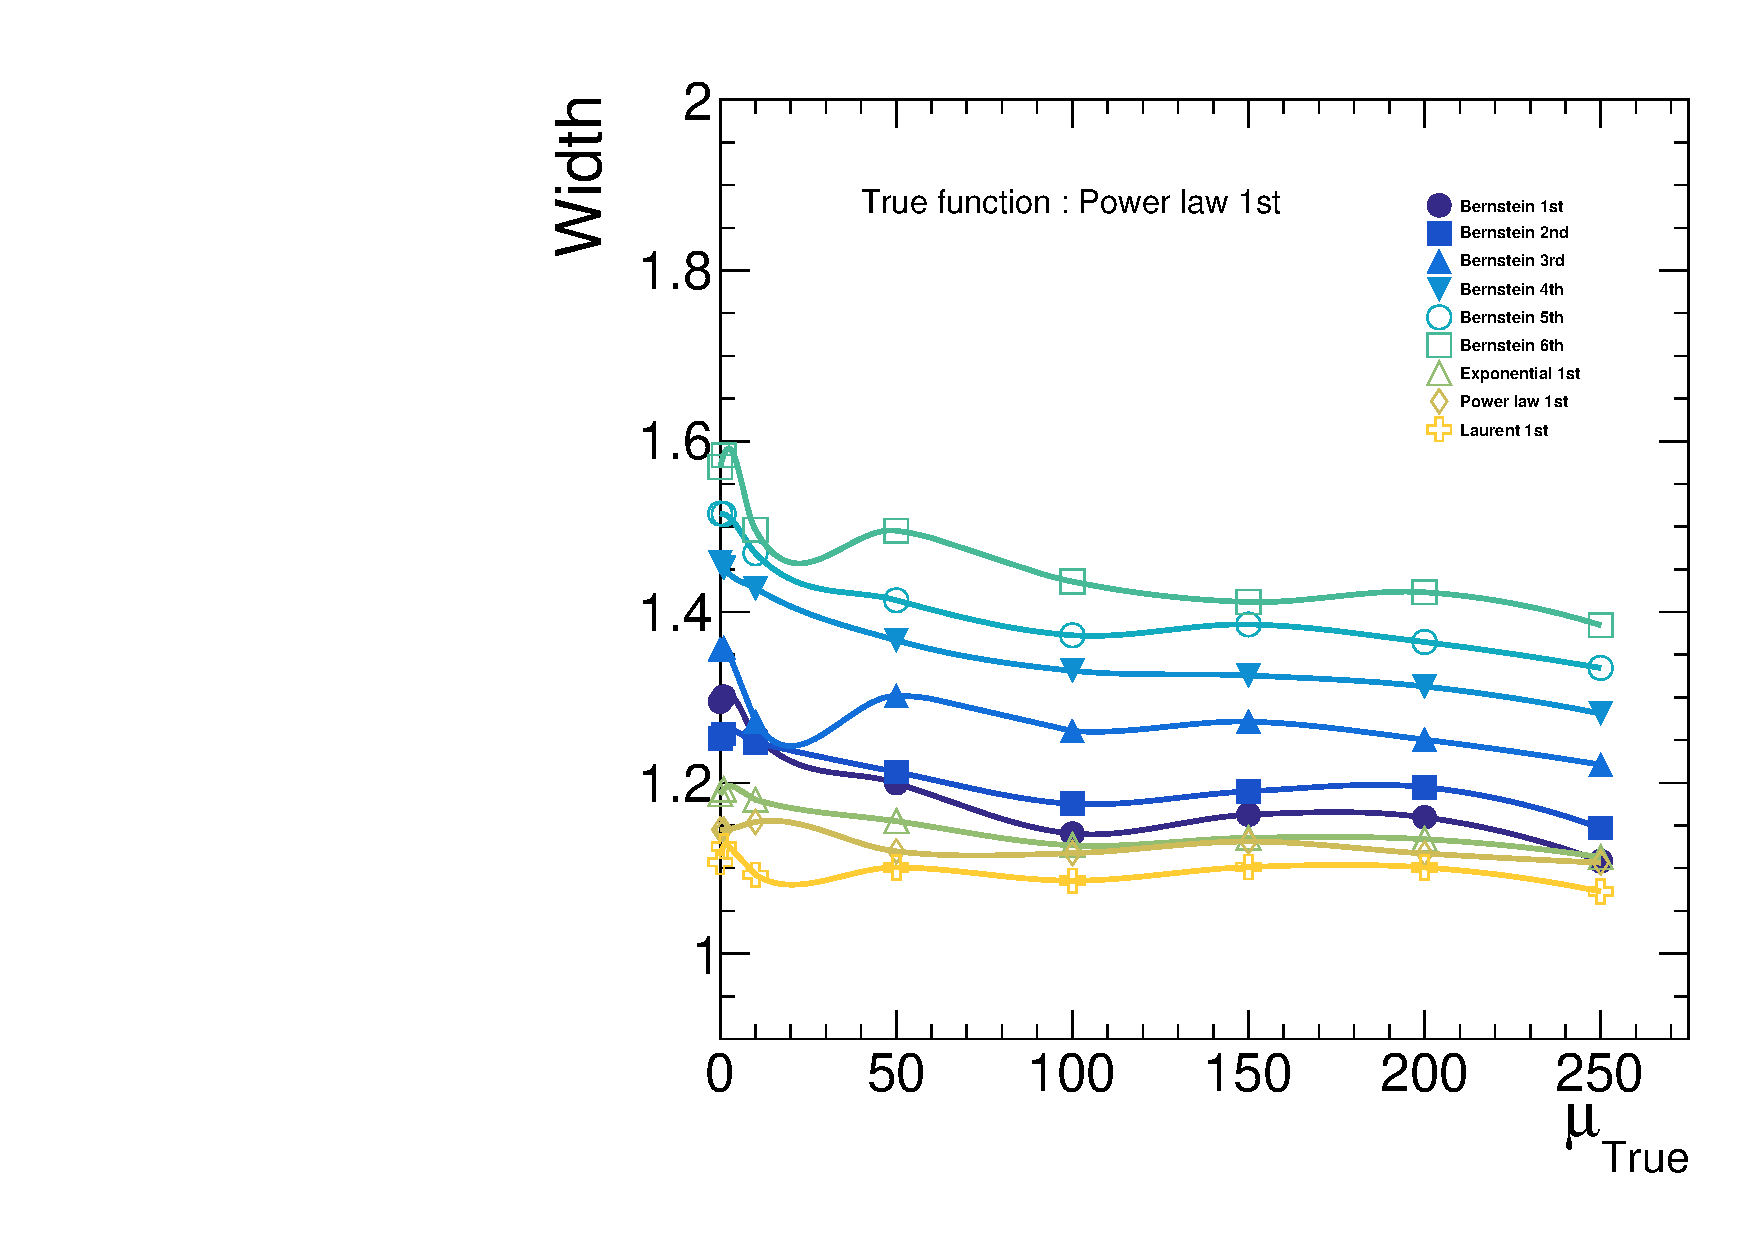
\includegraphics[width=0.33\textwidth]{Fig/BiasStudy/Linearity/ZJpsiG_Cat1/pull_width_linearity_TrueFunc7}~
  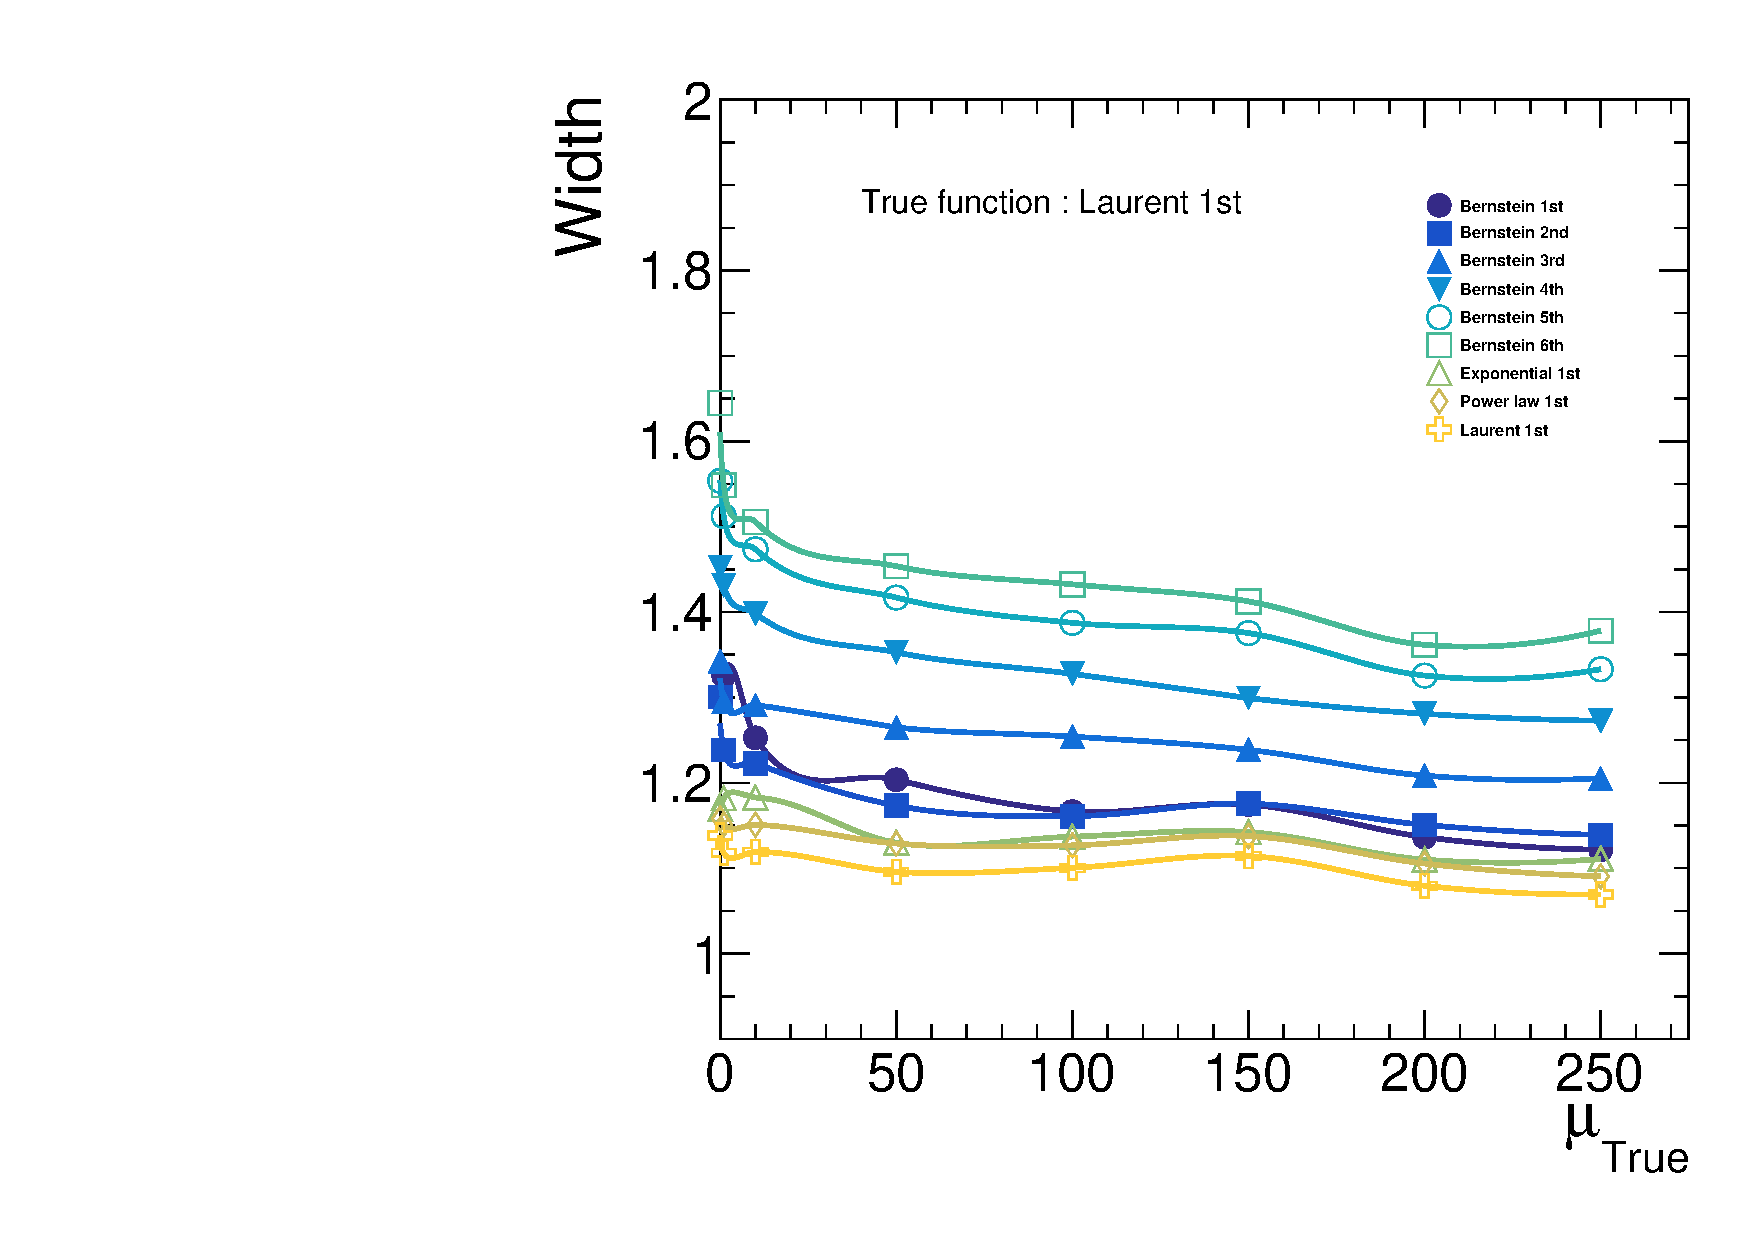
\includegraphics[width=0.33\textwidth]{Fig/BiasStudy/Linearity/ZJpsiG_Cat1/pull_width_linearity_TrueFunc8}\\
  \caption{The evolution of the width of the pull value distribution as more signal events are introduced in the Cat1 of the Z decay.}
  \label{fig:Linearity_width_ZJpsiG_Cat1}
\end{figure}
\clearpage
%
%
\subsection{$Z\to \JPsi\ \gamma$ Cat2}
\begin{figure}[!ht]
  \centering
  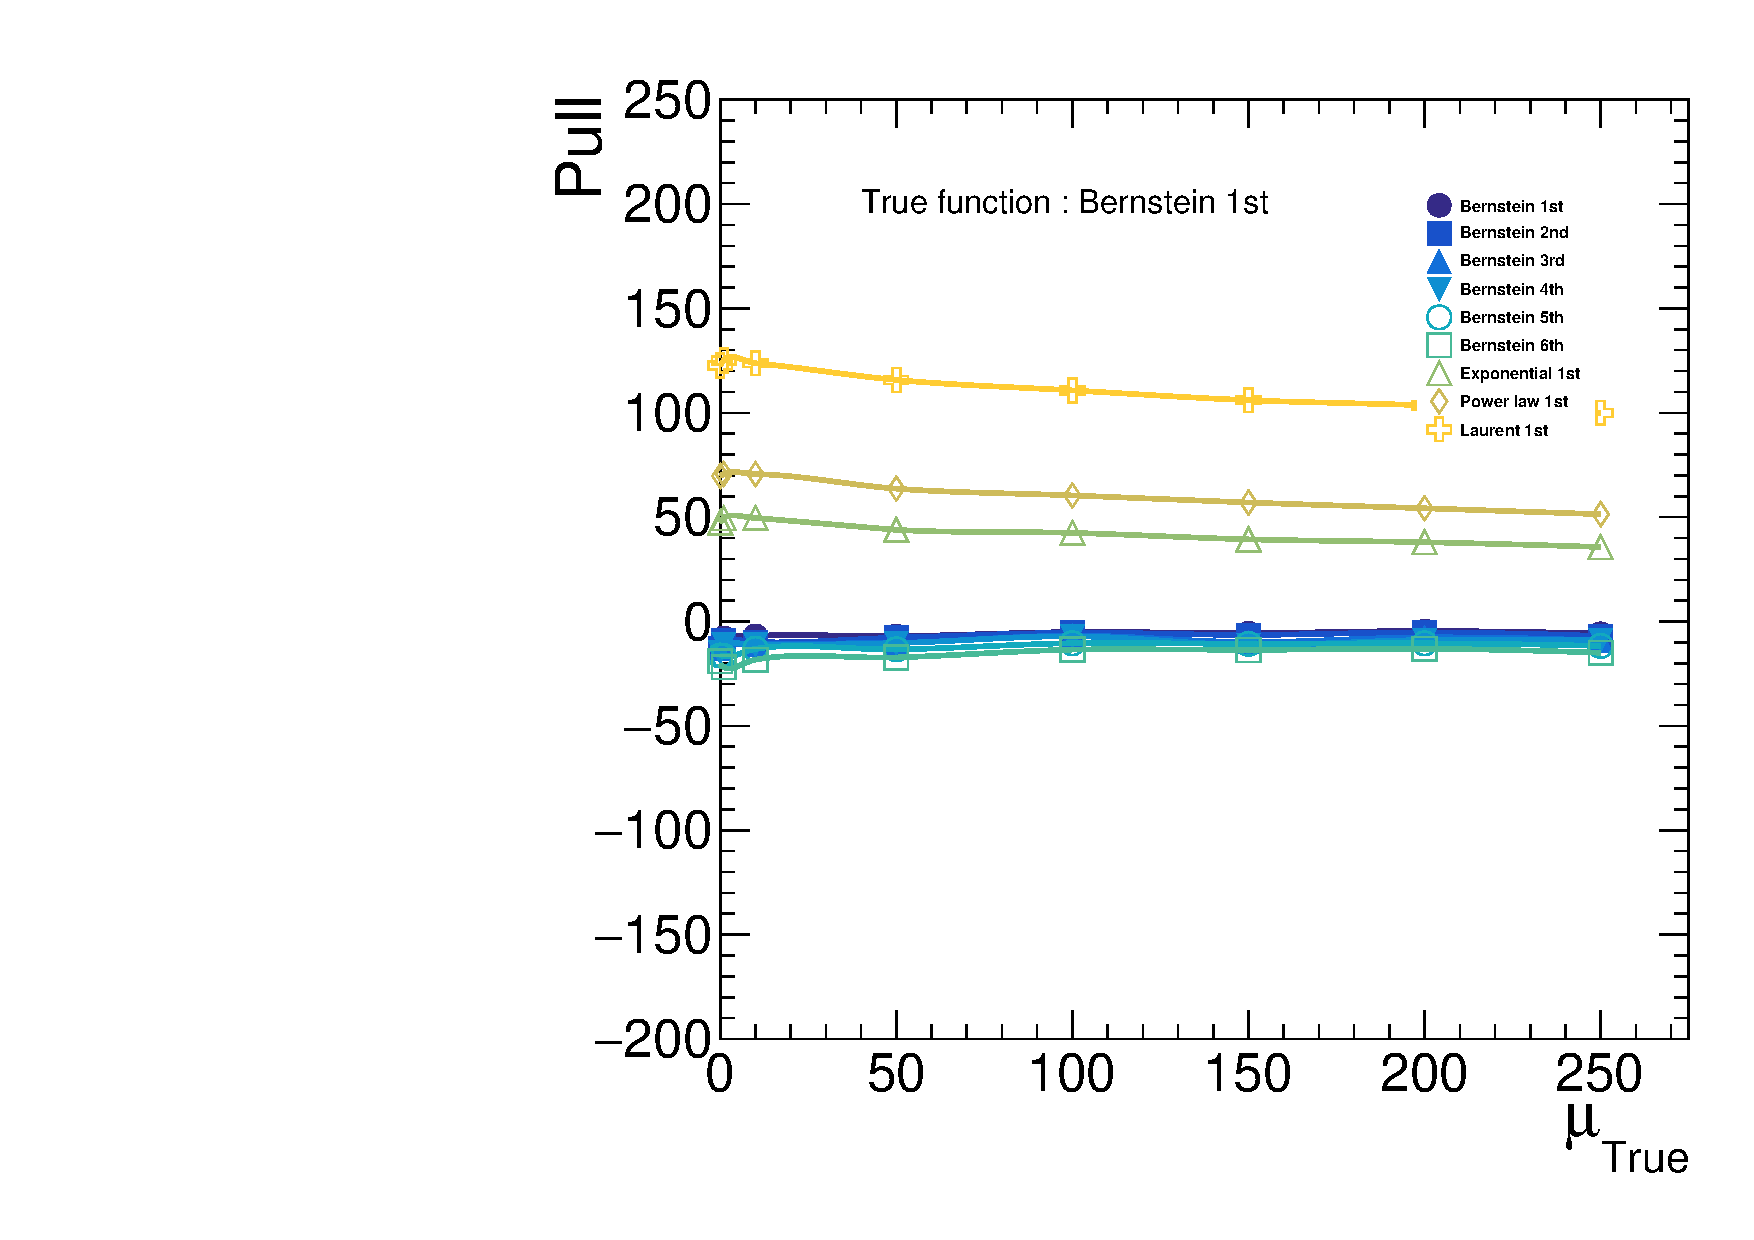
\includegraphics[width=0.33\textwidth]{Fig/BiasStudy/Linearity/ZJpsiG_Cat2/pull_mean_linearity_TrueFunc0}~
  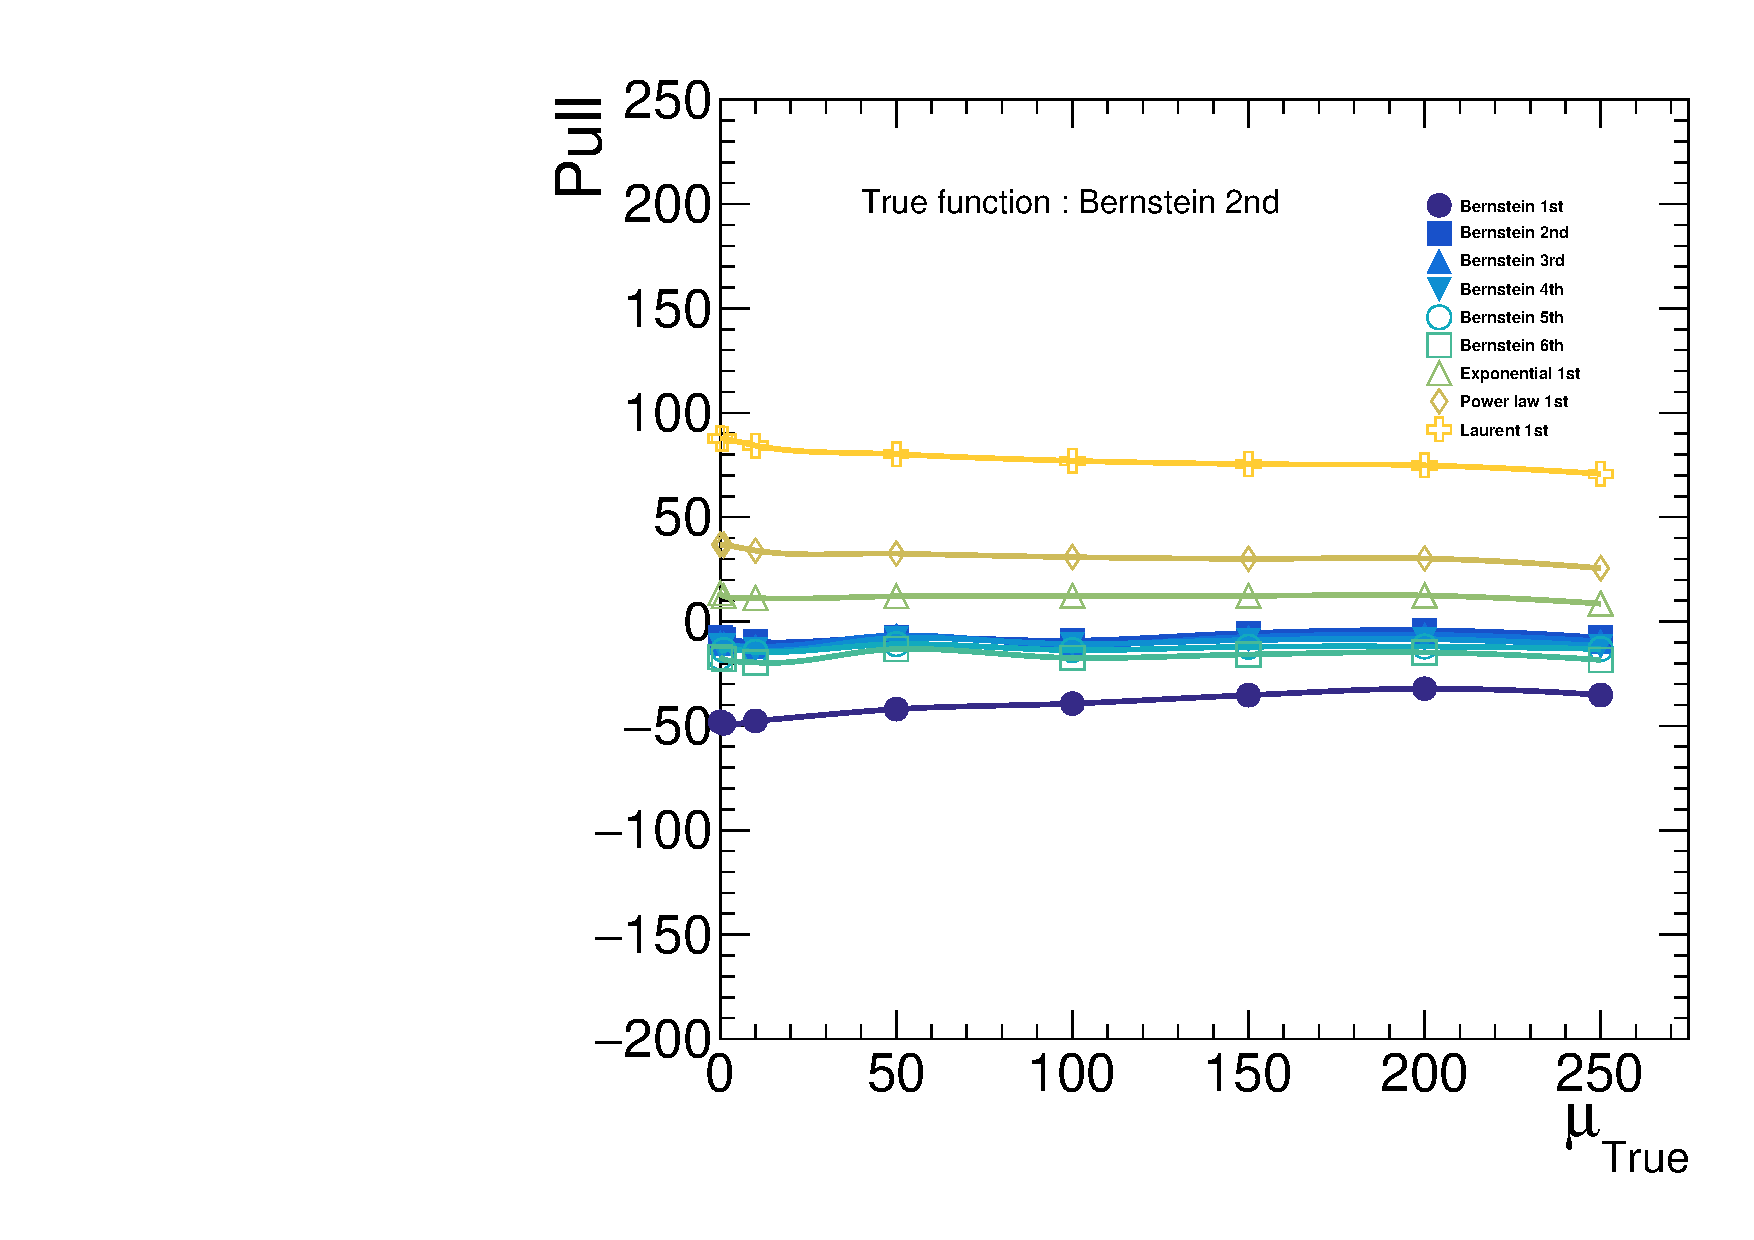
\includegraphics[width=0.33\textwidth]{Fig/BiasStudy/Linearity/ZJpsiG_Cat2/pull_mean_linearity_TrueFunc1}~
  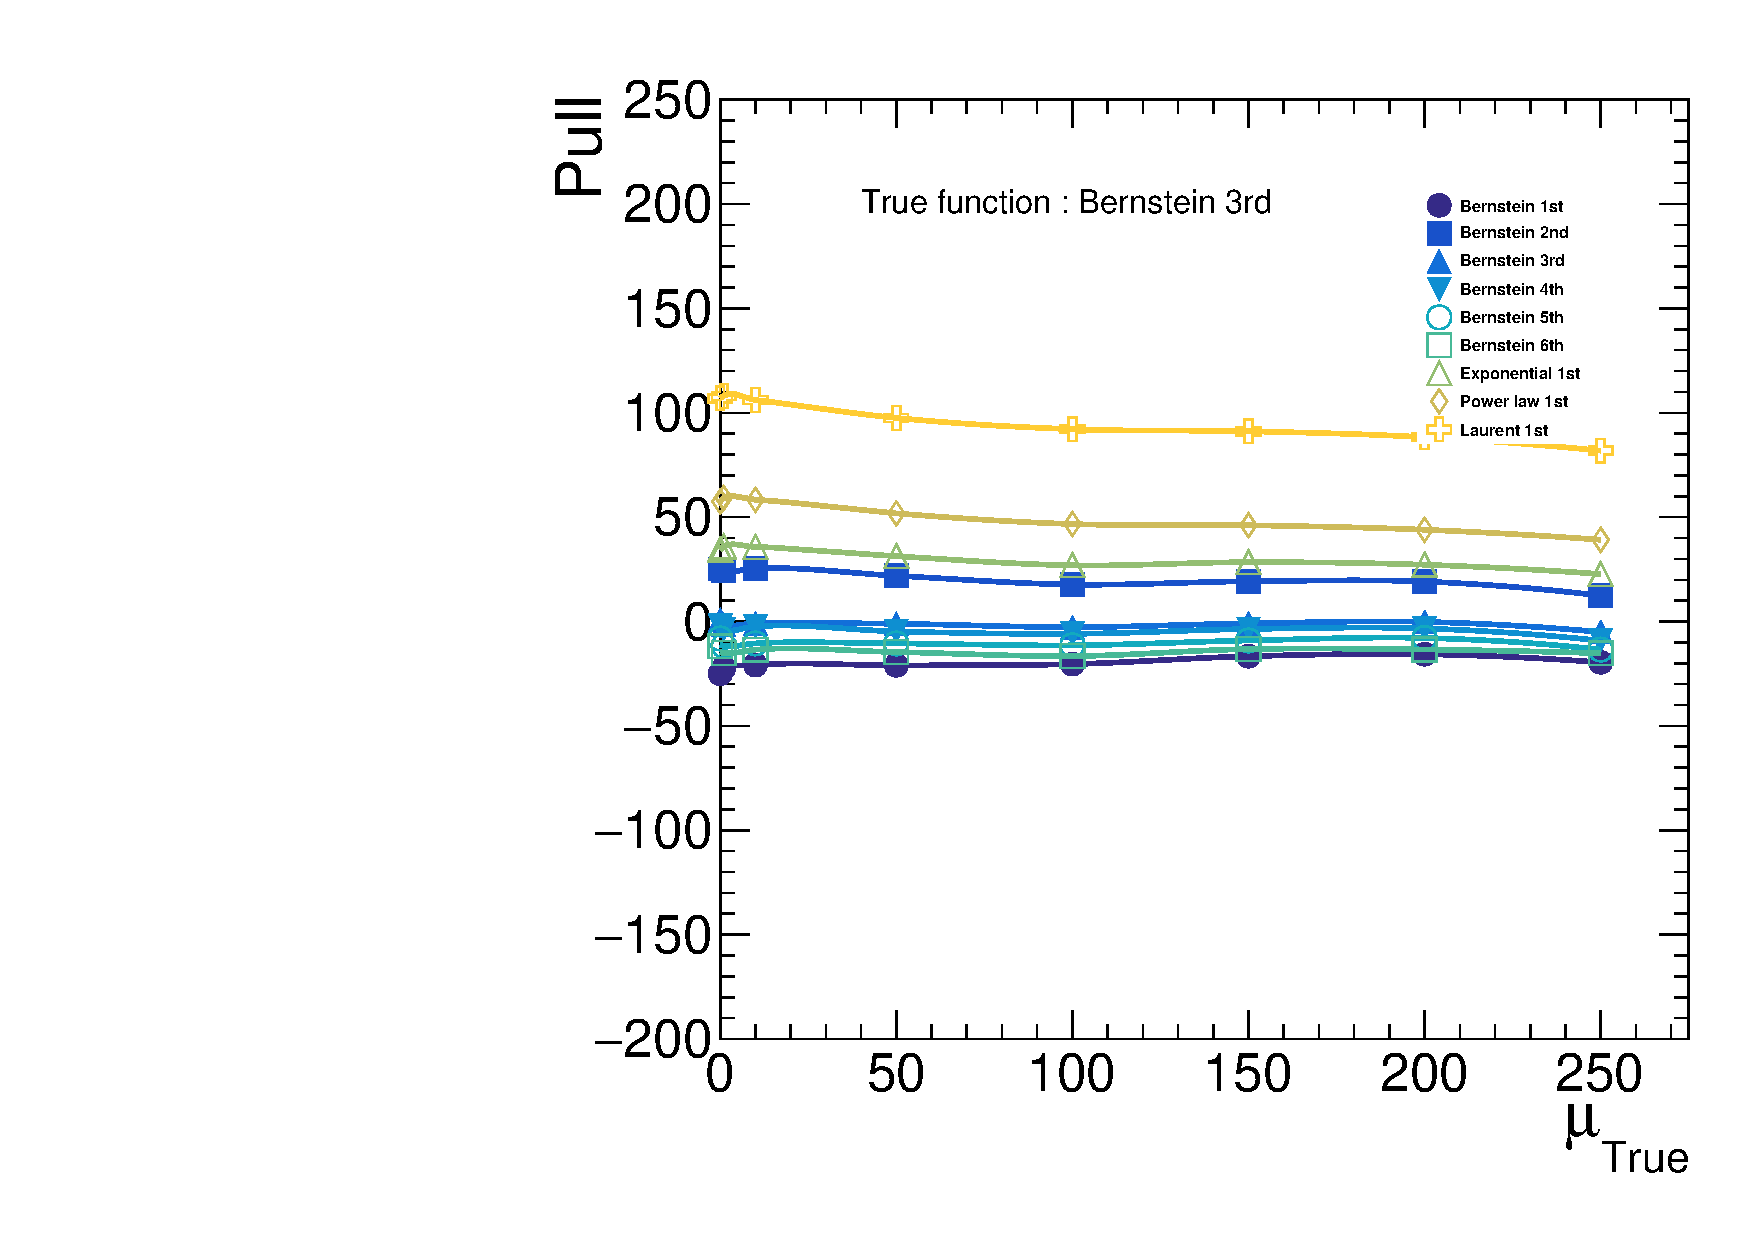
\includegraphics[width=0.33\textwidth]{Fig/BiasStudy/Linearity/ZJpsiG_Cat2/pull_mean_linearity_TrueFunc2}\\
  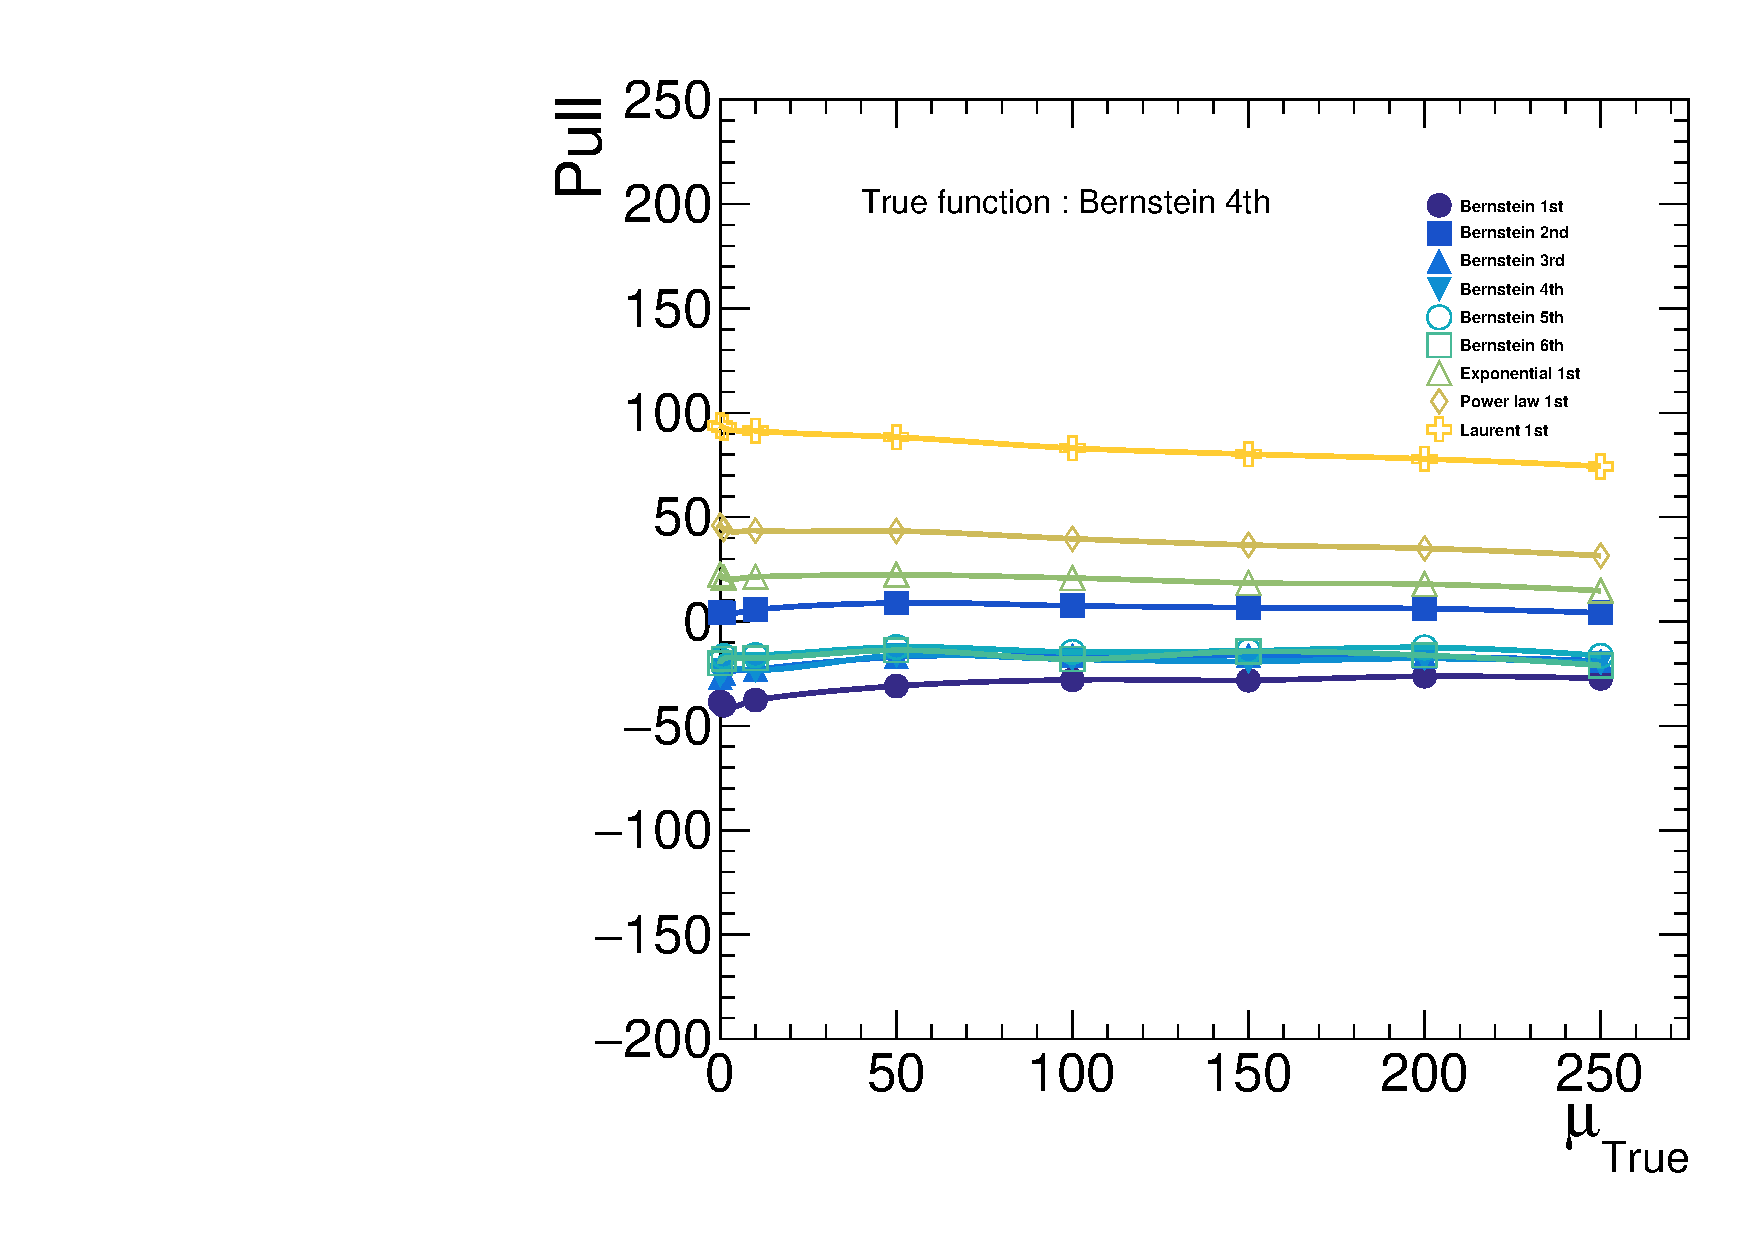
\includegraphics[width=0.33\textwidth]{Fig/BiasStudy/Linearity/ZJpsiG_Cat2/pull_mean_linearity_TrueFunc3}~
  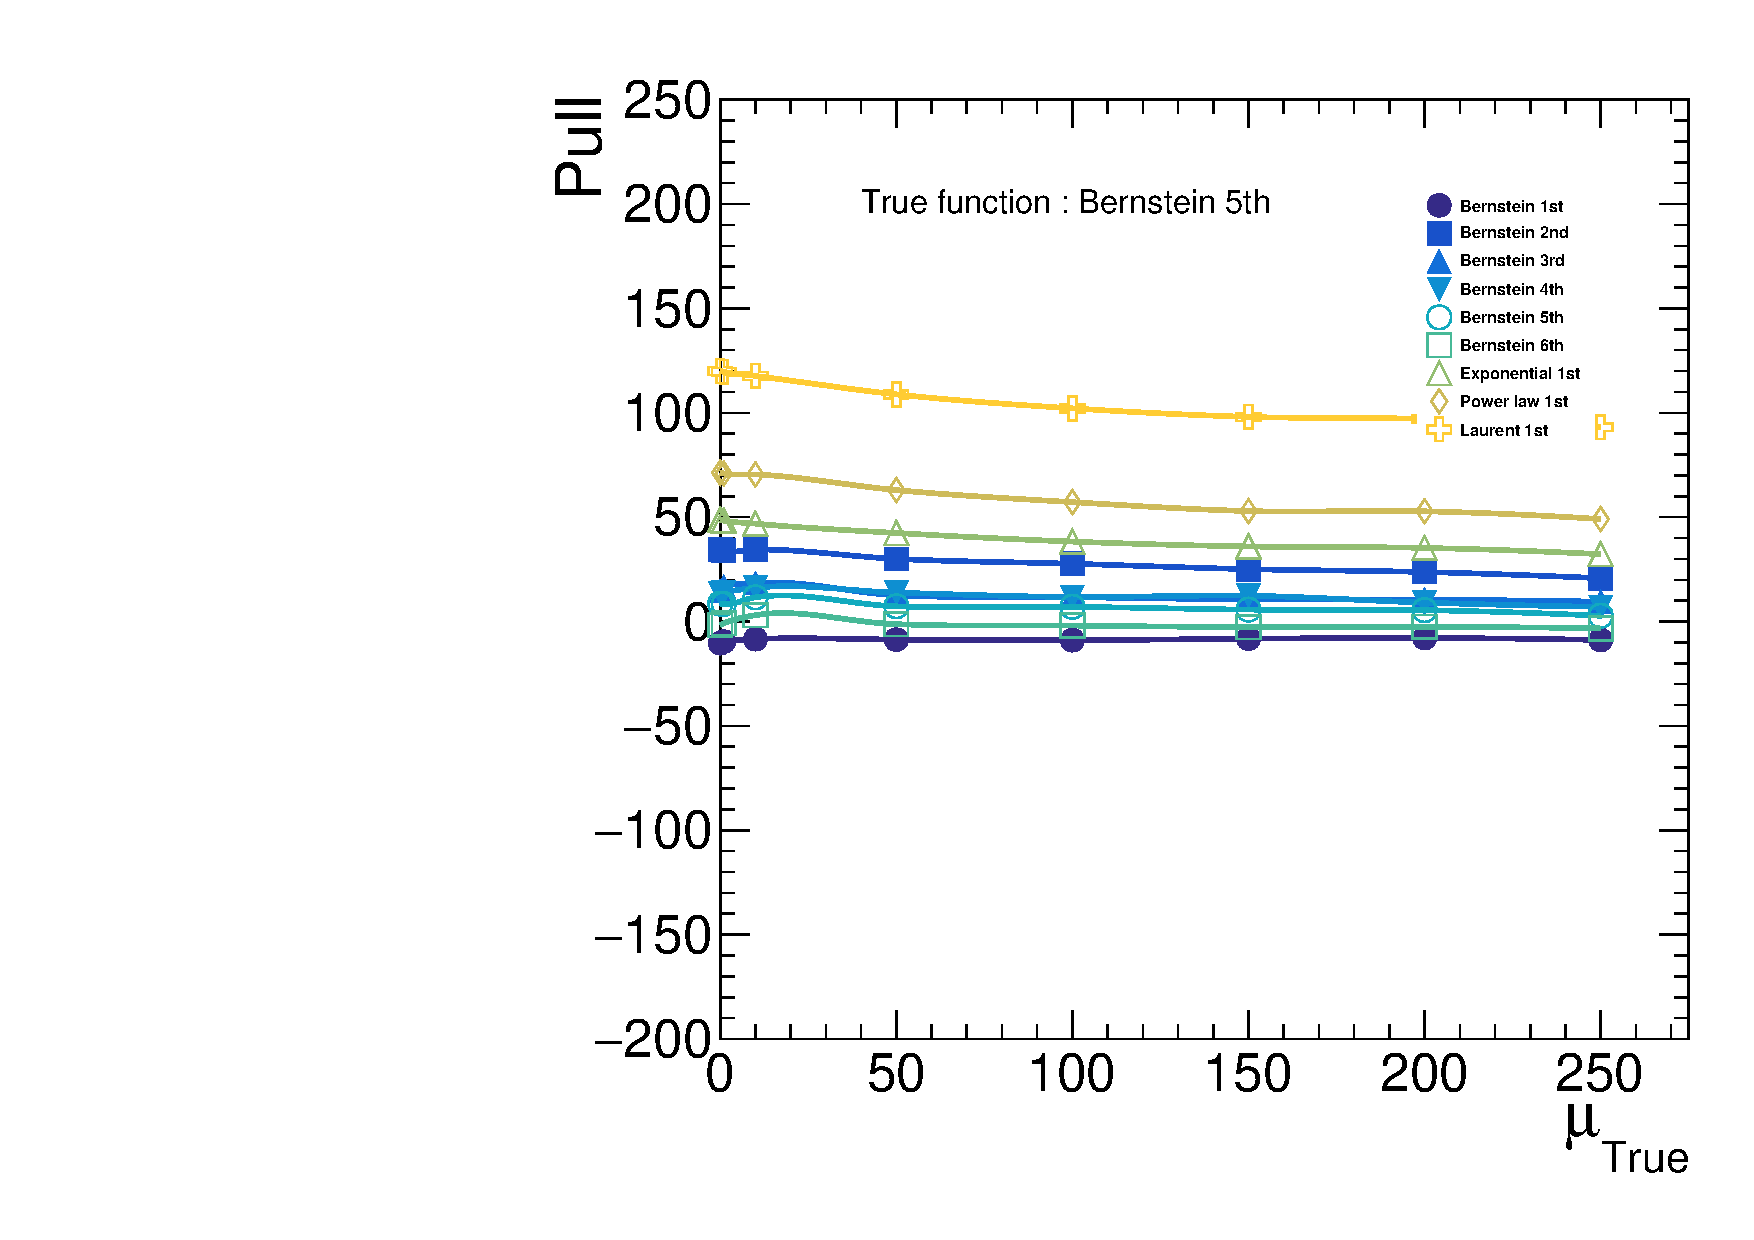
\includegraphics[width=0.33\textwidth]{Fig/BiasStudy/Linearity/ZJpsiG_Cat2/pull_mean_linearity_TrueFunc4}~
  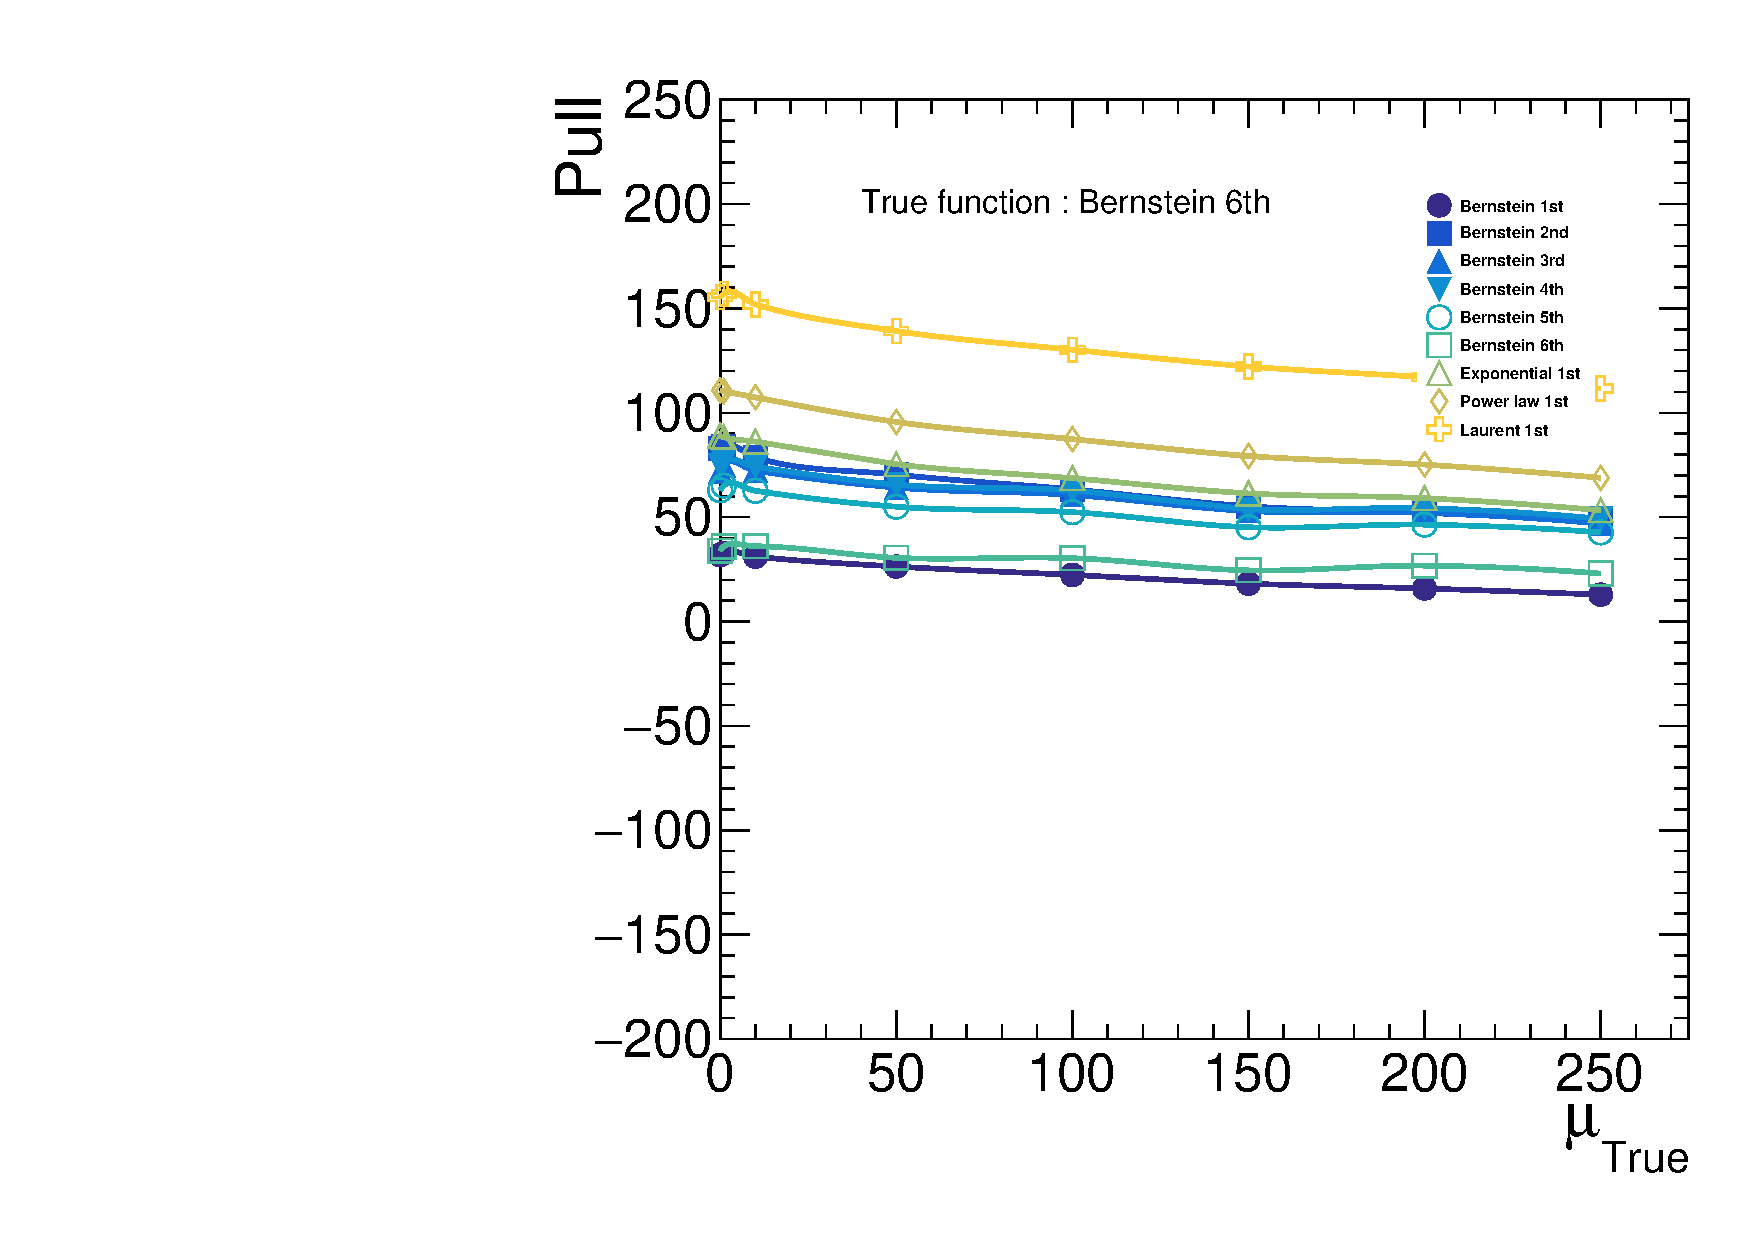
\includegraphics[width=0.33\textwidth]{Fig/BiasStudy/Linearity/ZJpsiG_Cat2/pull_mean_linearity_TrueFunc5}\\
  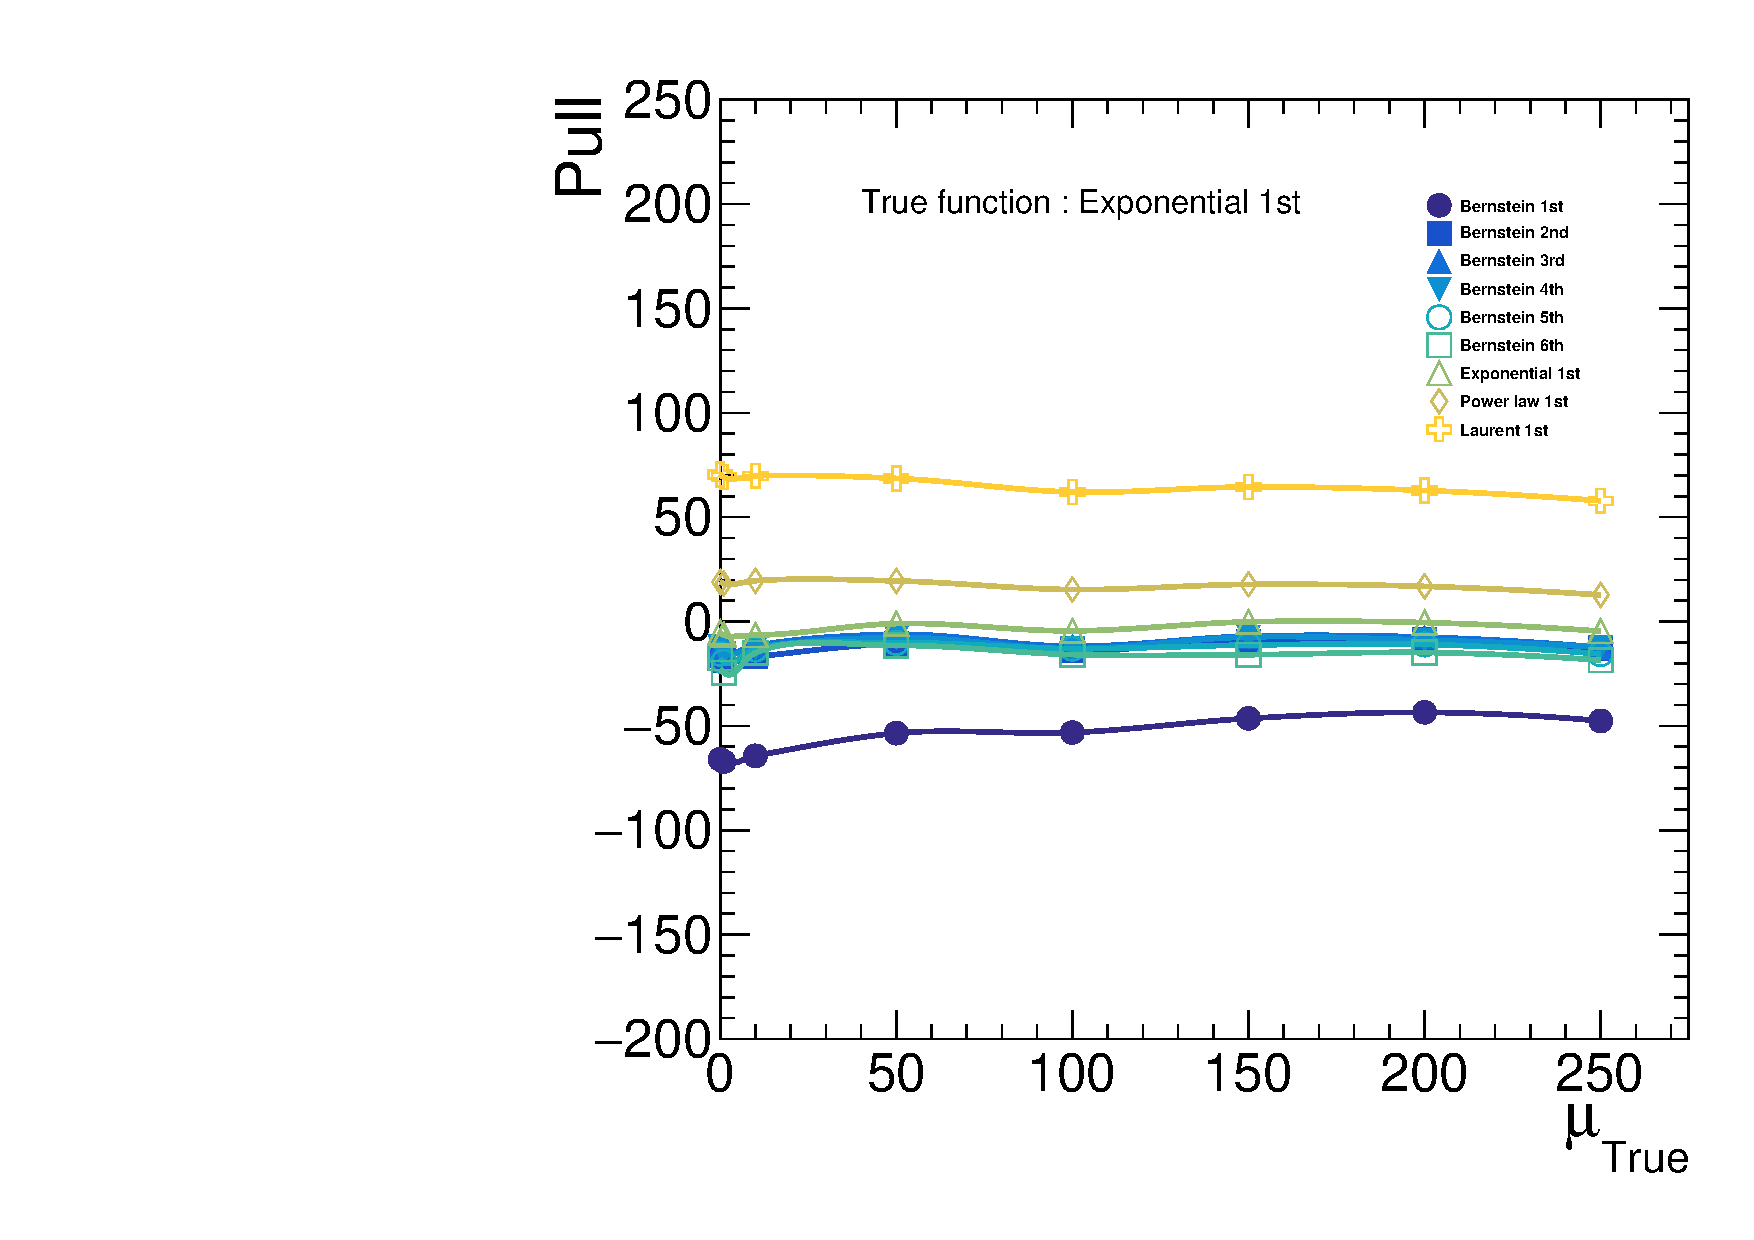
\includegraphics[width=0.33\textwidth]{Fig/BiasStudy/Linearity/ZJpsiG_Cat2/pull_mean_linearity_TrueFunc6}~
  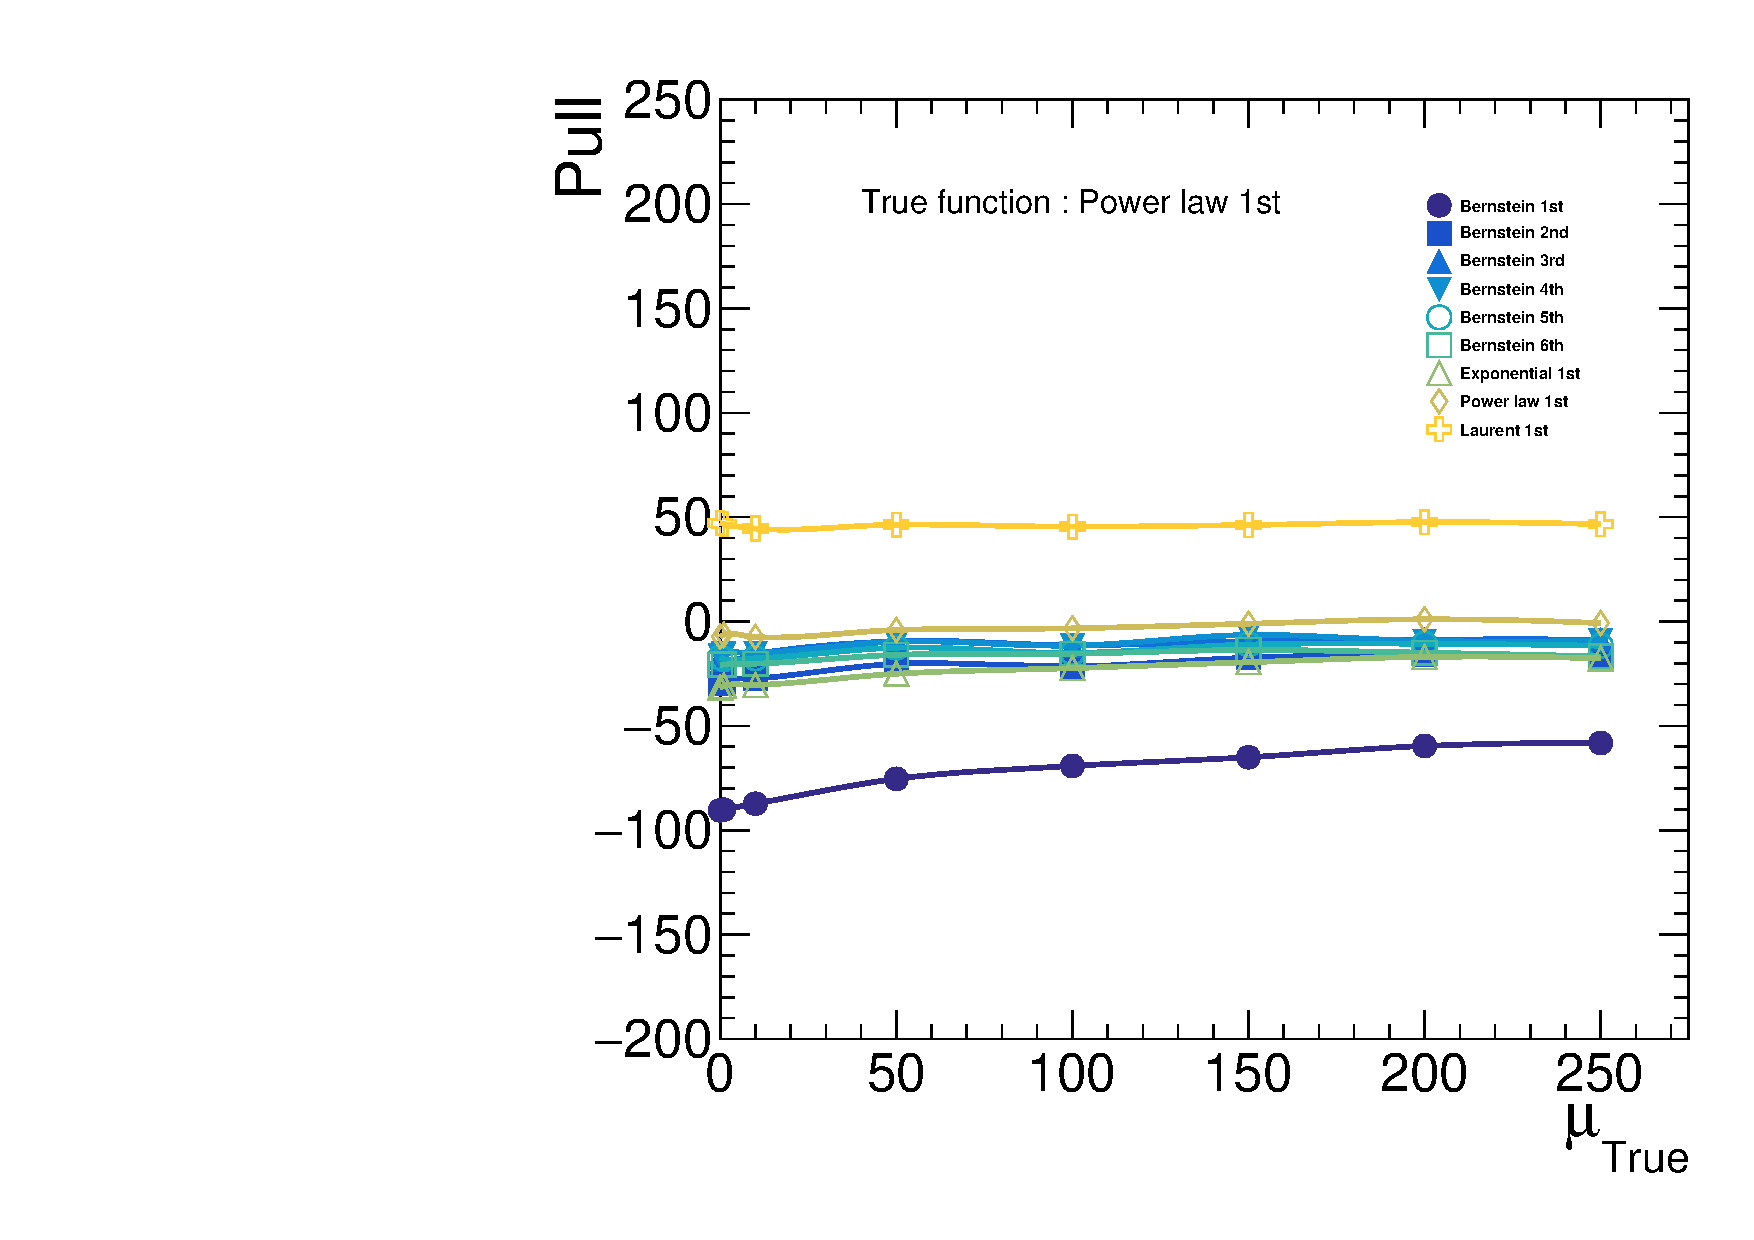
\includegraphics[width=0.33\textwidth]{Fig/BiasStudy/Linearity/ZJpsiG_Cat2/pull_mean_linearity_TrueFunc7}~
  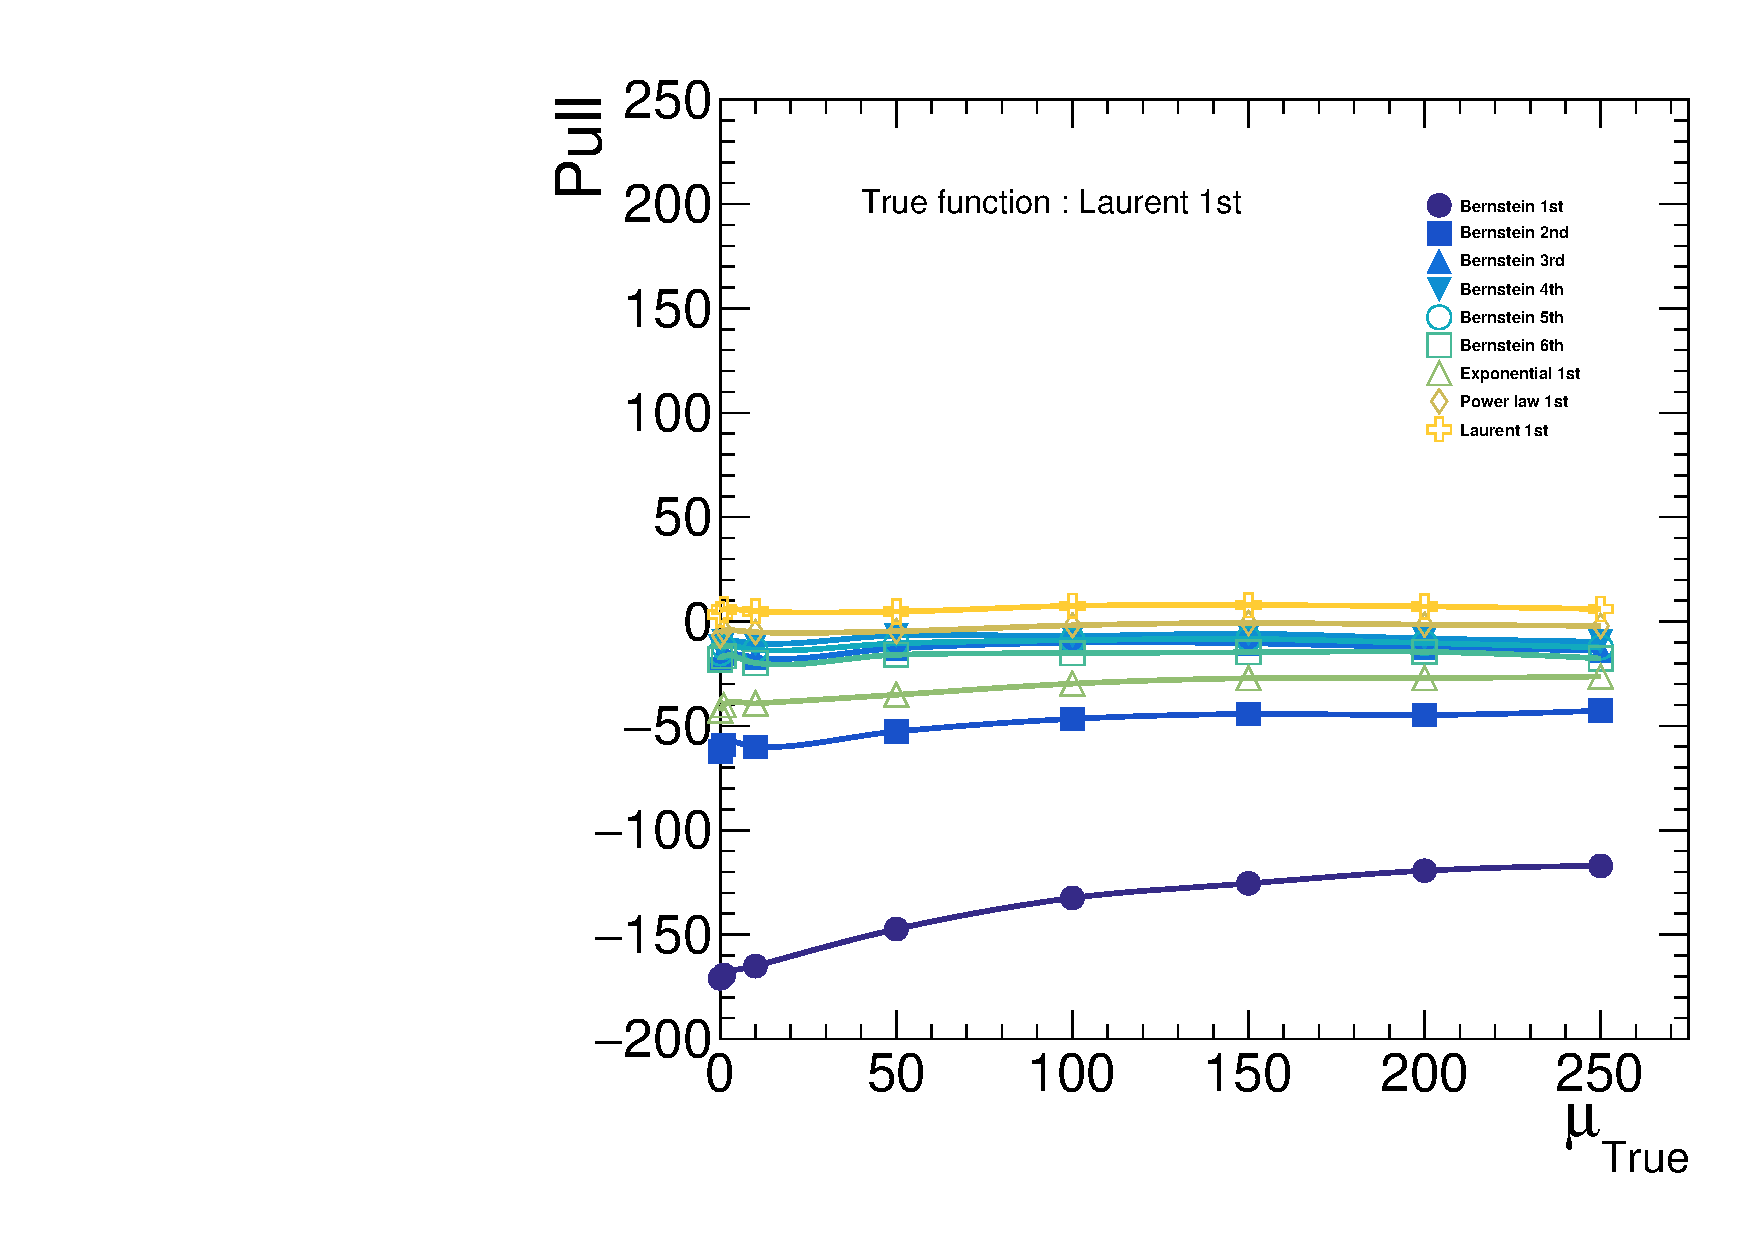
\includegraphics[width=0.33\textwidth]{Fig/BiasStudy/Linearity/ZJpsiG_Cat2/pull_mean_linearity_TrueFunc8}\\
  \caption{The evolution of the mean of the pull value distribution as more signal events are introduced in the Cat2 of the Z decay.}
  \label{fig:Linearity_mean_ZJpsiG_Cat2}
\end{figure}
\clearpage
%
\begin{figure}[!ht]
  \centering
  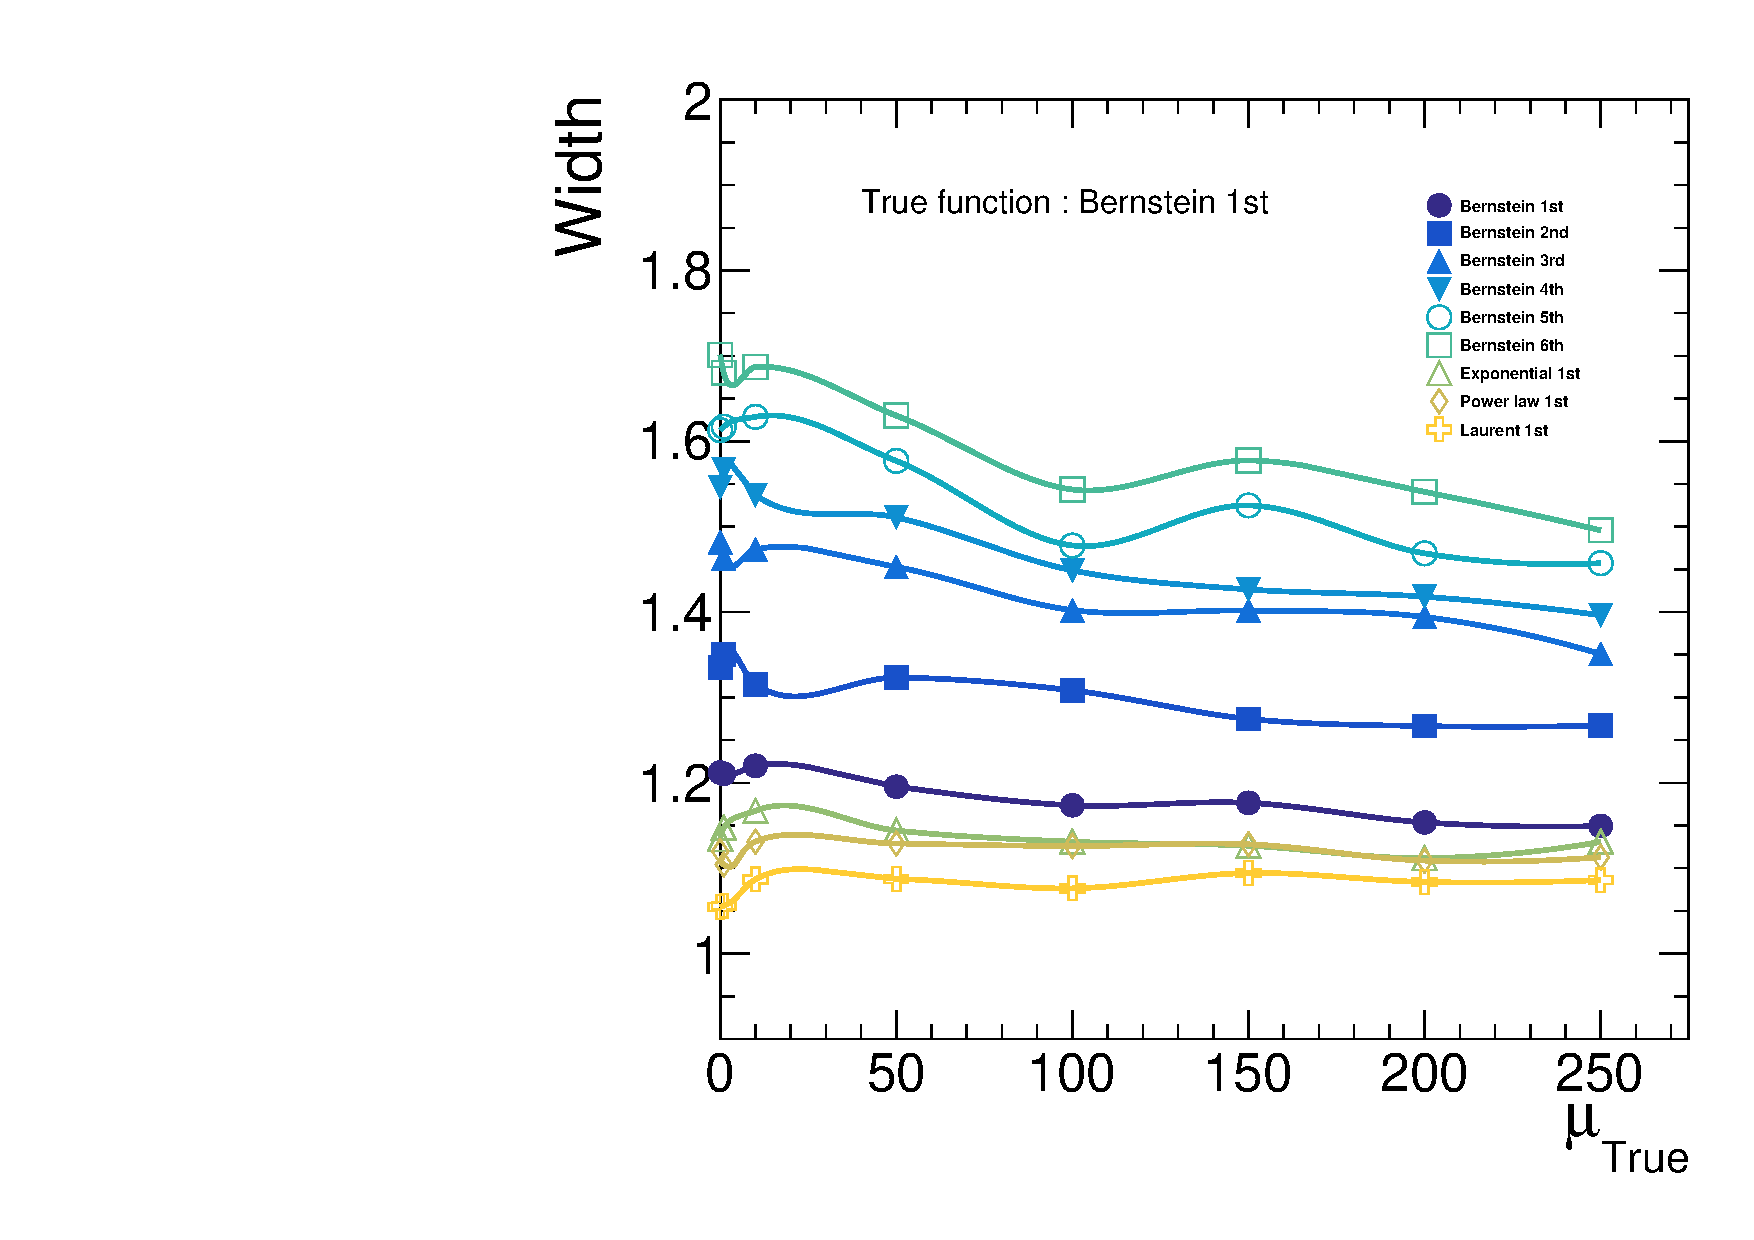
\includegraphics[width=0.33\textwidth]{Fig/BiasStudy/Linearity/ZJpsiG_Cat2/pull_width_linearity_TrueFunc0}~
  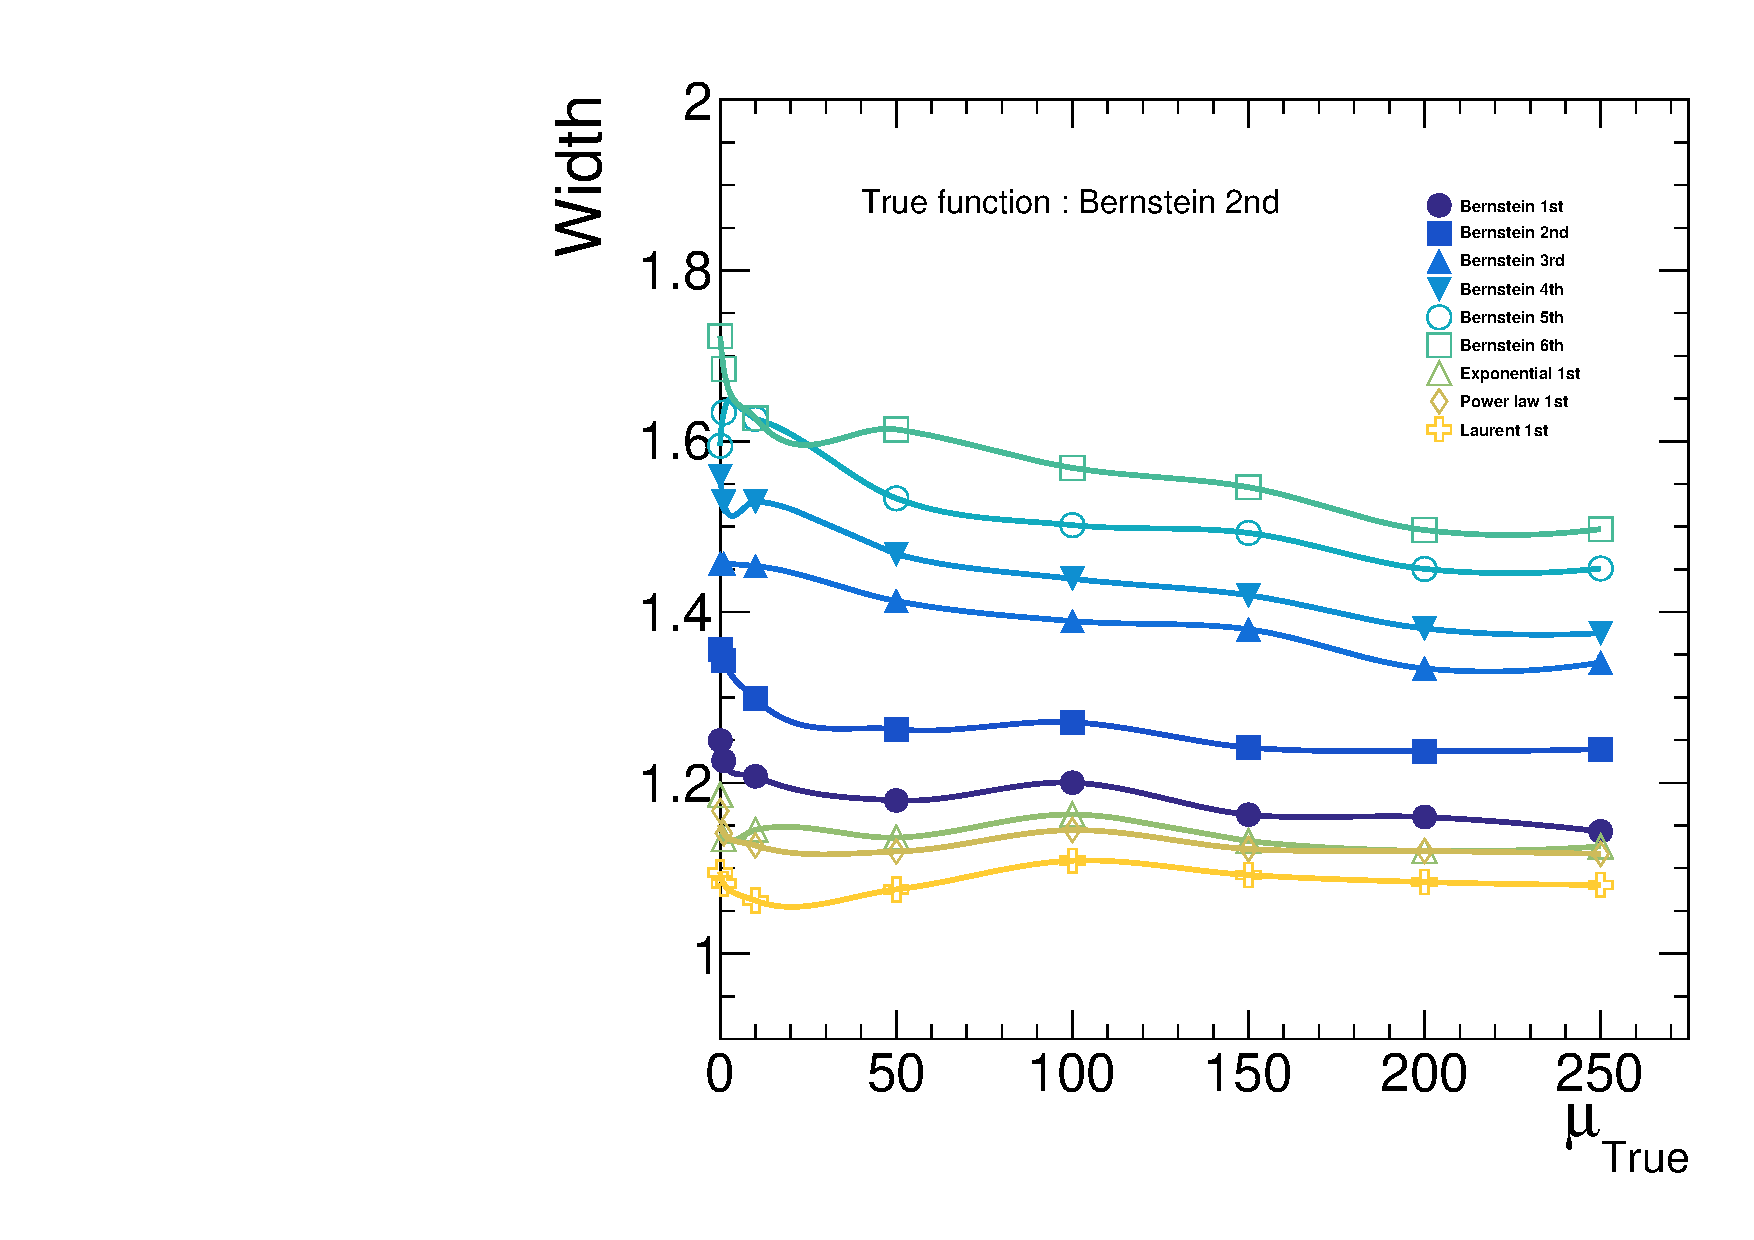
\includegraphics[width=0.33\textwidth]{Fig/BiasStudy/Linearity/ZJpsiG_Cat2/pull_width_linearity_TrueFunc1}~
  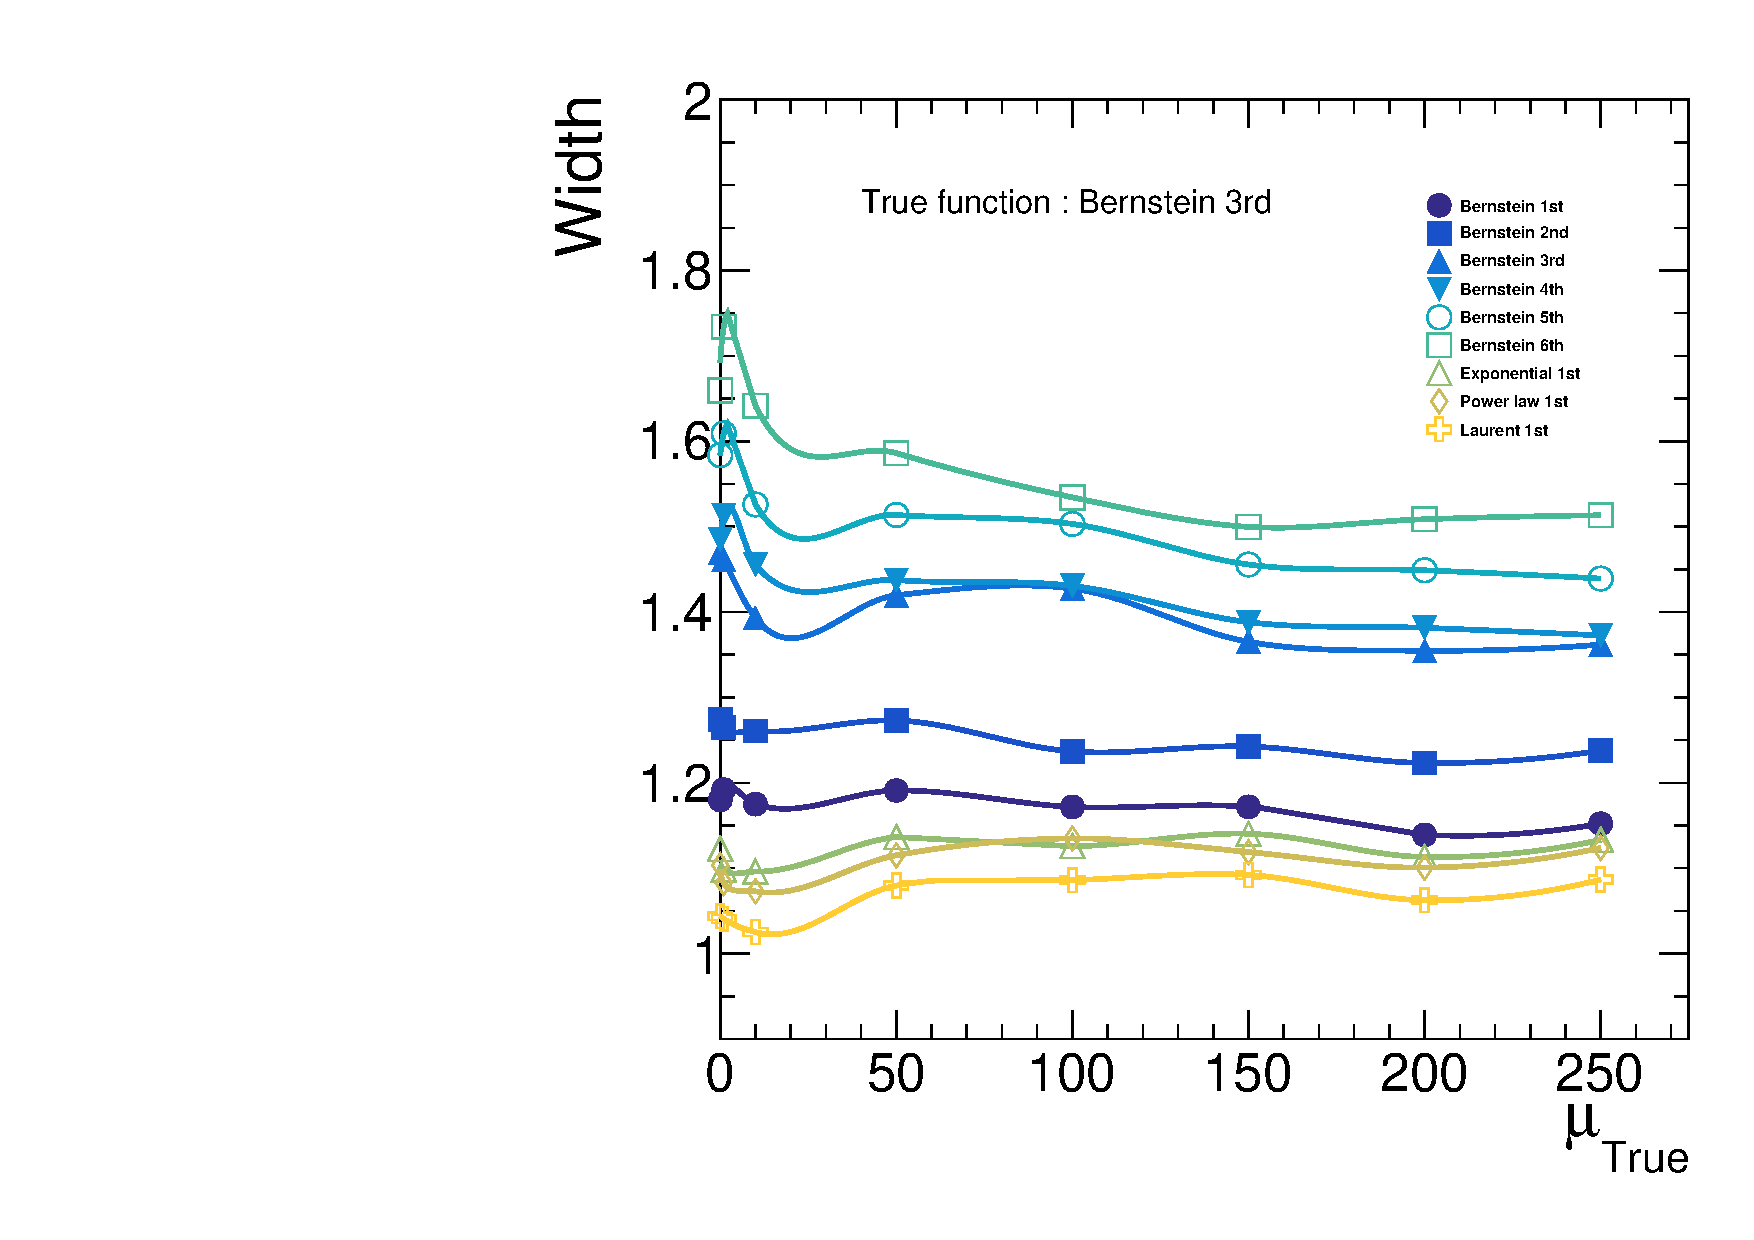
\includegraphics[width=0.33\textwidth]{Fig/BiasStudy/Linearity/ZJpsiG_Cat2/pull_width_linearity_TrueFunc2}\\
  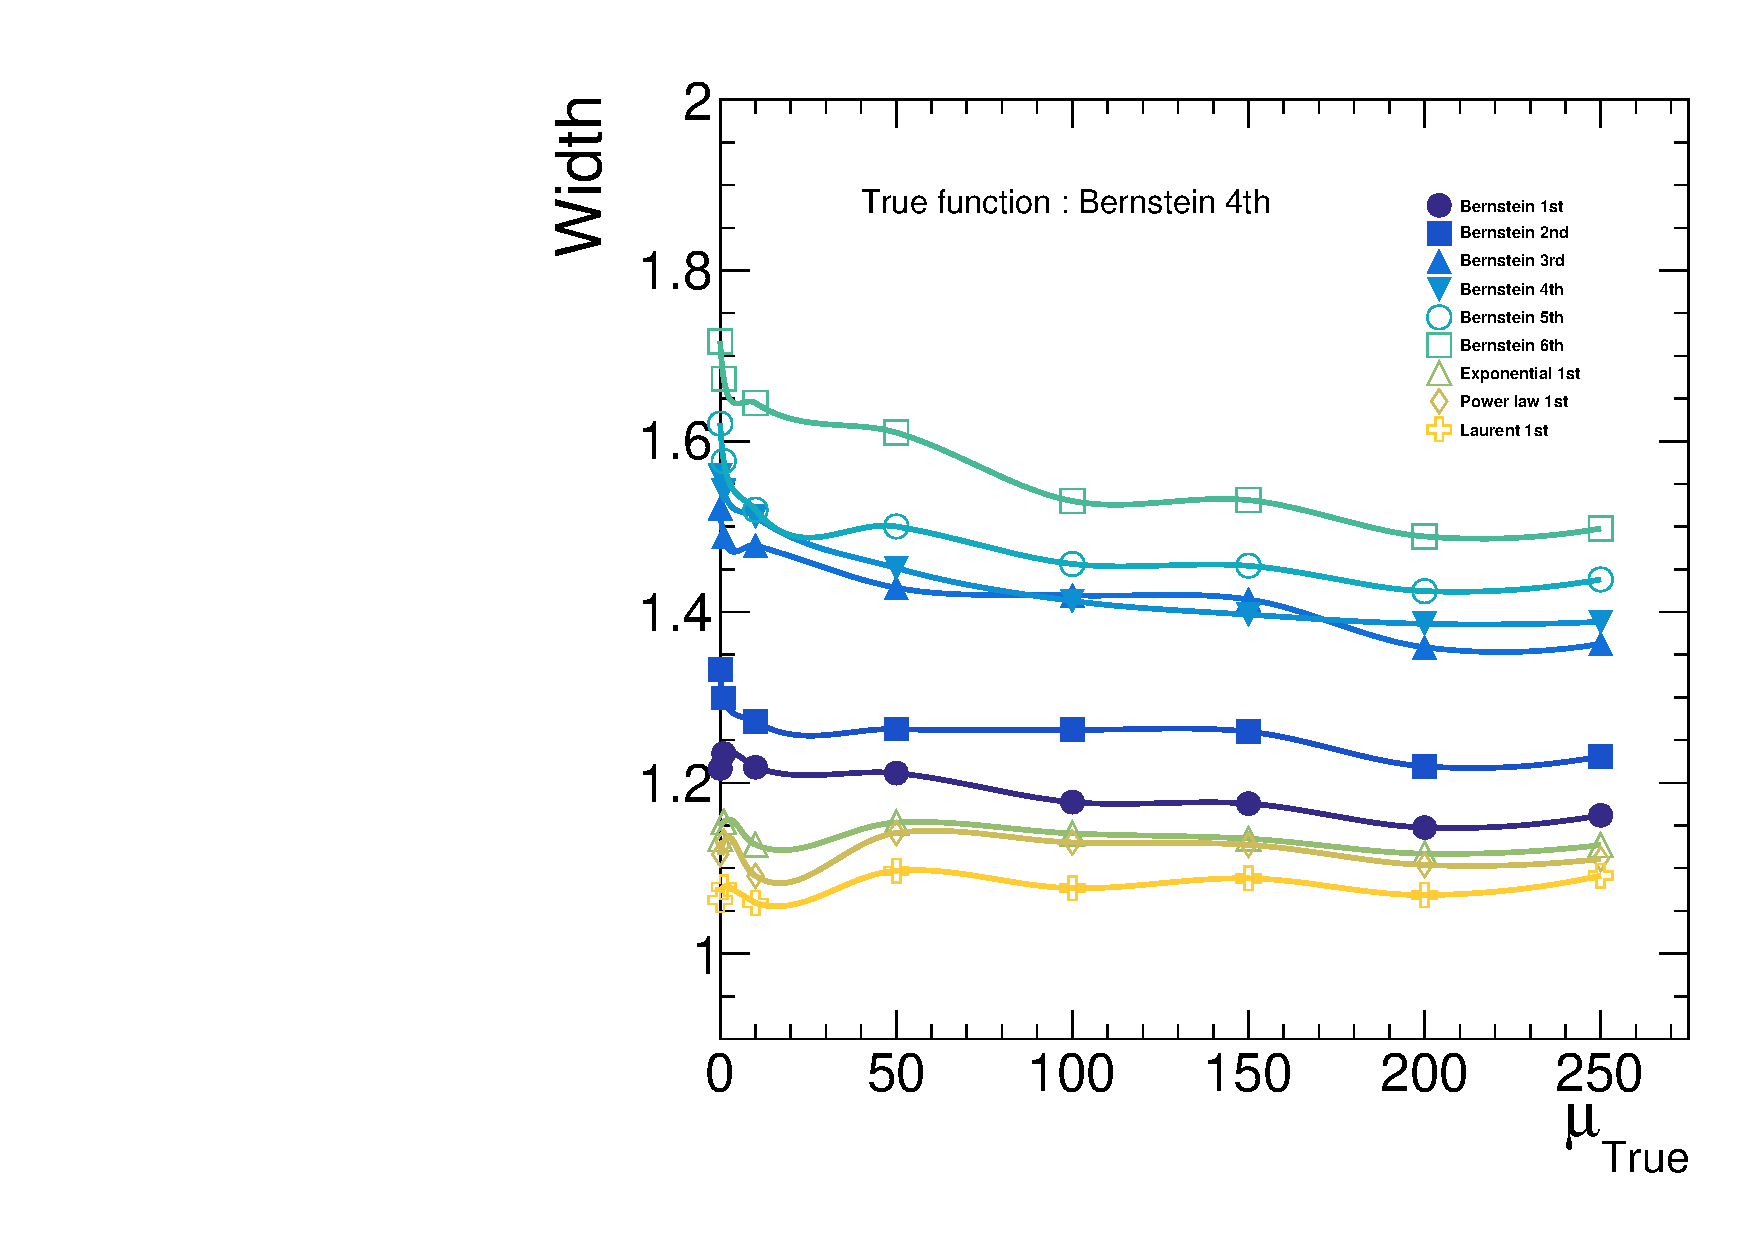
\includegraphics[width=0.33\textwidth]{Fig/BiasStudy/Linearity/ZJpsiG_Cat2/pull_width_linearity_TrueFunc3}~
  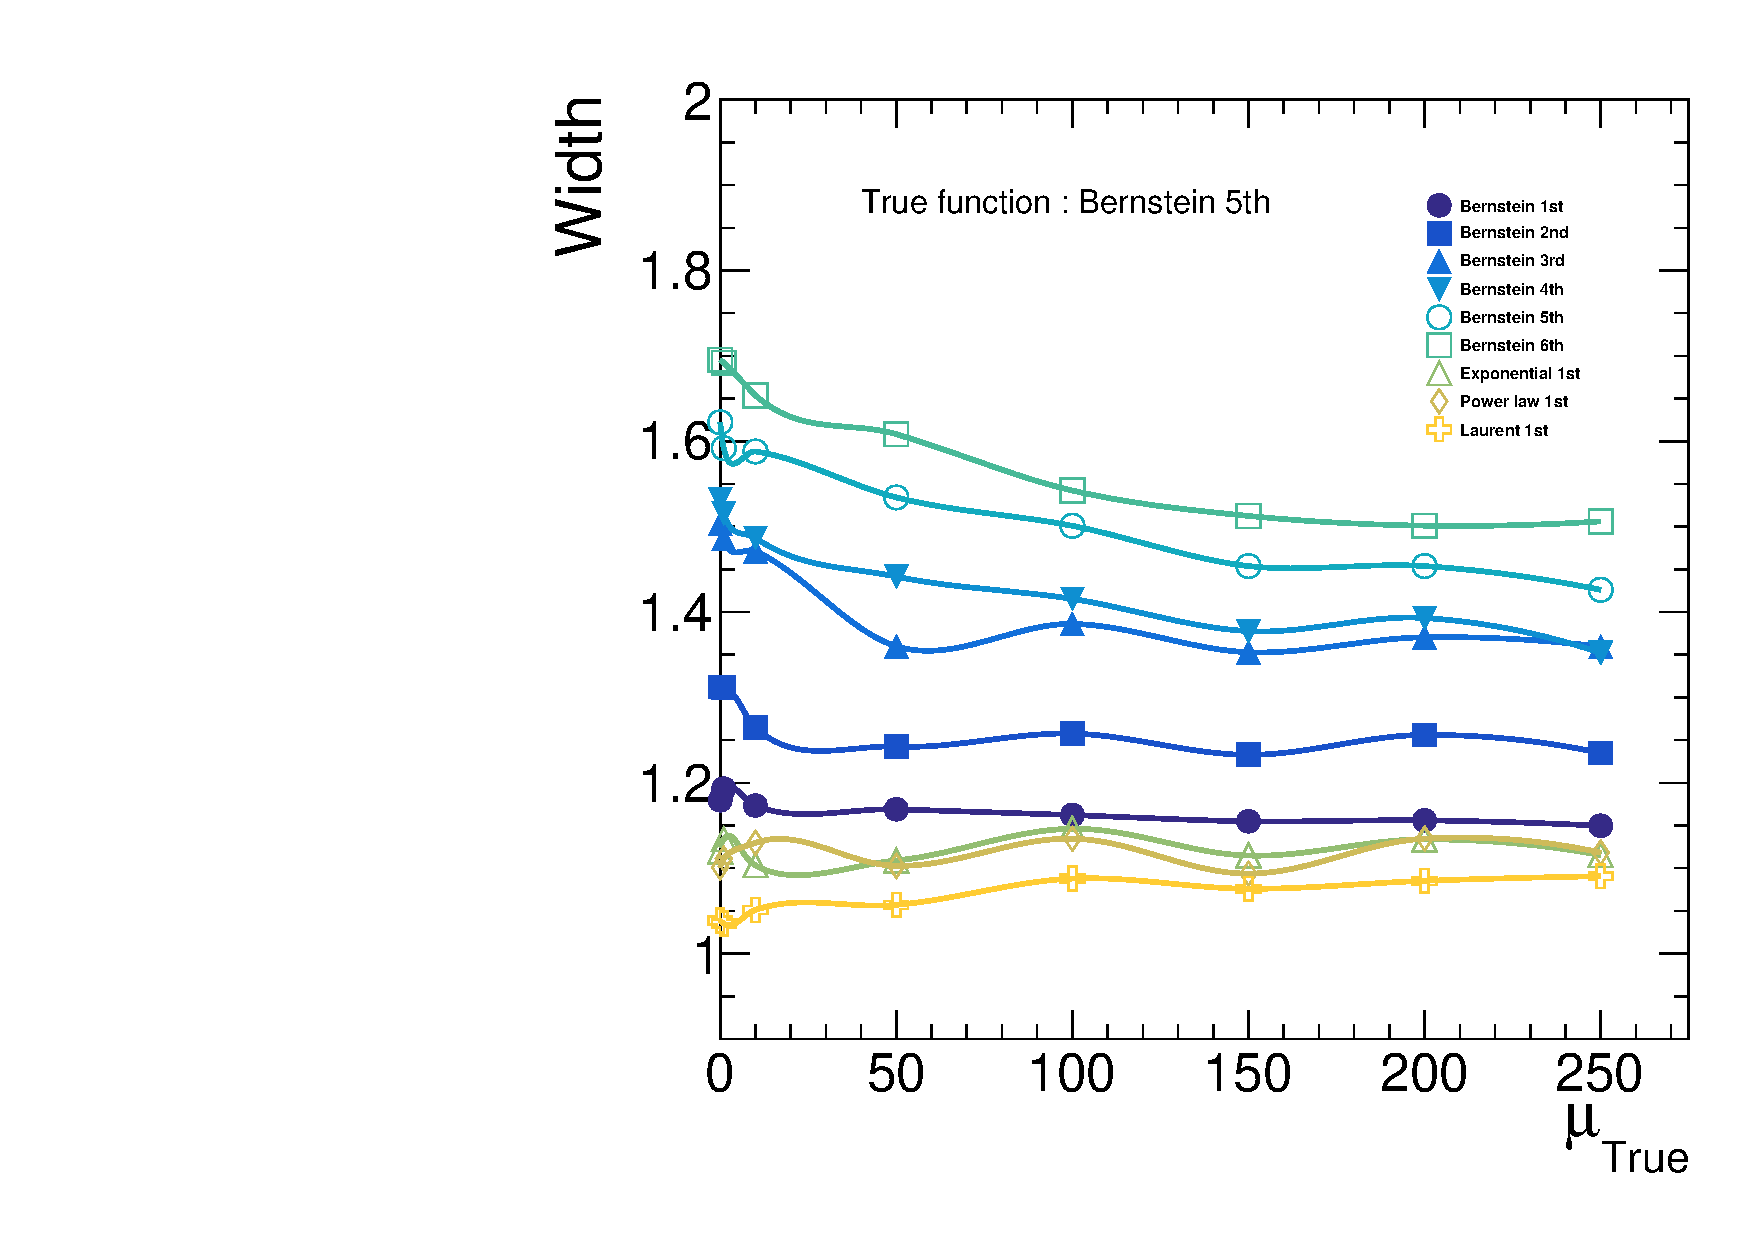
\includegraphics[width=0.33\textwidth]{Fig/BiasStudy/Linearity/ZJpsiG_Cat2/pull_width_linearity_TrueFunc4}~
  \includegraphics[width=0.33\textwidth]{Fig/BiasStudy/Linearity/ZJpsiG_Cat2/pull_width_linearity_TrueFunc5}\\
  \includegraphics[width=0.33\textwidth]{Fig/BiasStudy/Linearity/ZJpsiG_Cat2/pull_width_linearity_TrueFunc6}~
  \includegraphics[width=0.33\textwidth]{Fig/BiasStudy/Linearity/ZJpsiG_Cat2/pull_width_linearity_TrueFunc7}~
  \includegraphics[width=0.33\textwidth]{Fig/BiasStudy/Linearity/ZJpsiG_Cat2/pull_width_linearity_TrueFunc8}\\
  \caption{The evolution of the width of the pull value distribution as more signal events are introduced in the Cat2 of the Z decay.}
  \label{fig:Linearity_width_ZJpsiG_Cat2}
\end{figure}
\clearpage

\subsection{$Z\to \JPsi\ \gamma$ Cat3}
\begin{figure}[!ht]
  \centering
  \includegraphics[width=0.33\textwidth]{Fig/BiasStudy/Linearity/ZJpsiG_Cat3/pull_mean_linearity_TrueFunc0}~
  \includegraphics[width=0.33\textwidth]{Fig/BiasStudy/Linearity/ZJpsiG_Cat3/pull_mean_linearity_TrueFunc1}~
  \includegraphics[width=0.33\textwidth]{Fig/BiasStudy/Linearity/ZJpsiG_Cat3/pull_mean_linearity_TrueFunc2}\\
  \includegraphics[width=0.33\textwidth]{Fig/BiasStudy/Linearity/ZJpsiG_Cat3/pull_mean_linearity_TrueFunc3}~
  \includegraphics[width=0.33\textwidth]{Fig/BiasStudy/Linearity/ZJpsiG_Cat3/pull_mean_linearity_TrueFunc4}~
  \includegraphics[width=0.33\textwidth]{Fig/BiasStudy/Linearity/ZJpsiG_Cat3/pull_mean_linearity_TrueFunc5}\\
  \includegraphics[width=0.33\textwidth]{Fig/BiasStudy/Linearity/ZJpsiG_Cat3/pull_mean_linearity_TrueFunc6}~
  \includegraphics[width=0.33\textwidth]{Fig/BiasStudy/Linearity/ZJpsiG_Cat3/pull_mean_linearity_TrueFunc7}~
  \includegraphics[width=0.33\textwidth]{Fig/BiasStudy/Linearity/ZJpsiG_Cat3/pull_mean_linearity_TrueFunc8}\\
  \caption{The evolution of the mean of the pull value distribution as more signal events are introduced in the Cat3 of the Z decay.}
  \label{fig:Linearity_mean_ZJpsiG_Cat3}
\end{figure}
\clearpage
%
\begin{figure}[!ht]
  \centering
  \includegraphics[width=0.33\textwidth]{Fig/BiasStudy/Linearity/ZJpsiG_Cat3/pull_width_linearity_TrueFunc0}~
  \includegraphics[width=0.33\textwidth]{Fig/BiasStudy/Linearity/ZJpsiG_Cat3/pull_width_linearity_TrueFunc1}~
  \includegraphics[width=0.33\textwidth]{Fig/BiasStudy/Linearity/ZJpsiG_Cat3/pull_width_linearity_TrueFunc2}\\
  \includegraphics[width=0.33\textwidth]{Fig/BiasStudy/Linearity/ZJpsiG_Cat3/pull_width_linearity_TrueFunc3}~
  \includegraphics[width=0.33\textwidth]{Fig/BiasStudy/Linearity/ZJpsiG_Cat3/pull_width_linearity_TrueFunc4}~
  \includegraphics[width=0.33\textwidth]{Fig/BiasStudy/Linearity/ZJpsiG_Cat3/pull_width_linearity_TrueFunc5}\\
  \includegraphics[width=0.33\textwidth]{Fig/BiasStudy/Linearity/ZJpsiG_Cat3/pull_width_linearity_TrueFunc6}~
  \includegraphics[width=0.33\textwidth]{Fig/BiasStudy/Linearity/ZJpsiG_Cat3/pull_width_linearity_TrueFunc7}~
  \includegraphics[width=0.33\textwidth]{Fig/BiasStudy/Linearity/ZJpsiG_Cat3/pull_width_linearity_TrueFunc8}\\
  \caption{The evolution of the width of the pull value distribution as more signal events are introduced in the Cat3 of the Z decay.\label{fig:Linearity_width_ZJpsiG_Cat3}}
\end{figure}
\clearpage
%
\section{Pseudo-event}
Examples of pseudo-events for the Higgs and all the three categories of Z boson searches are shown in this section. 
The pseudo-events are generated from the least-bias functions for each category. The fits using the least-bias functions are also shown in the plots, where the green one is the signal component of the resulting fit, red one is the background component, and the blue one is the combination of the signal and background component.
\clearpage
\subsection{Pseudo-events for $H\to \JPsi\ \gamma$}
\begin{figure}[!ht]
  \centering
  \includegraphics[width=0.33\textwidth]{Fig/BiasStudy/Toys/HJpsiG/TruePdf1_FitPdf1_mu300_sbfit_1232_cat1}~
  \includegraphics[width=0.33\textwidth]{Fig/BiasStudy/Toys/HJpsiG/TruePdf1_FitPdf1_mu300_sbfit_12345_cat1}~
  \includegraphics[width=0.33\textwidth]{Fig/BiasStudy/Toys/HJpsiG/TruePdf1_FitPdf1_mu300_sbfit_12321_cat1}\\
  \includegraphics[width=0.33\textwidth]{Fig/BiasStudy/Toys/HJpsiG/TruePdf1_FitPdf1_mu300_sbfit_12318_cat1}~
  \includegraphics[width=0.33\textwidth]{Fig/BiasStudy/Toys/HJpsiG/TruePdf1_FitPdf1_mu300_sbfit_12337_cat1}~
  \includegraphics[width=0.33\textwidth]{Fig/BiasStudy/Toys/HJpsiG/TruePdf1_FitPdf1_mu300_sbfit_12333_cat1}\\
  \includegraphics[width=0.33\textwidth]{Fig/BiasStudy/Toys/HJpsiG/TruePdf1_FitPdf1_mu300_sbfit_1237_cat1}~
  \includegraphics[width=0.33\textwidth]{Fig/BiasStudy/Toys/HJpsiG/TruePdf1_FitPdf1_mu300_sbfit_12324_cat1}~
  \includegraphics[width=0.33\textwidth]{Fig/BiasStudy/Toys/HJpsiG/TruePdf1_FitPdf1_mu300_sbfit_12346_cat1}\\
  \caption{Examples of the pseudo-events for bias study in Higgs search. The toys are generated from Bernstein polynomial of 2nd order, and the background fit (red line) is the Bernstein polynomial of 2nd order.\label{fig:Toys_HJpsiG}}
\end{figure}
\clearpage

\subsection{Pseudo-events for Cat1 of $\cPZ\to\JPsi\ \gamma$}
\begin{figure}[!ht]
  \centering
  \includegraphics[width=0.33\textwidth]{Fig/BiasStudy/Toys/ZJpsiG_Cat1/TruePdf2_FitPdf2_mu200_sbfit_12350_cat1}~
  \includegraphics[width=0.33\textwidth]{Fig/BiasStudy/Toys/ZJpsiG_Cat1/TruePdf2_FitPdf2_mu200_sbfit_1231_cat1}~
  \includegraphics[width=0.33\textwidth]{Fig/BiasStudy/Toys/ZJpsiG_Cat1/TruePdf2_FitPdf2_mu200_sbfit_12345_cat1}\\
  \includegraphics[width=0.33\textwidth]{Fig/BiasStudy/Toys/ZJpsiG_Cat1/TruePdf2_FitPdf2_mu200_sbfit_12328_cat1}~
  \includegraphics[width=0.33\textwidth]{Fig/BiasStudy/Toys/ZJpsiG_Cat1/TruePdf2_FitPdf2_mu200_sbfit_12339_cat1}~
  \includegraphics[width=0.33\textwidth]{Fig/BiasStudy/Toys/ZJpsiG_Cat1/TruePdf2_FitPdf2_mu200_sbfit_12314_cat1}\\
  \includegraphics[width=0.33\textwidth]{Fig/BiasStudy/Toys/ZJpsiG_Cat1/TruePdf2_FitPdf2_mu200_sbfit_12319_cat1}~
  \includegraphics[width=0.33\textwidth]{Fig/BiasStudy/Toys/ZJpsiG_Cat1/TruePdf2_FitPdf2_mu200_sbfit_12321_cat1}~
  \includegraphics[width=0.33\textwidth]{Fig/BiasStudy/Toys/ZJpsiG_Cat1/TruePdf2_FitPdf2_mu200_sbfit_1237_cat1}\\
  \caption{Examples of the pseudo-events for bias study in Cat1 of Z search. The toys are generated from Bernstein polynomial of 3rd order, and the background fit (red line) is the Bernstein polynomial of 3rd order.}
  \label{fig:Toys_ZJpsiG_Cat1}
\end{figure}
\clearpage

\subsection{Pseudo-events for Cat2 of $Z\to \JPsi\ \gamma$}
\begin{figure}[!ht]
  \centering
  \includegraphics[width=0.33\textwidth]{Fig/BiasStudy/Toys/ZJpsiG_Cat2/TruePdf2_FitPdf2_mu200_sbfit_12324_cat2}~
  \includegraphics[width=0.33\textwidth]{Fig/BiasStudy/Toys/ZJpsiG_Cat2/TruePdf2_FitPdf2_mu200_sbfit_12315_cat2}~
  \includegraphics[width=0.33\textwidth]{Fig/BiasStudy/Toys/ZJpsiG_Cat2/TruePdf2_FitPdf2_mu200_sbfit_1234_cat2}\\
  \includegraphics[width=0.33\textwidth]{Fig/BiasStudy/Toys/ZJpsiG_Cat2/TruePdf2_FitPdf2_mu200_sbfit_12331_cat2}~
  \includegraphics[width=0.33\textwidth]{Fig/BiasStudy/Toys/ZJpsiG_Cat2/TruePdf2_FitPdf2_mu200_sbfit_12313_cat2}~
  \includegraphics[width=0.33\textwidth]{Fig/BiasStudy/Toys/ZJpsiG_Cat2/TruePdf2_FitPdf2_mu200_sbfit_1239_cat2}\\
  \includegraphics[width=0.33\textwidth]{Fig/BiasStudy/Toys/ZJpsiG_Cat2/TruePdf2_FitPdf2_mu200_sbfit_12344_cat2}~
  \includegraphics[width=0.33\textwidth]{Fig/BiasStudy/Toys/ZJpsiG_Cat2/TruePdf2_FitPdf2_mu200_sbfit_12336_cat2}~
  \includegraphics[width=0.33\textwidth]{Fig/BiasStudy/Toys/ZJpsiG_Cat2/TruePdf2_FitPdf2_mu200_sbfit_12310_cat2}\\
  \caption{Examples of the pseudo-events for bias study in Cat2 of Z search. The toys are generated from Bernstein polynomial of 3rd order, and the background fit (red line) is the Bernstein polynomial of 3rd order.}
  \label{fig:Toys_ZJpsiG_Cat2}
\end{figure}
\clearpage

\subsection{Pseudo-events for Cat3 of $Z\to \JPsi\ \gamma$}
\begin{figure}[!ht]
  \centering
  \includegraphics[width=0.33\textwidth]{Fig/BiasStudy/Toys/ZJpsiG_Cat3/TruePdf2_FitPdf2_mu200_sbfit_1231_cat3}~
  \includegraphics[width=0.33\textwidth]{Fig/BiasStudy/Toys/ZJpsiG_Cat3/TruePdf2_FitPdf2_mu200_sbfit_1235_cat3}~
  \includegraphics[width=0.33\textwidth]{Fig/BiasStudy/Toys/ZJpsiG_Cat3/TruePdf2_FitPdf2_mu200_sbfit_12349_cat3}\\
  \includegraphics[width=0.33\textwidth]{Fig/BiasStudy/Toys/ZJpsiG_Cat3/TruePdf2_FitPdf2_mu200_sbfit_12336_cat3}~
  \includegraphics[width=0.33\textwidth]{Fig/BiasStudy/Toys/ZJpsiG_Cat3/TruePdf2_FitPdf2_mu200_sbfit_12324_cat3}~
  \includegraphics[width=0.33\textwidth]{Fig/BiasStudy/Toys/ZJpsiG_Cat3/TruePdf2_FitPdf2_mu200_sbfit_12327_cat3}\\
  \includegraphics[width=0.33\textwidth]{Fig/BiasStudy/Toys/ZJpsiG_Cat3/TruePdf2_FitPdf2_mu200_sbfit_12315_cat3}~
  \includegraphics[width=0.33\textwidth]{Fig/BiasStudy/Toys/ZJpsiG_Cat3/TruePdf2_FitPdf2_mu200_sbfit_12316_cat3}~
  \includegraphics[width=0.33\textwidth]{Fig/BiasStudy/Toys/ZJpsiG_Cat3/TruePdf2_FitPdf2_mu200_sbfit_12318_cat3}\\
  \caption{Examples of the pseudo-events for bias study in Cat3 of Z search. The toys are generated from Bernstein polynomial of 3rd order, and the background fit (red line) is the Bernstein polynomial of 3rd order.}
  \label{fig:Toys_ZJpsiG_Cat3}
\end{figure}
\clearpage